\documentclass[conference]{IEEEtran}
\IEEEoverridecommandlockouts

% Core packages
\usepackage{cite}
\usepackage[T1]{fontenc}
\usepackage{hyperref}

% Math packages
\usepackage{amsmath,amssymb,amsfonts}
\usepackage{array,booktabs}

% Graphics and layout
\usepackage{graphicx}
\usepackage{subcaption}
\usepackage{float}
\usepackage{multirow}
\usepackage{multicol}
\usepackage{balance}

% Algorithm and code
\usepackage{algorithm}
\usepackage{algpseudocode} 
\usepackage{algorithmicx}
\usepackage{listings}

% Text and formatting
\usepackage{textcomp}
\usepackage{url}
\usepackage{enumitem}
\usepackage{caption} 
\usepackage{tcolorbox}
\usepackage{empheq}
\usepackage{varwidth}
\usepackage{balance}
\usepackage{todonotes}
\usepackage{flushend} 
\usepackage{stfloats}

\usepackage[ngerman,main=english]{babel}
 
% TikZ for diagrams
\usepackage{tikz}
\usetikzlibrary{arrows.meta,shapes,positioning}
\usetikzlibrary{calc,angles,quotes}

% --- Macro for drawing a 2D spherocylinder ---
% #1 = center coordinate
% #2 = rotation angle
% #3 = half-length
% #4 = radius
\newcommand{\drawSpherocyl}[4]{
    \begin{scope}[shift={(#1)},rotate=#2]
        \draw[line width=1pt,rounded corners=6pt] (-#3 + #4,#4) -- (#3 - #4,#4);
        \draw[line width=1pt,rounded corners=6pt] (-#3 + #4,-#4) -- (#3 - #4,-#4);
        \draw[line width=1pt,rounded corners=6pt] (#3 - #4,-#4) arc[start angle=-90,end angle=90,radius=#4];
        \draw[line width=1pt,rounded corners=6pt] (-#3 + #4,#4) arc[start angle=90,end angle=270,radius=#4];
        \fill [black] (#1) circle (2pt);
    \end{scope}
}



\hypersetup{hidelinks}
\DeclareMathAlphabet\mathbfcal{OMS}{cmsy}{b}{n}

% Macro for growth comparison row
\newcolumntype{M}[1]{>{\centering\arraybackslash}m{#1}}

\newcommand{\growthcomparisonrow}[6]{%
    #1 &
        \includegraphics[width=\linewidth]{figures/growth/#1_#2/#1_#2.#3.jpeg}
    &
        \includegraphics[width=\linewidth]{figures/growth/#1_#2/#1_#2.#4.jpeg}
    &
        \includegraphics[width=\linewidth]{figures/growth/#1_#2/#1_#2.#5.jpeg}
    &
        \includegraphics[width=\linewidth]{figures/growth/#1_#2/#1_#2.#6.jpeg}
    \\
}

\newcommand{\orientationcomparisonrow}[2]{%
    #1 &
        \includegraphics[width=\linewidth]{figures/orientation_comparisons/zoomed_images/hard_e#2_orient.jpeg}
    &   
        \includegraphics[width=\linewidth]{figures/orientation_comparisons/zoomed_images/soft_e#2_orient.jpeg}
    \\
}
 
\newcommand{\algorithmautorefname}{Algorithm}


\begin{document}

\title{Proliferating Cell Collectives: \\A Comparison of Hard and Soft Collision Models}

\author{
    \IEEEauthorblockN{Manuel Lerchner}
    \IEEEauthorblockA{
        \textit{Technical University of Munich}\\
        Munich, Germany}
}

\maketitle

\begin{abstract}
    This work extends the hard (constraint-based) collision model introduced by Weady et al.~\cite{Weady2024} by systematically comparing it with a soft (potential-based) approach for simulating proliferating cell collectives. Both models are implemented within a unified computational framework, enabling direct benchmarking of bacterial colony growth.

    Our results show that both approaches reproduce key experimentally observed patterns, including concentric rings and microdomain formation, but they involve distinct trade-offs. The hard model permits timesteps roughly 30 times larger than the soft model, though at a higher per-step cost due to solving a global constraint system. In contrast, the soft model suffers from numerical stiffness and allows unphysical cell overlap, producing packing fractions exceeding 5 in colony centers compared to the hard model's realistic 0.9.

    We also introduce an adaptive timestepping algorithm based on the Courant-Friedrichs-Lewy condition to dynamically select stable timesteps. Benchmarking reveals the hard model excels for small to moderate colonies ($R \leq 100$), while the soft model's scalability enables faster simulations for larger systems.

    Despite microscopic differences in packing and stress, both models produce similar macroscopic patterns, indicating that colony-level behavior is largely robust to the collision resolution method. We find that the soft model offers an efficient and biologically plausible option for large-scale studies, whereas the hard model is preferable when precise stress calculations or geometric fidelity are required.
\end{abstract}

\begin{IEEEkeywords}
    collision models, constraint-based simulation, potential-based repulsion, bacterial colony growth, proliferating cell collectives, adaptive timestepping, pattern formation, computational performance, stress-sensitive growth, microdomain formation
\end{IEEEkeywords}

\section{Introduction}
\subsection{Biological Motivation}

The collective behaviors of biological entities, from microbial colonies to multicellular tissues, exemplify how local interactions among individual organisms can generate complex, large-scale structures and dynamics. These systems often exhibit emergent spatio-temporal patterns that arise from the interplay of cell growth, division, mechanical interactions, and local environmental feedback. Understanding such patterns is essential for comprehending fundamental biological processes and has applications ranging from biofilm formation to tissue engineering.

A particularly compelling example is found in bacterial colonies, where cell arrangement reflects growth dynamics and internal stresses. Continuous cell proliferation within colonies generates significant mechanical forces that accumulate in the densely packed interior~\cite{Wittmann2023}, leading to compressive stresses that suppress cell growth at the colony center. As a result, peripheral cells expand outward over time while internal cells remain densely packed and growth-limited. This outward expansion over time produces the characteristic concentric ring patterns observed in bacterial species such as \textit{E. coli}, \textit{Bacillus subtilis}, and \textit{Proteus mirabilis}, as well as fungi like \textit{Setosphaeria rostrata} and \textit{Exserohilum turcicum}, as illustrated in \autoref{fig:exserohilum_turcicum}~\cite{YAMAZAKI2005136}.

\begin{figure}[t]
    \centering
    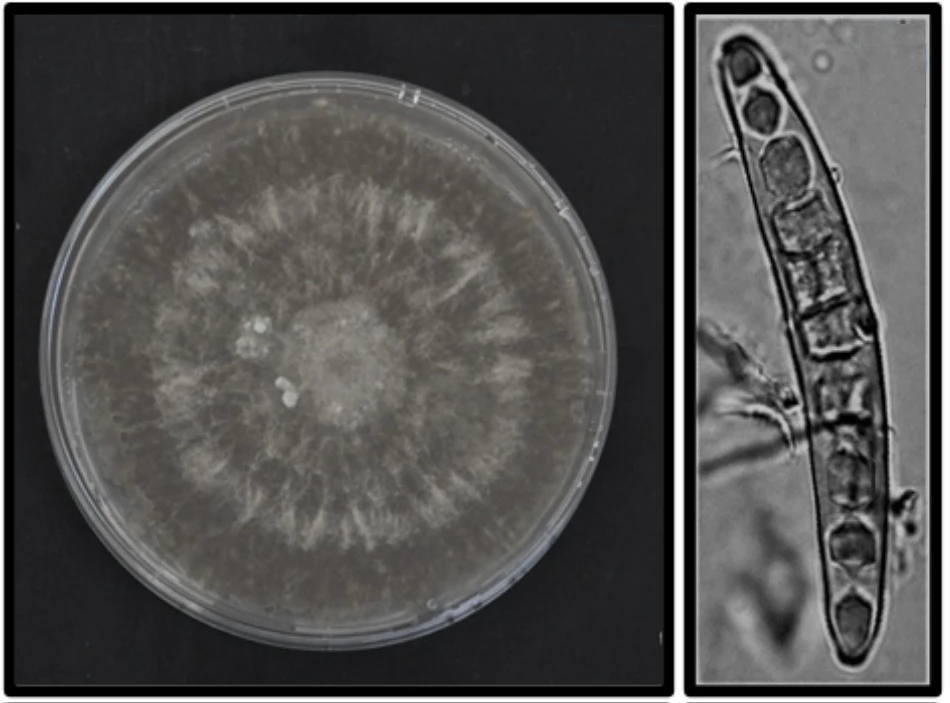
\includegraphics[width=\linewidth]{figures/real-bacteria/Exserohilum turcicum.png}
    \caption{Morphology of the fungus \textit{Exserohilum turcicum}. The left image shows a typical colony with concentric ring patterns, while the right image displays the elongated, rod-shaped morphology of individual fungal cells. Source:~\cite{Bankole2023}.}
    \label{fig:exserohilum_turcicum}
\end{figure}

Computational modeling offers a powerful tool for dissecting the complex dynamics and emergent spatial patterns observed in those colonies. To reproduce such emergent structures and uncover their underlying mechanisms, models must accurately capture the dynamic interplay between cell growth and division, mechanical forces, and intercellular interactions.

Simulating dense, proliferating cell collectives, however, poses significant computational challenges: the large number of cells in realistic colonies, combined with the need to resolve collisions accurately across continuously changing configurations, creates a computational bottleneck. Moreover, different collision-handling approaches, such as rigid constraints versus soft repulsions, offer distinct trade-offs in physical fidelity, numerical stability, and computational cost. This work is directly motivated by these considerations and builds upon the pioneering computational framework developed by Weady et al.~\cite{Weady2024}, who demonstrated how to model bacterial colony growth while capturing stress-dependent feedback and pattern formation. We extend their work by systematically comparing two fundamentally different approaches to collision handling, examining their respective strengths and limitations in simulating large systems of proliferating cells.



\section{Related Work}

\subsection{Collision Modeling Paradigms}

In computational biology, agent-based models (ABMs) represent individual cells as discrete entities that grow, divide, and interact mechanically. Unlike continuum models, which treat populations as continuous fields, ABMs simulate single-cell behavior and local heterogeneity. A central computational challenge in such models is resolving cell-cell collisions efficiently. Two primary paradigms exist for handling collisions: soft (potential-based) collision models and hard (constraint-based) collision models.

\begin{description}[style=nextline]
    \item[Soft (Potential-Based) Models]
        Soft models manage cell interactions through repulsive forces defined by potentials such as Hertzian or Lennard-Jones functions. When cells overlap, these forces push them apart continuously. The primary advantage is computational efficiency: the calculations are local and embarrassingly parallelizable, enabling large-scale simulations. For instance, Warren et al.~\cite{Warren2019} demonstrated this by simulating millions of cells in three dimensions using a soft repulsion approach.

        However, soft models suffer from two key limitations. First, the stiffness of repulsive potentials creates numerical instability, requiring very small timesteps to maintain accuracy and prevent divergence. Second, the finite range of repulsive forces means cells behave as elastically deformable objects rather than rigid bodies, effectively reducing their geometric diameter below the intended size~\cite{Yan2019}. This deformation accumulates and can distort simulation results, particularly in dense regions.

    \item[Hard (Constraint-Based) Models]
        Hard models enforce strict non-overlapping constraints, treating cells as geometrically rigid and impenetrable. Constraint-based methods are widely used in physics simulations~\cite{Tasora2008,Macklin2014,Li2021,Ferguson2021}, and have also been adapted for biological systems~\cite{Rudge2012,Weady2024,Yan2019}.

        The main drawback is computational cost and added complexity. Enforcing global non-overlap constraints requires iterative solvers operating on large coupled systems of equations, which creates a significant bottleneck. Modern implementations, however, can efficiently reduce the numerical stiffness associated with soft models, enabling much larger timesteps while maintaining geometric fidelity~\cite{Yan2019}. Nonetheless, the fundamental trade-off remains: higher cost per timestep due to constraint solving, but fewer timesteps required overall.
\end{description}

\subsection{The Benchmarking Gap}

While soft and hard collision models entail distinct computational trade-offs, the question of which approach offers better performance remains unresolved. This trade-off becomes particularly critical when simulating large populations of independent agents, where the choice of collision model directly affects runtime, scalability, and the accuracy of the simulation.

To our knowledge, a direct, systematic comparison of these models is absent from the literature. Moreover, existing biological studies typically validate their chosen approach against experimental data, such as microscopy images, growth curves, and morphological features~\cite{Rudge2012,Weady2024,Blanchard2015,Ghosh2015,You2018,Warren2019,Khan_2024,You_2021,Valdez2025,Rudge2013,Langeslay_2023}, prioritizing biological accuracy over computational performance. Few studies provide rigorous benchmarking of runtime, scalability, or numerical stability across different colony sizes. Consequently, modelers lack clear guidance on which paradigm is more efficient for a given problem scale.

This work aims to address this gap by implementing both soft and hard collision schemes within a shared computational framework, enabling direct performance comparisons. We systematically benchmark the two approaches across a range of colony sizes, evaluating their respective strengths and limitations in both biological fidelity and computational efficiency.

\section{Cell Mechanics}

Accurately modeling mechanical interactions between cells is essential for simulating colony growth and emergent spatial patterns. From a computational perspective, approximating bacteria and fungi as rigid spherocylinders (rods with hemispherical end caps) offers a balance between biological realism and computational efficiency. This representation captures the elongated morphology of these organisms while preserving the fundamental mechanics of cell-cell interactions and colony expansion. Although real cells exhibit some deformability, the rigid spherocylinder approximation successfully captures essential collective dynamics at significantly reduced computational cost and is well validated experimentally~\cite{Rudge2012,Khan_2024,Rudge2013,Langeslay_2023,Ghosh2015}. The spherocylinder geometry closely matches common organisms such as \textit{E. coli} and \textit{Setosphaeria rostrata} (see \autoref{fig:exserohilum_turcicum}), and has become standard in computational models of microbial collectives~\cite{You2018, Weady2024, Blanchard2015, Warren2019, Ghosh2015}.

Each spherocylinder is characterized by a time-varying length $\ell$ that increases during growth prior to division, and a fixed diameter $d$ that remains constant across the population. This geometry enables efficient contact detection algorithms~\cite{GeometricTools} and naturally accommodates rotational dynamics essential for capturing realistic colony mechanics.

At bacterial length scales, the Reynolds number is extremely small ($\text{Re} \ll 1$), so viscous forces dominate over inertia. In this highly viscous, \textit{sticky} environment, cells stop almost immediately once forces cease~\cite{datta2024lifelowreynoldsnumber,Rudge2012}. As a result, cell motion is governed by the overdamped Langevin equation:

\begin{equation} \label{eq:overdamped_langevin}
    \mathbf{u}_i = \frac{1}{\zeta \ell_i} \sum_{j \neq i} \mathbf{F}_{ij}, \quad
    \boldsymbol{\omega}_i = \frac{12}{\zeta \ell_i^3} \sum_{j \neq i} \mathbf{r}_{ij} \times \mathbf{F}_{ij}
\end{equation}

Here, $\mathbf{u}_i$ and $\boldsymbol{\omega}_i$ are the translational and angular velocities of cell $i$, $\mathbf{F}_{ij}$ is the force exerted on cell $i$ by cell $j$, $\zeta$ is the drag coefficient, and $\mathbf{r}_{ij}$ is the lever arm from the cell center to the contact point. \autoref{fig:spherocylinder_model} illustrates the model and the forces and torques during collision.
\subsection{Cell Growth and Division}

Bacterial cells grow along their longitudinal axis according to the following model, adapted from~\cite{Weady2024SM}:

\begin{equation} \label{eq:growth}
    \dot{\ell}_i = \frac{\ell_i}{\tau} e^{-\lambda \sigma_i}
\end{equation}

where $\tau$ is a characteristic timescale, $\sigma_i$ is the compressive stress along cell $i$'s main axis, and $\lambda$ is a stress sensitivity parameter. As the compressive stress increases, the effective growth rate $\dot{\ell}_i$ decreases toward zero, leading to slower elongation. When $\sigma_i = 0$, the cell grows exponentially with a rate determined solely by $\tau$.

The stress on cell $i$ is computed by projecting contact forces onto the cell's longitudinal axis $\hat{\mathbf{t}}_i$:

\begin{equation} \label{eq:stress}
    \sigma_i = \sum_{j \neq i} \frac{1}{2} \left| \hat{\mathbf{t}}_i \cdot \mathbf{F}_{ij} \right|
\end{equation}

In our simulations, the initial cell is initialized with length $\ell = 1$ and diameter $d = 0.5$. Cell division occurs when a cell reaches a critical length $\ell_{\text{crit}} = 2$, producing two daughter cells with lengths randomly sampled from $\left[0.98\,\frac{\ell_{\text{crit}}}{2},\, 1.02\,\frac{\ell_{\text{crit}}}{2}\right]$ to prevent artificial synchronization of division events~\cite{You2018}.

\subsection{Rotational Diffusion}

To account for Brownian motion and other sources of random fluctuations, we apply a small rotational perturbation to each cell at every timestep. This introduces gradual rotational diffusion, preventing cells from forming artificially aligned configurations and promoting realistic spatial arrangements.

\begin{figure}[H]
    \centering

    \begin{tikzpicture}[line cap=round,line join=round,>=Stealth]

        % --- Variables ---
        \coordinate (xi) at (0.8,-0.5);
        \coordinate (xj) at (1.4,-1.8);

        \coordinate (x) at (-3,-0.5);
        \def\R{0.5}

        \drawSpherocyl{xi}{-10}{1.4}{\R}
        \drawSpherocyl{xj}{15}{1.3}{\R}

        \coordinate (contact) at  (1.85,-1.15);

        % Collision point
        \fill[black] (contact) circle (2pt) node[above right] {};

        % Force vector
        \draw[->,thick,red] (contact) -- ++($0.9*(-0.258,0.965)$) node[pos=0.9,left] {$\mathbf{F}_{ij}$};

        % Torque lever arm
        \draw[->,thick,blue,dashed] (xi) -- (contact) node[pos=0.2,below] {$\mathbf{r}_{ij}$};

        % Force vector
        \draw[->,thick,red] (contact) -- ++($0.8*(0.258,-0.965)$) node[pos=0.6,right] {$\mathbf{F}_{ji}$};

        % Torque lever arm
        \draw[->,thick,blue,dashed] (xj) -- (contact) node[pos=0.3,left] {$\mathbf{r}_{ji}$};



        % label at xi
        \node at (xi) [left] {$\mathbf{x}_i$};
        % label at xj
        \node at (xj) [below] {$\mathbf{x}_j$};


        \drawSpherocyl{x}{0}{2}{\R};

        % Add division constriction: two daughters forming
        \coordinate (left_daughter) at ($(x)+(-1,-1.25)$);
        \coordinate (right_daughter) at ($(x)+(1, -1.25)$);

        \drawSpherocyl{left_daughter}{0}{1}{\R};
        \drawSpherocyl{right_daughter}{0}{1}{\R};


        % label at x
        \node at (x) [below] {$\mathbf{x}$};
        % label at left daughter
        \node at (left_daughter) [below] {$\mathbf{x}_\text{left}$};
        % label at right daughter
        \node at (right_daughter) [below] {$\mathbf{x}_\text{right}$};

        \draw[<->,thick,dashed] ($(x) + (-2,0.8)$) -- ($(x) + (2,0.8)$) node[midway,above] {$\ell_{\text{crit}}$};

        \draw[<->,thick,dashed] ($(x) + (-1.3-\R-\R,-\R)$) -- ($(x) + (-1.3-\R-\R,\R)$) node[midway,left] {$d$};

        \draw[<->,thick,dashed] ($(right_daughter) + (-2.3-\R-\R,-\R)$) -- ($(right_daughter) + (-2.3-\R-\R,\R)$) node[midway,left] {$d$};

        \draw[<->,thick,dashed] ($(left_daughter) + (-1,-0.8)$) -- ($(left_daughter) + (1,-0.8)$) node[midway,below] {$\frac{\ell_{\text{crit}}}{2}$};

        \draw[<->,thick,dashed] ($(right_daughter) + (-1,-0.8)$) -- ($(right_daughter) + (1,-0.8)$) node[midway,below] {$\frac{\ell_{\text{crit}}}{2}$};



        % Resulting rotation around xi
        \draw[->,thick,orange]
        ($(xi)+(0.6,0.5)$) arc[start angle=0,end angle=160,radius=0.6]
        node[midway, below] {$\boldsymbol{\omega}_i$};


        % Resulting rotation around xj
        \draw[->,thick,orange]
        ($(xj)+(0.7,-0.5)$) arc[start angle=0,end angle=-150,radius=0.6]
        node[midway, above] {$\boldsymbol{\omega}_j$};

    \end{tikzpicture}
    \caption{Spherocylinder cell model. Contact forces $\mathbf{F}_{ij}$ (red) and lever arms $\mathbf{r}_{ij}$ (dashed blue) generate torques causing angular motion $\boldsymbol{\omega}$ (orange), and also produce translational displacements of the cells. Cell division occurs when a cell reaches critical length $\ell_{\text{crit}} = 2$.}
    \label{fig:spherocylinder_model}

\end{figure}

\newpage

\section{Unified Computational Framework}

\subsection{Colony Representation}

Following Weady et al.~\cite{Weady2024SM}, the bacterial colony is represented by a global state vector $\mathbfcal{C} = [\dots, \mathbf{x}_n^\top, \mathbf{q}_n^\top, \dots]^\top \in \mathbb{R}^{7N}$, where $N$ is the number of cells. Each cell is represented by a 7-dimensional sub-vector consisting of a position vector $\mathbf{x}_n \in \mathbb{R}^3$ and a unit quaternion $\mathbf{q}_n \in \mathbb{R}^4$ representing its orientation. The lengths of all cells are stored separately in a vector $\boldsymbol{\ell} = [\dots, \ell_n, \dots]^\top \in \mathbb{R}^{N}$. Quaternions are used instead of Euler angles or rotation matrices because they avoid singularities and provide stable numerical integration over long simulations.

\subsection{Colony Dynamics}

The translational and angular velocities of all cells in the colony from \autoref{eq:overdamped_langevin} are determined simultaneously by a force-velocity relationship $\mathbfcal{U} = \mathbfcal{M}^k \mathbfcal{F}$. Here, $\mathbfcal{F} \in \mathbb{R}^{6N}$ is the generalized force vector for the entire colony, containing both force and torque components for each cell. Similarly, $\mathbfcal{U} \in \mathbb{R}^{6N}$ is the generalized velocity vector containing the resulting translational and angular velocities. The vectors are defined as:

\begin{equation}
    \begin{alignedat}{5}
        \mathbfcal{F} &= [&\mathbf{f}_1,&\;\boldsymbol{\tau}_1,&\;\dots,&\;\mathbf{f}_N,&\;\boldsymbol{\tau}_N&]^\top \in \mathbb{R}^{6N}, \\
        \mathbfcal{U} &= [&\mathbf{u}_1,&\;\boldsymbol{\omega}_1,&\;\dots,&\;\mathbf{u}_N,&\;\boldsymbol{\omega}_N&]^\top \in \mathbb{R}^{6N}
    \end{alignedat}
\end{equation}

where, $\mathbf{f}_i = \sum_j \mathbf{F}_{ij}$ is the total force on cell $i$ due to all other cells $j$ in contact with it, and $\boldsymbol{\tau}_i = \sum_j \mathbf{r}_{ij} \times \mathbf{F}_{ij}$ is the total torque. The diagonal mobility matrix $\mathbfcal{M}^k$ at timestep $k$ encodes the drag coefficients for all cells based on their current lengths $\ell_i^k$:

\begin{equation}
    \mathbfcal{M}^k = \text{diag}\left(\frac{1}{\zeta \ell_1^k}\mathbf{I}_3, \frac{12}{\zeta {\ell_1^k}^3}\mathbf{I}_3, \dots \right) \in \mathbb{R}^{6N \times 6N}
\end{equation}

where $\mathbf{I}_3$ is the $3 \times 3$ identity matrix. The resulting matrix-vector product thus implements the overdamped Langevin equation from \autoref{eq:overdamped_langevin} for all cells simultaneously.

\subsection{State Integration}

The orientation quaternion $\mathbf{q}_n^k$ for each cell evolves according to the kinematic equation $\dot{\mathbf{q}}_n^k = \frac{1}{2} \boldsymbol{\omega}_n \otimes \mathbf{q}_n^k$, where $\otimes$ denotes quaternion multiplication. To integrate translational and rotational dynamics consistently, we introduce a mapping $\mathbfcal{G}^k \in \mathbb{R}^{7N \times 6N}$, converting Cartesian translational and angular velocities from $\mathbb{R}^{6N}$ into corresponding changes in positions and quaternions in $\mathbb{R}^{7N}$ according to the quaternion kinematics (see~\cite{Weady2024SM,Yan2022,Tasora2008}). Using $\mathbfcal{G}^k$, the colony's state and the length vector are updated via explicit Euler integration.

\begin{equation} \label{eq:colony_update}
    \begin{aligned}
        \mathbfcal{C}^{k+1}     & = \mathbfcal{C}^k + \Delta t \, \mathbfcal{G}^k \mathbfcal{U} = \mathbfcal{C}^k + \Delta t \, \mathbfcal{G}^k \mathbfcal{M}^k \mathbfcal{F} \\
        \boldsymbol{\ell}^{k+1} & = \boldsymbol{\ell}^k + \Delta t \, \dot{\boldsymbol{\ell}}
    \end{aligned}
\end{equation}

The distinction between hard and soft collision models lies solely in how the generalized force vector $\mathbfcal{F}$ and in particular the inter-cell forces $\mathbf{F}_{ij}$ are computed. The rest of the framework, including state representation, dynamics, and integration, remains identical.

\subsection{Soft Collision Model}

The soft collision model treats cell-cell interactions through continuous, potential-based repulsive forces. When cells overlap, these forces smoothly increase, preventing significant interpenetration while allowing elastic deformation. This approach is well-suited for simulating the soft, deformable nature of real biological cells and has been widely used in prior work~\cite{Warren2019, You2018,Blanchard2015,Ghosh2015,Khan_2024,You_2021,Valdez2025,Rudge2013,Langeslay_2023}.

We implement a Hertzian contact model, which describes elastic deformation between curved surfaces in contact. The repulsive elastic force exerted on cell $i$ by cell $j$ is:

\begin{equation} \label{eq:hertzian_contact_model}
    \mathbf{F}^{\text{elastic}}_{ij} = k_{cc} \sqrt{d} \, \delta^{3/2} \, \hat{\mathbf{n}}
\end{equation}

where $\delta$ is the overlap distance, $d$ is the cell diameter, $k_{cc}$ is an elastic constant, and $\hat{\mathbf{n}}$ is the unit normal vector at the contact point. The $\delta^{3/2}$ dependence is characteristic of Hertzian theory for elastic contacts and produces a nonlinear, smooth increase in force as overlap grows (see \autoref{fig:hertzian_contact_model}).

\subsubsection{Force Assembly}

The total force and torque on cell $n$ are computed by summing contributions from all pairwise elastic interactions and can be used to assemble the global force vector $\mathbfcal{F}$ and compute the cell growth rates $\dot{\boldsymbol{\ell}}$ via \autoref{eq:growth}:

\begin{equation} \label{eq:force_assembly}
    \mathbf{f}_i         = \sum_{j \neq i} \mathbf{F}^{\text{elastic}}_{ij}, \qquad
    \boldsymbol{\tau}_i  = \sum_{j \neq i} \mathbf{r}_{ij} \times \mathbf{F}^{\text{elastic}}_{ij}
\end{equation}

\subsubsection{Model Parameters and Numerical Stability}

The elastic constant is defined as $k_{cc} = \frac{Y}{\zeta}$, where $Y$ is the cell's Young's modulus and $\zeta$ is the fluid drag coefficient. Using typical bacterial parameters ($Y \approx 4$ MPa and $\zeta \approx 200$ Pa$\cdot$h)~\cite{You2018, Blanchard2015}, we set $k_{cc} = 20000$ h$^{-1}$. This value is sufficiently large to prevent significant overlap between cells. However, the steep, nonlinear nature of the Hertzian force law creates numerical stiffness: cells can undergo rapid acceleration when overlap occurs, potentially causing large position changes within a single timestep. To maintain stability, an extremely small timestep ($\Delta t \sim 10^{-5}$ h) is required~\cite{Khan_2024, You2018, Blanchard2015}. This timestep restriction is a well-known limitation of soft collision models and creates a significant computational bottleneck for large colonies.

\begin{figure}[H]
    \centering
    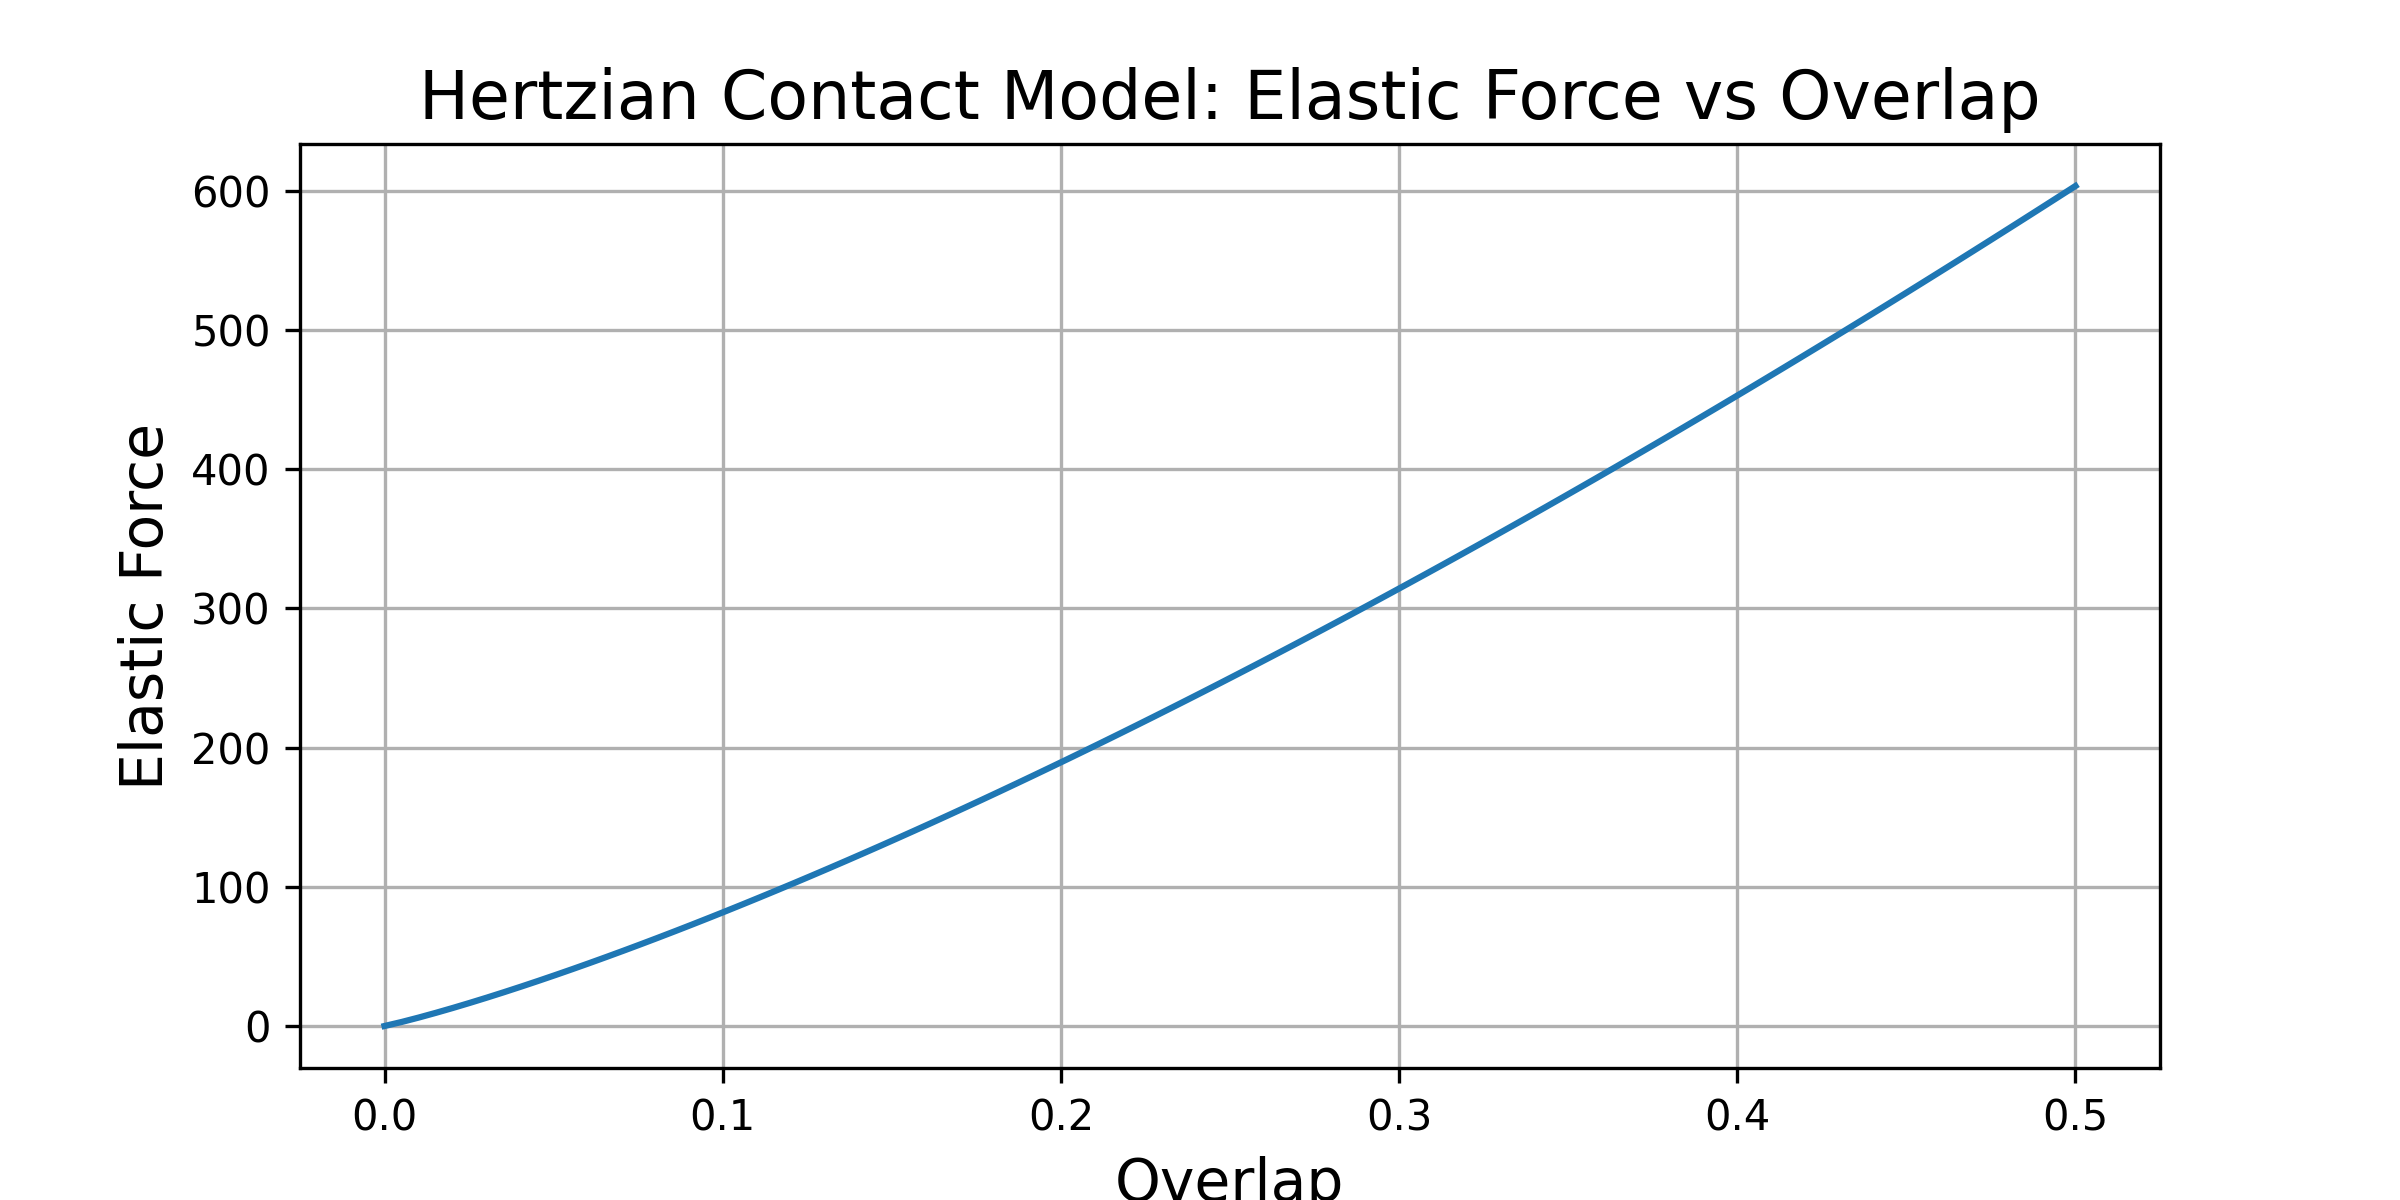
\includegraphics[width=\linewidth]{figures/hertzian_contact_model.png}
    \caption{Hertzian contact model. When two spherocylindrical cells overlap by a distance $\delta$, they experience a repulsive elastic force $\mathbf{F}^{\text{elastic}}$. The force acts along the normal vector $\hat{\mathbf{n}}$ at the contact point.}
    \label{fig:hertzian_contact_model}
\end{figure}

\subsection{Hard Collision Model}

The hard collision model adapted from Weady et al.~\cite{Weady2024SM} enforces strict non-overlapping constraints between cells using a constraint-based method. For each nearby cell pair, a constraint $\alpha$ is defined based on the closest points on their surfaces, $\mathbf{y}_n$ and $\mathbf{y}_m$. Unlike the soft model, which uses repulsive forces, the hard model determines contact forces via unknown scalar Lagrange multipliers $\gamma_\alpha$, which represent the magnitude of the impulse needed to prevent penetration.

The force on cell $n$ from constraint $\alpha$ is:
\begin{equation} \label{eq:constraint_force}
    \mathbf{F}^{\text{hard}}_{n\alpha} = \hat{\mathbf{n}}_\alpha \gamma_\alpha
\end{equation}

where $\hat{\mathbf{n}}_\alpha$ is the normal vector at the contact point. The total generalized force vector $\mathbfcal{F}$ for the colony depends linearly on the multipliers $\boldsymbol{\gamma} = [\dots, \gamma_\alpha, \dots]^\top \in \mathbb{R}^{C}$ and can be conveniently expressed in matrix form:
\begin{equation} \label{eq:force_as_function_of_multipliers}
    \mathbfcal{F}(\boldsymbol{\gamma}) = \mathbfcal{D} \boldsymbol{\gamma}
\end{equation}

where $\mathbfcal{D} \in \mathbb{R}^{6N \times C}$ is a sparse matrix consisting of contact normals and lever arms for all constraints. This matrix-vector product mimics the force assembly in ~\autoref{eq:force_assembly}, but uses the unknown multipliers $\boldsymbol{\gamma}$ instead of explicit force calculations. Similarly, the stress vector $\boldsymbol{\sigma} = [\dots, \sigma_n, \dots]^\top \in \mathbb{R}^{N}$ can also be expressed linearly in terms of $\boldsymbol{\gamma}$:
\begin{equation} \label{eq:stress_as_function_of_multipliers}
    \boldsymbol{\sigma}(\boldsymbol{\gamma}) = \mathbfcal{L} \boldsymbol{\gamma}
\end{equation}

where $\mathbfcal{L} \in \mathbb{R}^{N \times C}$ encodes stress contributions from each constraint, such that the matrix-vector product mimics the stress calculation in \autoref{eq:stress}. This also means that the growth rates $\dot{\boldsymbol{\ell}}$ depend (nonlinearly) on $\boldsymbol{\gamma}$ via \autoref{eq:growth}.

\subsubsection{Constraint Conditions}

To ensure that solving for the multipliers $\boldsymbol{\gamma}$ leads to physically meaningful results, three key conditions must be satisfied:


\begin{enumerate}
    \item \textbf{Repulsive Forces:} $\boldsymbol{\gamma} \geq \mathbf{0}$. This ensures that the forces are repulsive, preventing cells from attracting each other.
    \item \textbf{No-Overlap:} $\mathbf{\Phi}^{k+1} \geq \mathbf{0}$ with $\mathbf{\Phi}^{k+1} = [\dots, \Phi_\alpha^{k+1}, \dots]^\top$. Here, $\mathbf{\Phi}^{k+1} \in \mathbb{R}^{C}$ is the vector of signed separation distances between the pairs of cells associated with each constraint $\alpha$ at timestep $k+1$. Signed separation distances between cells are computed using the robust geometric algorithm described by~\cite{Yan2019, GeometricTools}.
          A positive value $\Phi_\alpha^{k+1}$ indicates that the cells in the next iteration are separated, while a negative value indicates overlap. This condition enforces that no overlaps occur after the update.
    \item \textbf{Complementarity Condition:}  $\boldsymbol{\gamma}^\top \mathbf{\Phi}^{k+1} = \mathbf{0}$ (often written as $\boldsymbol{\gamma} \perp \mathbf{\Phi}^{k+1}$). This condition enforces that if two cells are in contact in the next iteration (i.e., $\Phi_\alpha^{k+1} = 0$), then a force may act in the current iteration to prevent overlap.
          Conversely, if two cells are separated in the next iteration (i.e., $\Phi_\alpha^{k+1} > 0$), no force should act in the current iteration (i.e., $\gamma_\alpha = 0$) in order to avoid force application at a distance.
\end{enumerate}

These conditions are often abbreviated as:
\begin{equation}
    \mathbf{0} \leq \boldsymbol{\gamma} \perp \mathbf{\Phi}^{k+1} \geq \mathbf{0}.
\end{equation}


The colony update rule and additional conditions combine to form a system where the future state $\mathbfcal{C}^{k+1}$ and $\boldsymbol{\ell}^{k+1}$, and thus $\mathbf{\Phi}^{k+1}$ depend on $\boldsymbol{\gamma}$:
\begin{equation} \label{eq:colony_update_with_constraints}
    \begin{split}
        \mathbfcal{C}^{k+1} & = \mathbfcal{C}^k + \Delta t \mathbfcal{G}^k \mathbfcal{M}^k \mathbfcal{F}(\boldsymbol{\gamma})  \\
        \boldsymbol{\ell}^{k+1} & = \boldsymbol{\ell}^k + \Delta t \, \dot{\boldsymbol{\ell}}(\boldsymbol{\gamma}) \\
        \text{s.t.} \quad & \mathbf{0} \leq \boldsymbol{\gamma} \perp \mathbf{\Phi}^{k+1}(\boldsymbol{\gamma}) \geq \mathbf{0}.
    \end{split}
\end{equation}

\subsubsection{Linearization of the Constraint Condition}

The central challenge is that $\mathbf{\Phi}^{k+1}(\boldsymbol{\gamma})$ is a nonlinear function of the updated state $\mathbfcal{C}^{k+1}$ and the updated lengths $\boldsymbol{\ell}^{k+1}$, and is non-trivial to compute directly. Weady et al.~\cite{Weady2024SM} propose a linearization approach to approximate $\mathbf{\Phi}^{k+1}(\boldsymbol{\gamma})$ using a Taylor expansion around the current state $\mathbfcal{C}^k$ and lengths $\boldsymbol{\ell}^k$.

\noindent The change in $\mathbf{\Phi}$ in our model arises from two main effects:

\begin{enumerate}
    \item \textbf{Cell Motion:} All cell distances change due to the motion driven by collision forces. This is captured by the term $\dot{\mathbf{\Phi}^k}_{\text{motion}} = \frac{d \mathbf{\Phi}^k}{d \mathbfcal{C}} \frac{d \mathbfcal{C}}{dt} = (\nabla_{\mathbfcal{C}} \mathbf{\Phi}^k) \dot{\mathbfcal{C}}$.
    \item \textbf{Cell Growth:} Additionally, the cells grow, which affects separation according to $\dot{\mathbf{\Phi}^k}_{\text{growth}} = \frac{d \mathbf{\Phi}^k}{d \boldsymbol{\ell}} \frac{d \boldsymbol{\ell}}{dt} =-(\nabla_{\boldsymbol{\ell}} \mathbf{\Phi}^k) \dot{\boldsymbol{\ell}}$. The negative sign arises because as cells elongate, they reduce the separation distance between them.
\end{enumerate}

\noindent Combining these two effects leads to the following approximation for $\mathbf{\Phi}^{k+1}$:

\begin{equation}\label{eq:phi_expanded}
    \small
    \begin{split}
        \mathbf{\Phi}^{k+1}(\boldsymbol{\gamma}) & \approx \mathbf{\Phi}^k + \Delta t \left( \dot{\mathbf{\Phi}}_{\text{motion}} + \dot{\mathbf{\Phi}}_{\text{growth}} \right)\\
        & = \mathbf{\Phi}^k + \Delta t \left( (\nabla_{\mathbfcal{C}} \mathbf{\Phi}^k) \dot{\mathbfcal{C}}^k - (\nabla_{\boldsymbol{\ell}} \mathbf{\Phi}^k) \dot{\boldsymbol{\ell}} \right)\\
        & = \mathbf{\Phi}^k + \Delta t \left( (\nabla_{\mathbfcal{C}} \mathbf{\Phi}^k) \mathbfcal{G}^k \mathbfcal{M}^k  \mathbfcal{F}(\boldsymbol{\gamma}) - (\nabla_{\boldsymbol{\ell}} \mathbf{\Phi}^k) \dot{\boldsymbol{\ell}} \right)\\
        & \overset{\dagger}{=}
        \mathbf{\Phi}^k + \Delta t \left( \mathbfcal{D}^\top \mathbfcal{M}^k  \mathbfcal{F}(\boldsymbol{\gamma})
        - (\nabla_{\boldsymbol{\ell}} \mathbf{\Phi}^k) \dot{\boldsymbol{\ell}} \right)\\
        & \overset{\ddagger}{=} \mathbf{\Phi}^k + \Delta t \left( \mathbfcal{D}^\top \mathbfcal{M}^k \mathbfcal{D} \boldsymbol{\gamma} - \mathbfcal{L}^\top \left(\frac{\boldsymbol{\ell}}{\tau} \odot e^{-\lambda \mathbfcal{L} \boldsymbol{\gamma}} \right)\right)
    \end{split}
\end{equation}

\noindent where $\odot$ denotes the element-wise product.

Here $(\dagger)$, we use the previously introduced $\mathbfcal{D}$, noting that $\mathbfcal{D}^\top = (\nabla_{\mathbfcal{C}} \mathbf{\Phi}^k) \mathbfcal{G}^k$. The transpose $\mathbfcal{D}^\top$ can thus be interpreted as a Jacobian mapping velocities in $\mathbb{R}^{6N}$ first to changes in the colony state (via $\mathbfcal{G}^k$) and then to changes in the signed distance functions $\mathbf{\Phi}$ (see~\cite{Weady2024SM, Tasora2008} for details).

Similarly, in $(\ddagger)$, the previously defined $\mathbfcal{L}$, which encodes stress contributions from each constraint, has a transpose $\mathbfcal{L}^\top$ that maps stress-induced changes in cell lengths $\boldsymbol{\ell}$ to variations in $\mathbf{\Phi}$ (see~\cite{Weady2024SM} for details).

\subsubsection{Nonlinear Complementarity Problem}

Substituting the approximation of $\mathbf{\Phi}^{k+1}(\boldsymbol{\gamma})$ from \autoref{eq:phi_expanded} into the constraint conditions of \autoref{eq:colony_update_with_constraints} yields a nonlinear complementarity problem (NCP) for $\boldsymbol{\gamma}$ which no longer depends on the unknown future states $\mathbfcal{C}^{k+1}(\boldsymbol{\gamma})$ and $\boldsymbol{\ell}^{k+1}(\boldsymbol{\gamma})$:

\begin{empheq}[box=\fbox]{equation} \label{eq:ncp_boxed}
    \small
    \begin{aligned}
         & \text{Find } \boldsymbol{\gamma} \ \text{such that} \\
         & \mathbf{0} \leq \boldsymbol{\gamma} \perp
        \mathbf{\Phi}^k
        + \Delta t \left(
        \mathbfcal{D}^\top \mathbfcal{M}^k \mathbfcal{D} \boldsymbol{\gamma}
        - \mathbfcal{L}^\top
        \left(  \frac{\boldsymbol{\ell}}{\tau} \odot
            e^{-\lambda \mathbfcal{L}\boldsymbol{\gamma}}
            \right) \right) \ge \mathbf{0}.
    \end{aligned}
\end{empheq}


\subsubsection{Energy Minimization Solution}

To solve this nonlinear complementarity problem efficiently, we reframe it as an optimization problem using a special energy function $E(\boldsymbol{\gamma})$ whose minimization under non-negativity constraints resolves the contact forces~\cite{CellModellerMaths}. Physically, $E(\boldsymbol{\gamma})$ represents the work done by the contact forces and the system's internal energy:

\begin{equation} \label{eq:energy_function}
    \small
    \begin{aligned}
        \min_{\boldsymbol{\gamma} \geq \mathbf{0}}
        E(\boldsymbol{\gamma})
        =   \min_{\boldsymbol{\gamma} \geq \mathbf{0}} \;  \boldsymbol{\gamma}^\top \mathbf{\Phi}^k
         & +  \frac{\Delta t}{2}\, \boldsymbol{\gamma}^\top \mathbfcal{D}^\top \mathbfcal{M}^k \mathbfcal{D}\, \boldsymbol{\gamma} \\
         & + \mathbf{1}^\top \frac{\Delta t}{\lambda}
        \left( \frac{\boldsymbol{\ell}}{\tau} \odot e^{-\lambda\, \mathbfcal{L}\, \boldsymbol{\gamma}} \right)
    \end{aligned}
\end{equation}

By construction, the gradient of this energy equals the linearized separation distances $\mathbf{\Phi}^{k+1}(\boldsymbol{\gamma})$ from \autoref{eq:phi_expanded}:
\begin{equation}
    \small
    \begin{split}
        \nabla_{\boldsymbol{\gamma}} E & = \boldsymbol{\Phi}^k + \Delta t \left( \mathbfcal{D}^\top \mathbfcal{M}^k \mathbfcal{D} \boldsymbol{\gamma} - \mathbfcal{L}^\top \left( \frac{\boldsymbol{\ell}}{\tau} \odot e^{-\lambda \mathbfcal{L} \boldsymbol{\gamma}} \right)  \right) \\
        & = \boldsymbol{\Phi}^{k+1}(\boldsymbol{\gamma})
    \end{split}
\end{equation}

Because $E(\boldsymbol{\gamma})$ is convex, it has a single, global minimum. We compute this minimum using a projected gradient method, which iteratively takes steps in the direction of the negative gradient and projects the result onto the feasible set $\boldsymbol{\gamma} \geq 0$ to enforce repulsive forces.

At the solution, the Karush-Kuhn-Tucker (KKT) conditions for this constrained minimum are exactly equivalent to our physical constraints:

\begin{enumerate}
    \item \textbf{Primal feasibility} ($\boldsymbol{\gamma}^* \geq 0$): We enforce this explicitly through a projection (\texttt{max} operator) during minimization, which prevents forces from becoming attractive. Physically, this ensures that contact forces only push cells apart according to the \textbf{Repulsive Forces} constraint.

    \item \textbf{Dual feasibility} ($\nabla E(\boldsymbol{\gamma}^*) \geq 0$): At the solution $\boldsymbol{\gamma}^*$, the directional derivative of the energy must be non-negative in every feasible direction. A negative partial derivative would indicate that the energy could be reduced by increasing $\gamma_\alpha$, contradicting the optimality of $\boldsymbol{\gamma}^*$. Given the identity $\nabla E(\boldsymbol{\gamma}^*) = \boldsymbol{\Phi}^{k+1}(\boldsymbol{\gamma}^*)$, this condition ensures $\boldsymbol{\Phi}^{k+1} \geq 0$, enforcing the \textbf{No-Overlap} constraint.

    \item \textbf{Complementary slackness} ($\boldsymbol{\gamma}^{*\top} \boldsymbol{\Phi}^{k+1} = 0$): This condition holds for a similar reason. Since both $\boldsymbol{\gamma}^* \geq 0$ and $\boldsymbol{\Phi}^{k+1} \geq 0$ at the solution, their product can only be zero if at least one term is zero for each contact. If a contact force is active ($\gamma_\alpha > 0$), it means the system is free to adjust this force to find the minimum. At the true minimum, there can be no direction left to lower the energy. Therefore, for a non-zero force to be part of the final, optimal solution, the gradient (which equals $\Phi^{k+1}_\alpha$) must be zero at that point. Conversely, if $\gamma_\alpha = 0$, the gradient can be positive ($\Phi^{k+1}_\alpha \geq 0$) because the energy cannot be lowered by making $\gamma_\alpha$ more negative (as it is forbidden by the Repulsive Forces constraint). Thus, the product $\gamma_\alpha \Phi^{k+1}_\alpha = 0$ for each contact $\alpha$, leading to the overall complementary slackness condition. Physically, this means forces act only where cells are touching. Separated cells never experience any repulsive force, satisfying the \textbf{Complementarity Condition}.
\end{enumerate}

Thus, the unique global minimizer $\boldsymbol{\gamma}^*$ resolves all contacts according to the physical laws of rigid-body interactions. This equivalence between the KKT conditions of a convex optimization problem and a complementarity problem is a well-known result in optimization theory~\cite{Nocedal2006} and is widely used in constraint-based physics simulations~\cite{Yan2022,Tasora2008, Yan2019, Li2021, Weady2024SM,Rudge2012,Macklin2014,Ferguson2021,CellModellerMaths}.

\subsubsection{Numerical Solution}

We solve the constrained optimization problem using the Barzilai-Borwein projected gradient descent method (BBPGD)~\cite{BBPGD}, implemented as in~\cite{Weady2024SM,Yan2019}. This method is well-suited to large-scale problems due to its computational efficiency and scalability. The solver iterates until convergence, yielding the optimal contact forces $\boldsymbol{\gamma}^*$, which are then used to compute $\mathbfcal{F}(\boldsymbol{\gamma}^*)$ and $\dot{\boldsymbol{\ell}}(\boldsymbol{\gamma}^*)$ for updating the colony state via \autoref{eq:colony_update}.

Following Weady et al.~\cite{Weady2024SM}, we adopt a convergence criterion based on a residual that directly measures physical overlap. The solver terminates when this residual falls below a user-specified tolerance of $\epsilon = d/500 = 0.5/500 = 10^{-3}$, ensuring that the maximum overlap between any pair of cells remains below $0.1\%$ of the cell diameter $d = 0.5$.

\subsubsection{Limitations of the Linearization}

A fundamental limitation of the linearization is that orthogonal motions, specifically rotations about contact points and translations parallel to the contact plane, are unconstrained within the linear approximation~\cite{Weady2024SM}. Consequently, even after the BBPGD algorithm converges to the specified tolerance $\epsilon$, residual overlaps may still be present that violate the non-overlap constraint.

To address this limitation, Weady et al.~\cite{Weady2024SM} developed the recursively generated linear complementarity problem (ReLCP) method. After each BBPGD convergence, ReLCP identifies any remaining overlaps by examining all pairwise cell distances, generates new constraints for these violations, and re-solves the complementarity problem with the augmented constraint set. This process iterates until all cell overlaps fall below the tolerance $\epsilon$. This hierarchical approach ensures that the non-overlap condition is strictly enforced, even in the presence of complex contact geometries and coupled motions (see \autoref{fig:bbpgd_residual}). The iterative refinement procedure typically converges within a small number of iterations, making it computationally tractable for most simulations~\cite{Weady2024SM}.

Nevertheless, this approach still requires a sufficiently small timestep, $\Delta t \sim 5 \times 10^{-4}$ h (see \autoref{fig:simulation_time_vs_dt}), to prevent excessive cell motion~\cite{Yan2022}. If cells move too far in a single timestep, new overlaps can form that the linearization does not capture, preventing constraint resolution. In practice, this can cause the BBPGD method to fail to converge or the ReLCP solver to be unable to resolve all overlaps within a reasonable number of iterations, leading to simulation failure.

Despite this computational restriction, the hard model's timestep requirement is less severe than the soft model's, though it still represents a significant computational bottleneck for large colonies with millions of cells.

\section{Implementation}

All simulations in this paper were performed with a custom C++ framework designed for large-scale simulations of proliferating cell collectives. The framework leverages distributed-memory parallel computing and standard HPC libraries to achieve scalability, enabling simulations of hundreds of thousands of cells across hundreds of CPU cores. The implementation combines concepts from Weady et al.~\cite{Weady2024SM} and similar frameworks~\cite{Tasora2008,Yan2019}.

\subsection{Distributed Computing Architecture}

The core architecture is built on two foundational libraries:
\begin{itemize}
    \item \textbf{PETSc}~\cite{petsc-web-page}: Used as a backend for distributed vectors and sparse matrices. PETSc partitions data across MPI processes and transparently handles inter-process communication for global operations (e.g., matrix-vector products and reductions).
    \item \textbf{MPI}: Underlies all inter-process communication, including ghost-cell exchanges at domain boundaries to maintain consistent collision handling across partitions.
\end{itemize}

Built on these abstractions, the framework implements the full physics pipeline, including both the ReLCP solver for the hard collision model and the soft collision model.

\subsection{Collision Handling Pipeline}

Collisions are processed through a unified pipeline designed to decouple geometry from physics. The process consists of two phases: broad-phase detection using a spatial grid (reducing neighbor searches to $O(N)$) and narrow-phase detection that computes exact contact points and geometric information. For each collision detected, the framework assembles a standardized data structure containing contact points, normals, and lever arms. This structure is passed to either the hard or soft collision model, which computes the resulting forces and torques. This abstraction allows seamless switching between collision models without altering the overall simulation flow.

Each collision detector call generates a single constraint per neighboring cell-pair within a threshold distance $d = 0.5$. As this threshold is larger than zero, it captures both overlapping and closely adjacent cells. This overapproximation is crucial for the stability of the hard model. For the soft model, those non-overlapping cell-pairs contribute no forces (since $\delta < 0$), while for the hard model they provide additional global information that improves constraint resolution. Ideally, constraints would be constructed between all cell pairs regardless of distance, but for computational efficiency only nearby cells are considered~\cite{Yan2019, Yan2022}.

\subsection{Adaptive Timestepping}

To enhance stability and convergence, particularly for fast-moving cells that might overlap significantly within a timestep, we employ an adaptive timestepping scheme, allowing the timestep $\Delta t$ to vary dynamically based on the current state of the colony. To our knowledge, this approach has not been implemented in comparable engines.

The adaptive timestep strategy (outlined in \autoref{alg:adaptive_dt}) is based on the Courant-Friedrichs-Lewy (CFL) condition~\cite{Courant1928}, which provides a stability criterion linking temporal and spatial resolution:

\begin{equation}
    \text{CFL} = \frac{u \, \Delta t}{\Delta x} \leq C_{\text{max}}.
\end{equation}

For our cell-based system, we define a characteristic velocity scale $u_m$ as the median of all cell velocities (including growth rates) and a characteristic spatial scale $\Delta x$ as the solver tolerance $\varepsilon = 10^{-3}$, which controls the maximum allowable displacement per step. Enforcing that cells move no more than a fraction of $\varepsilon$ per timestep leads to the following expression for the adaptive timestep:

\begin{equation} \label{eq:cfl_dt}
    \Delta t = \frac{c \cdot\, \varepsilon}{u_m}
\end{equation}

where $c$ is a user-defined CFL number (we use $c = 0.5$, ensuring cells move at most half the tolerance per step). Choosing $\Delta t$ like this, ensures that most cells move less than half the solver tolerance in each timestep, preventing excessive overlaps that could destabilize the simulation.

\begin{algorithm}[H]
    \caption{Adaptive Timestep Control}
    \label{alg:adaptive_dt}
    \begin{algorithmic}[1]
        \Require Particle set $\{p_i\}$ with velocities $v_i$ and growth rates $\dot{\ell_i}$, current timestep $\Delta t$, solver tolerance $\varepsilon$, smoothing factor $\alpha$.
        \Ensure Updated timestep $\Delta t$.

        \State Compute characteristic velocity $u_i = \|v_i\| + \dot{\ell_i}$ for each particle.
        \State Calculate $u_m$ as the median of $\{u_i\}$.
        \State Determine $\Delta t^*$ using~\autoref{eq:cfl_dt}.
        \State Smooth the timestep change to avoid oscillations: $\Delta t_{\text{new}} = (1 - \alpha)\Delta t + \alpha \Delta t^*$ with $\alpha = 0.01$.
        \State Clamp $\Delta t_{\text{new}}$ within 20\% of current $\Delta t$ to prevent abrupt changes.
        \State Update simulation timestep: $\Delta t \gets \Delta t_{\text{new}}$.
    \end{algorithmic}
\end{algorithm}

\subsection{Simulation Output and Availability}

Simulation results are saved in VTK format for visualization with ParaView~\cite{ahrens2005paraview}. Cell attributes, including positions, orientations, lengths, stresses, growth rates and contact forces, are recorded at user-defined intervals. The framework also logs performance metrics, such as timestep sizes, solver iterations, and computation times, to facilitate analysis and debugging.

The full simulation framework, including all features and implementations described in this work, is openly available on GitHub at \url{https://github.com/manuellerchner/MicrobeGrowthSim-IDP}.

\newpage

\section{Pattern Formation Analysis}

\subsection{Concentric Ring Patterns}

We validate both implementations by reproducing concentric ring patterns that arise under stress-sensitive growth, as reported in~\cite{Weady2024}. As shown in \autoref{fig:pattern_formation}, both models successfully produce qualitatively similar ring structures, demonstrating that the core mechanics of growth and mechanical feedback are effectively captured by both collision handling approaches.

The effect of $\lambda$ on pattern formation is consistent across both models. At very low stress-sensitivity ($\lambda = 10^{-4}$), growth inhibition is too weak to generate significant stress gradients, and thus no rings form. At intermediate sensitivity ($\lambda = 10^{-3}$), distinct concentric rings emerge early in the simulation and persist as the colony expands, with ring spacing determined by the balance between growth and stress. At high sensitivity ($\lambda = 10^{-2}$), an initially formed ring quickly dissipates as cells reorient to random orientations and growth nearly ceases due to strong mechanical inhibition throughout most of the colony.

Despite these qualitatively similar outcomes, visual differences emerge between the models. The soft model produces visibly denser patterns with a fuzzy appearance due to allowable cell overlap, while the hard model yields sharper, more sparsely looking rings. Nevertheless, macroscopic features, such as the number of rings, spacing, and colony expansion rate, remain comparable between the two models.

\begin{figure*}[p]
    \centering

    % % Lambda = 10^-2 comparison

    Growth Comparison $\lambda=10^{-2}$
    \begin{tabular}{r M{0.2\textwidth} M{0.2\textwidth} M{0.2\textwidth} M{0.2\textwidth}}
        \growthcomparisonrow{hard}{e-2}{0055}{0100}{0150}{0199}
        \growthcomparisonrow{soft}{e-2}{0055}{0100}{0150}{0200}
    \end{tabular}
    % Lambda = 10^-3 comparison

    Growth Comparison $\lambda=10^{-3}$
    \begin{tabular}{r M{0.2\textwidth} M{0.2\textwidth} M{0.2\textwidth} M{0.2\textwidth}}
        \growthcomparisonrow{hard}{e-3}{0052}{0100}{0150}{0198}
        \growthcomparisonrow{soft}{e-3}{0048}{0110}{0149}{0187}
    \end{tabular}

    % Lambda = 10^-4 comparison

    Growth Comparison $\lambda=10^{-4}$
    \begin{tabular}{r M{0.2\textwidth} M{0.2\textwidth} M{0.2\textwidth} M{0.2\textwidth}}
        \growthcomparisonrow{hard}{e-4}{0051}{0100}{0140}{0192}
        \growthcomparisonrow{soft}{e-4}{0048}{0105}{0134}{0198}
    \end{tabular}

    \caption{Comparison of pattern formation between hard and soft collision models at similar colony sizes. Each row shows the colony evolutions up to a maximum colony radius of 100. The color indicates the length of the cells (short cells are darker, longer cells are lighter). Clear concentric ring patterns are visible for both models at $\lambda = 10^{-3}$ confirming the results from~\cite{Weady2024}.}
    \label{fig:pattern_formation}
\end{figure*}

\subsection{Cell Density and Local Packing Fraction}

The most striking difference between the models is the cell packing density (see \autoref{fig:dense_packing_comparison}). The soft model exhibits significantly denser packing in the colony center, decreasing radially outward (see \autoref{fig:radial_distribution_packing_fraction}). For very low stress-sensitivity ($\lambda = 10^{-4}$), local packing fractions reach values of 5, far exceeding the maximum possible for rigid spherocylinders. In contrast, the hard model maintains approximately constant, and physically realistic, packing density of 0.9 throughout the colony.

The unphysical packing fraction arises because the soft model relies on local pairwise forces that cannot fully propagate stress to the colony edge. Combined with a numerical timestep too large to resolve all collisions, this leads to excessive cell overlap and overcrowding in the interior. \autoref{fig:max_overlap_simulation} quantifies this effect: the soft model's maximum cell overlap steadily increases throughout the simulation, reaching nearly complete interpenetration by the end. In contrast, the hard model maintains maximum overlap near the solver tolerance $\epsilon = 10^{-3}$ by enforcing the strict non-overlap constraints.

A contributing factor to this excessive overlap is the adaptive timestep method (see \autoref{alg:adaptive_dt}), which bases $\Delta t$ solely on cell velocities but not on current overlap. Once cells begin overlapping, they can continue doing so as long as velocities remain low. A more sophisticated scheme could consider maximum overlap when adjusting $\Delta t$. Such an improvement is, however, beyond the scope of this work.

\begin{figure}[H]
    \centering
    \begin{subfigure}[b]{0.49\columnwidth}
        \centering
        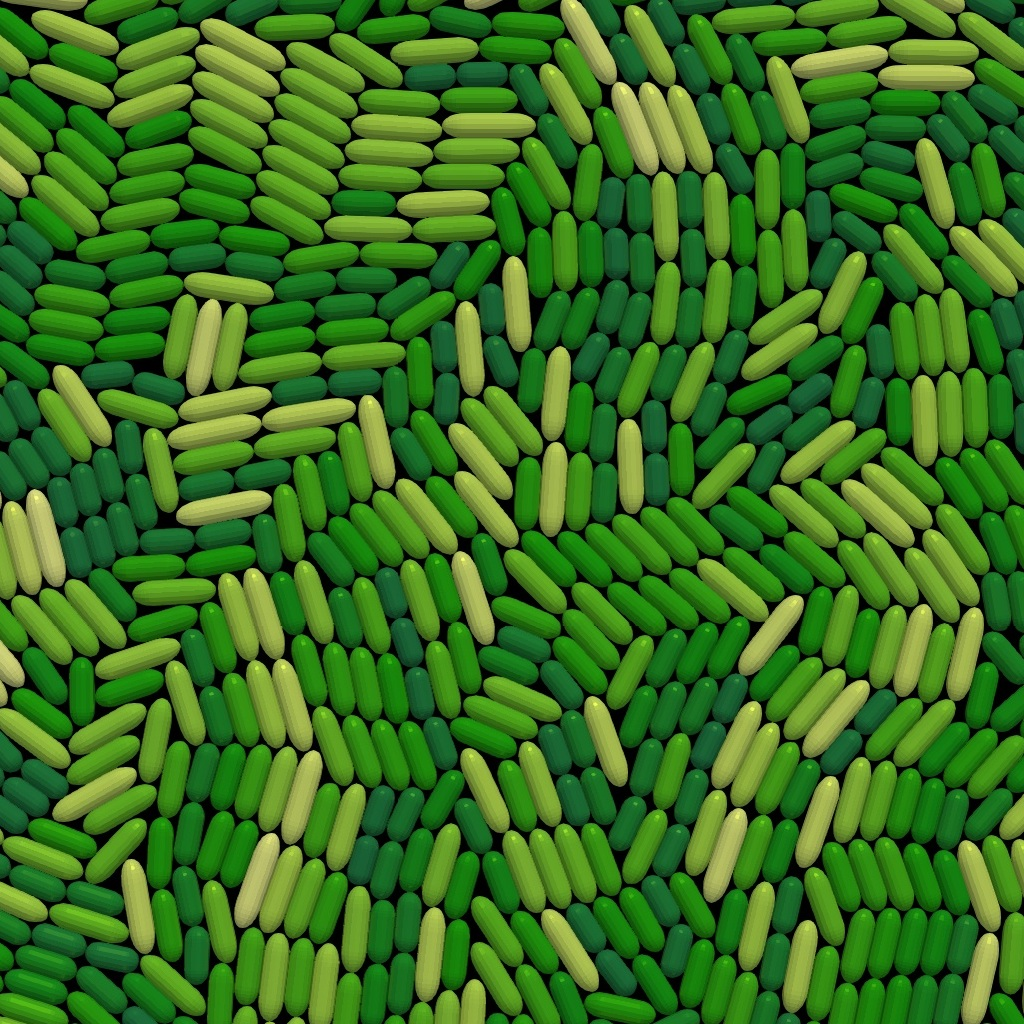
\includegraphics[width=\linewidth]{figures/comparison_plots/density_hard.jpeg}
        \caption{Hard model}
    \end{subfigure}
    \begin{subfigure}[b]{0.49\columnwidth}
        \centering
        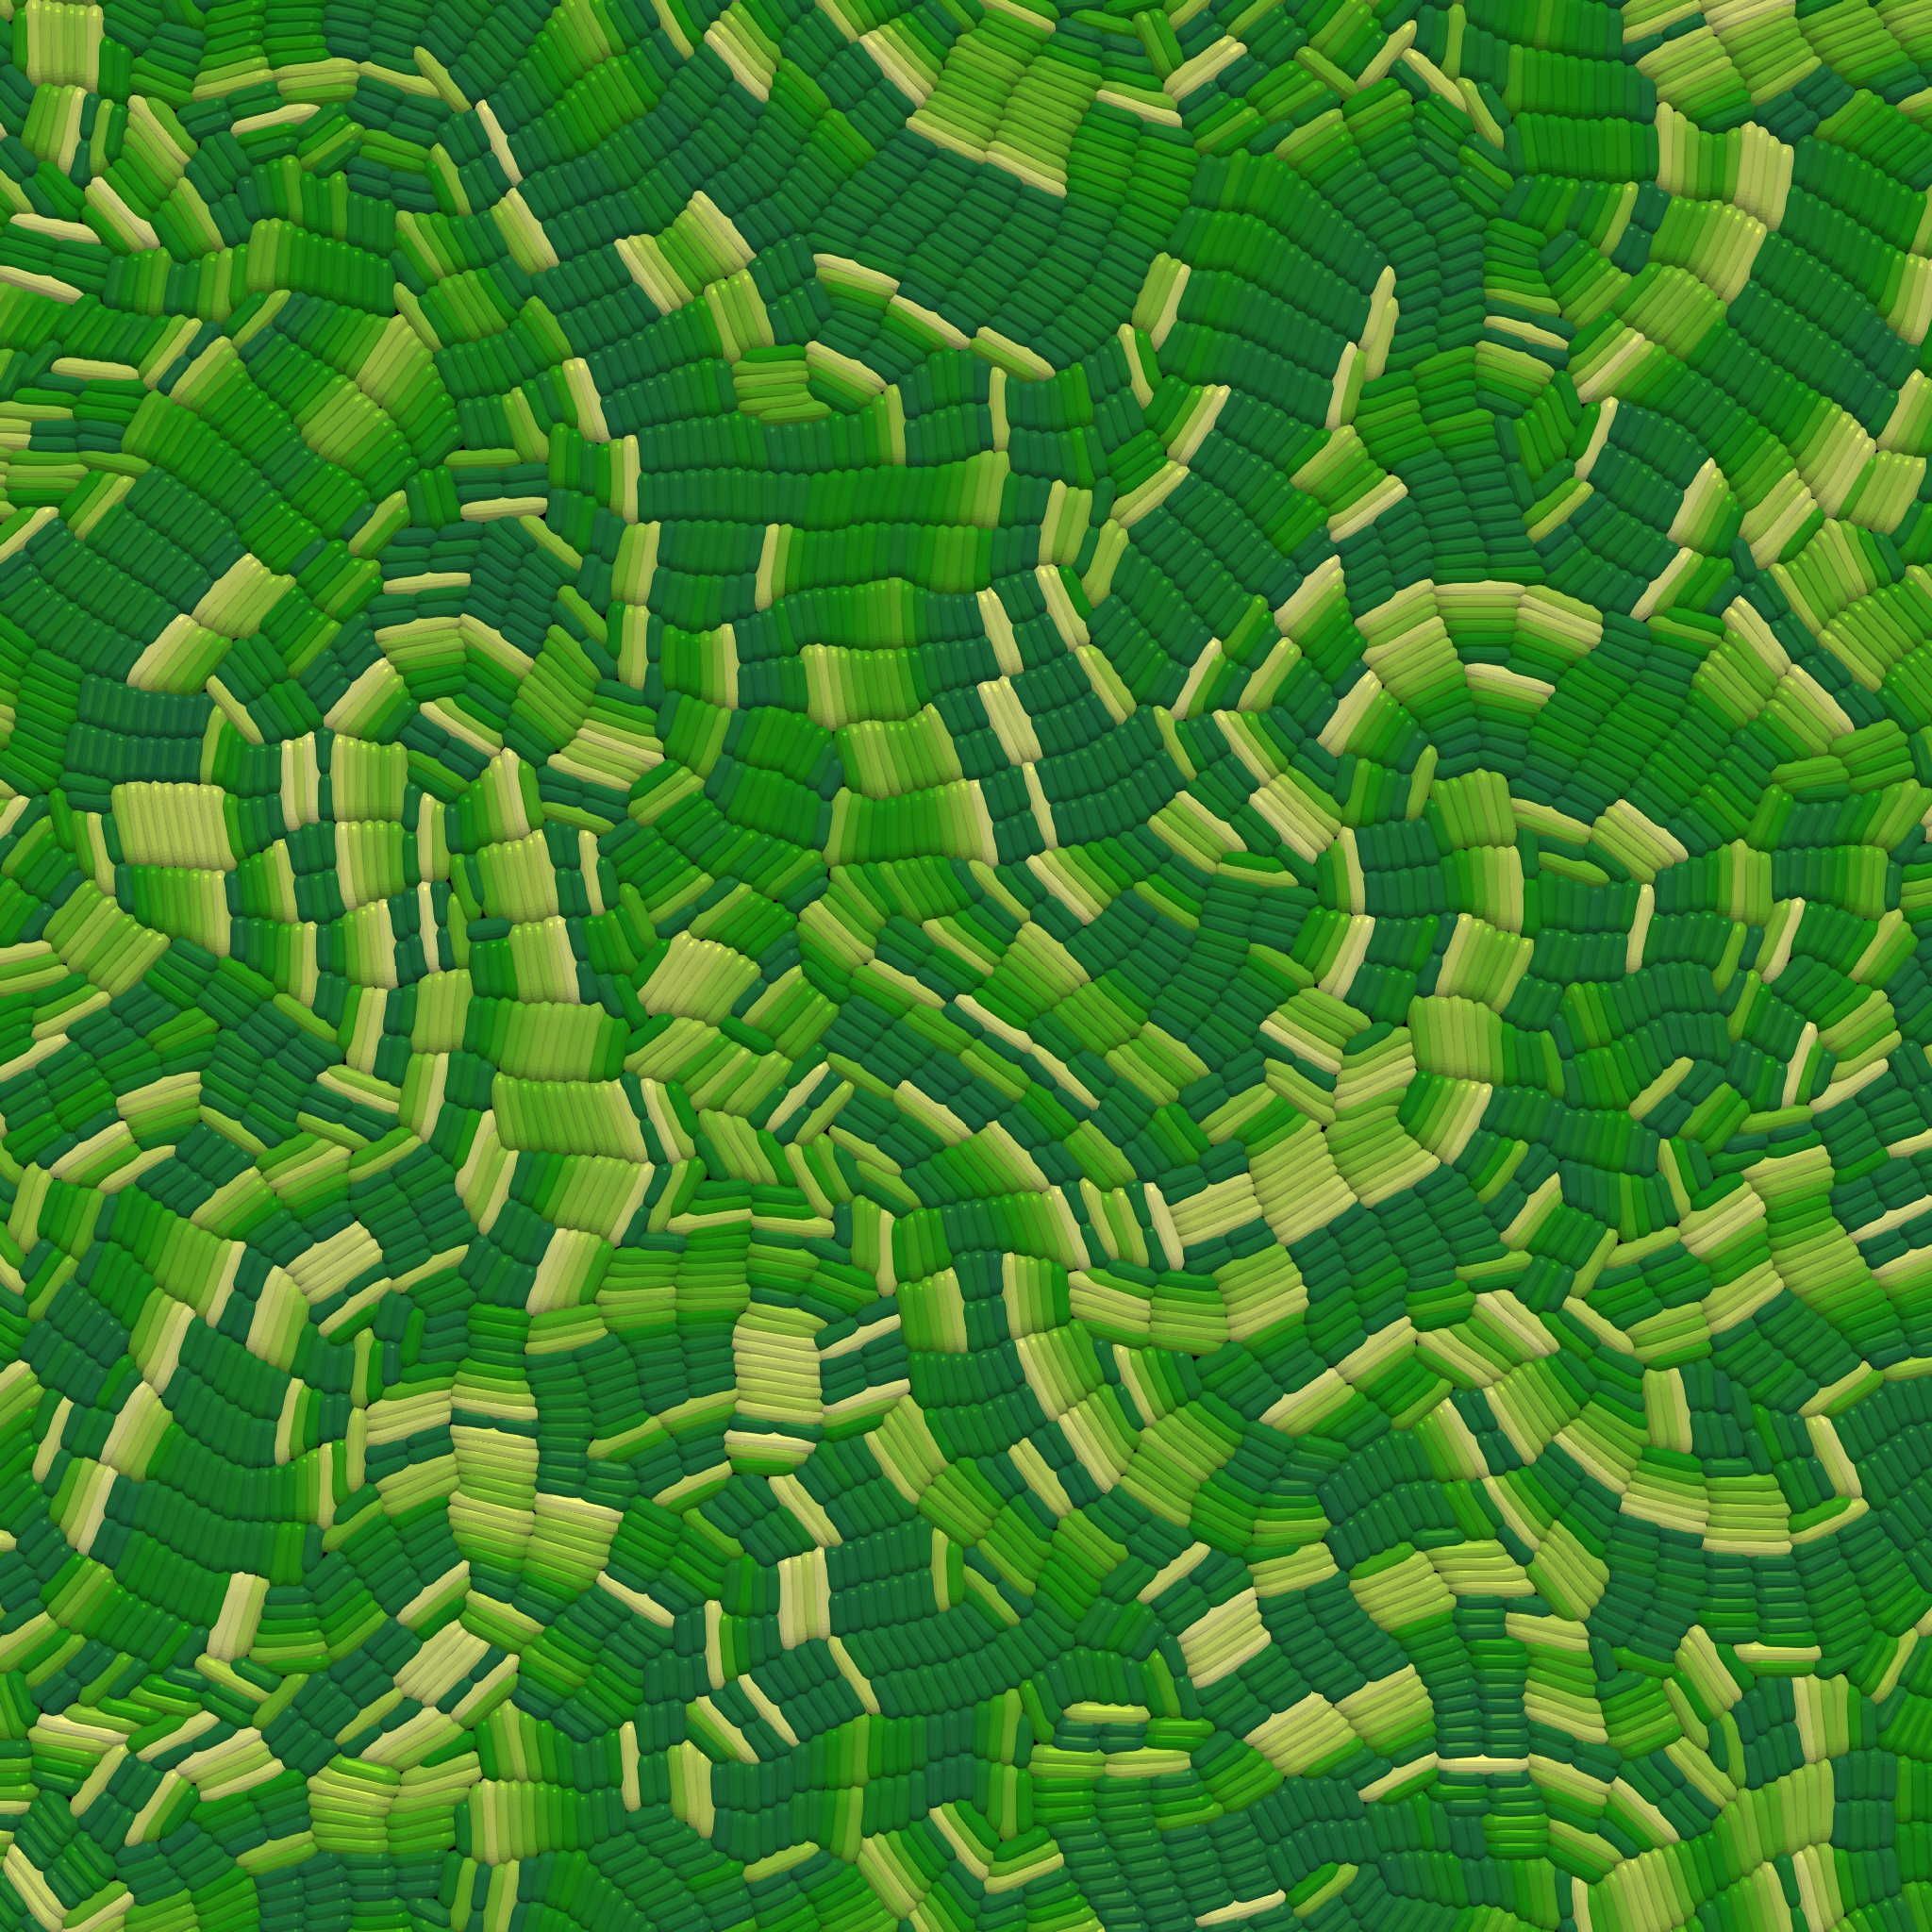
\includegraphics[width=\linewidth]{figures/comparison_plots/density_soft.jpeg}
        \caption{Soft model}
    \end{subfigure}
    \caption{Close-up comparison of cell packing in the colony center for both collision models. The hard model (a) maintains near-optimal packing, while the soft model (b) exhibits significant overlap and overcrowding.}
    \label{fig:dense_packing_comparison}
\end{figure}

\begin{figure}[H]
    \centering
    \begin{subfigure}[b]{\linewidth}
        \centering
        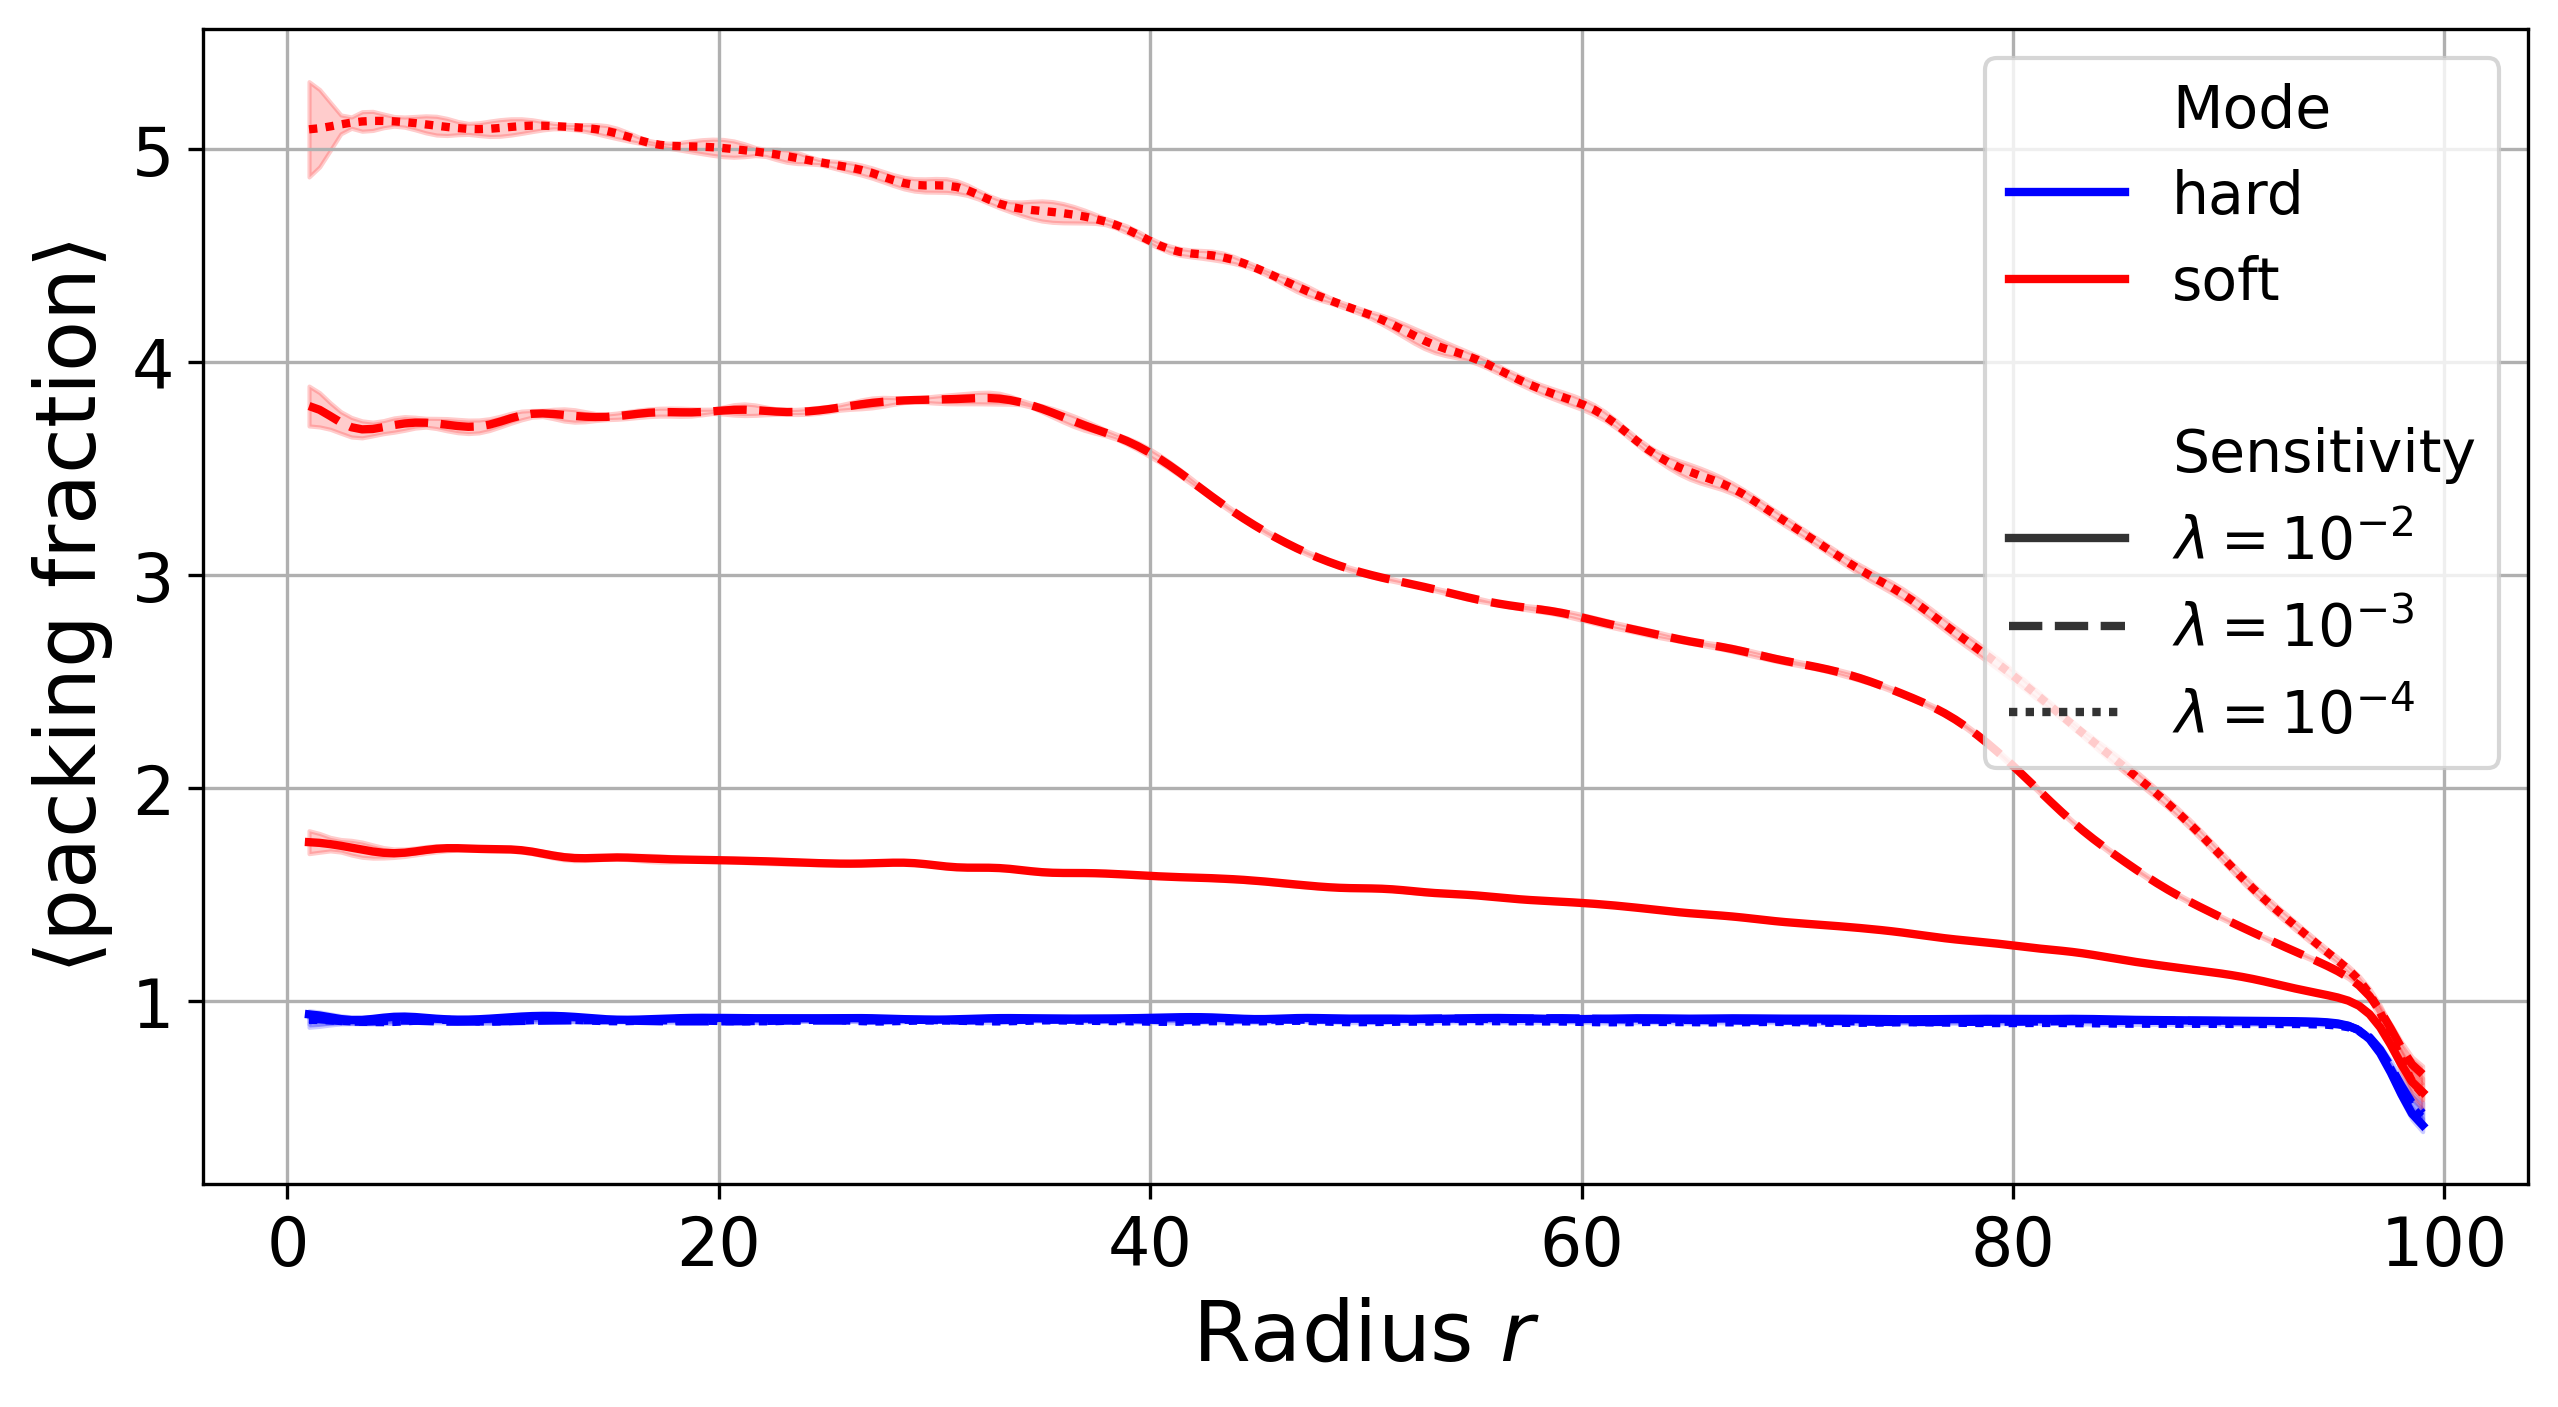
\includegraphics[width=\linewidth]{figures/comparison_plots/combined_radial_packing_fraction.png}
        \caption{Radial packing fraction profiles ($\phi = \frac{A_{\text{cells}}}{A_{\text{total}}}$) for both models. Here $A_{\text{cells}}$ is the total area occupied by cells within a radial bin of width 2 at distance $r$ from the colony center, and $A_{\text{total}}$ is the annular area of that bin. The hard model maintains nearly optimal packing, while the soft model exhibits higher fractions in the colony center.}
        \label{fig:radial_distribution_packing_fraction}
    \end{subfigure}

    \begin{subfigure}[b]{\linewidth}
        \centering
        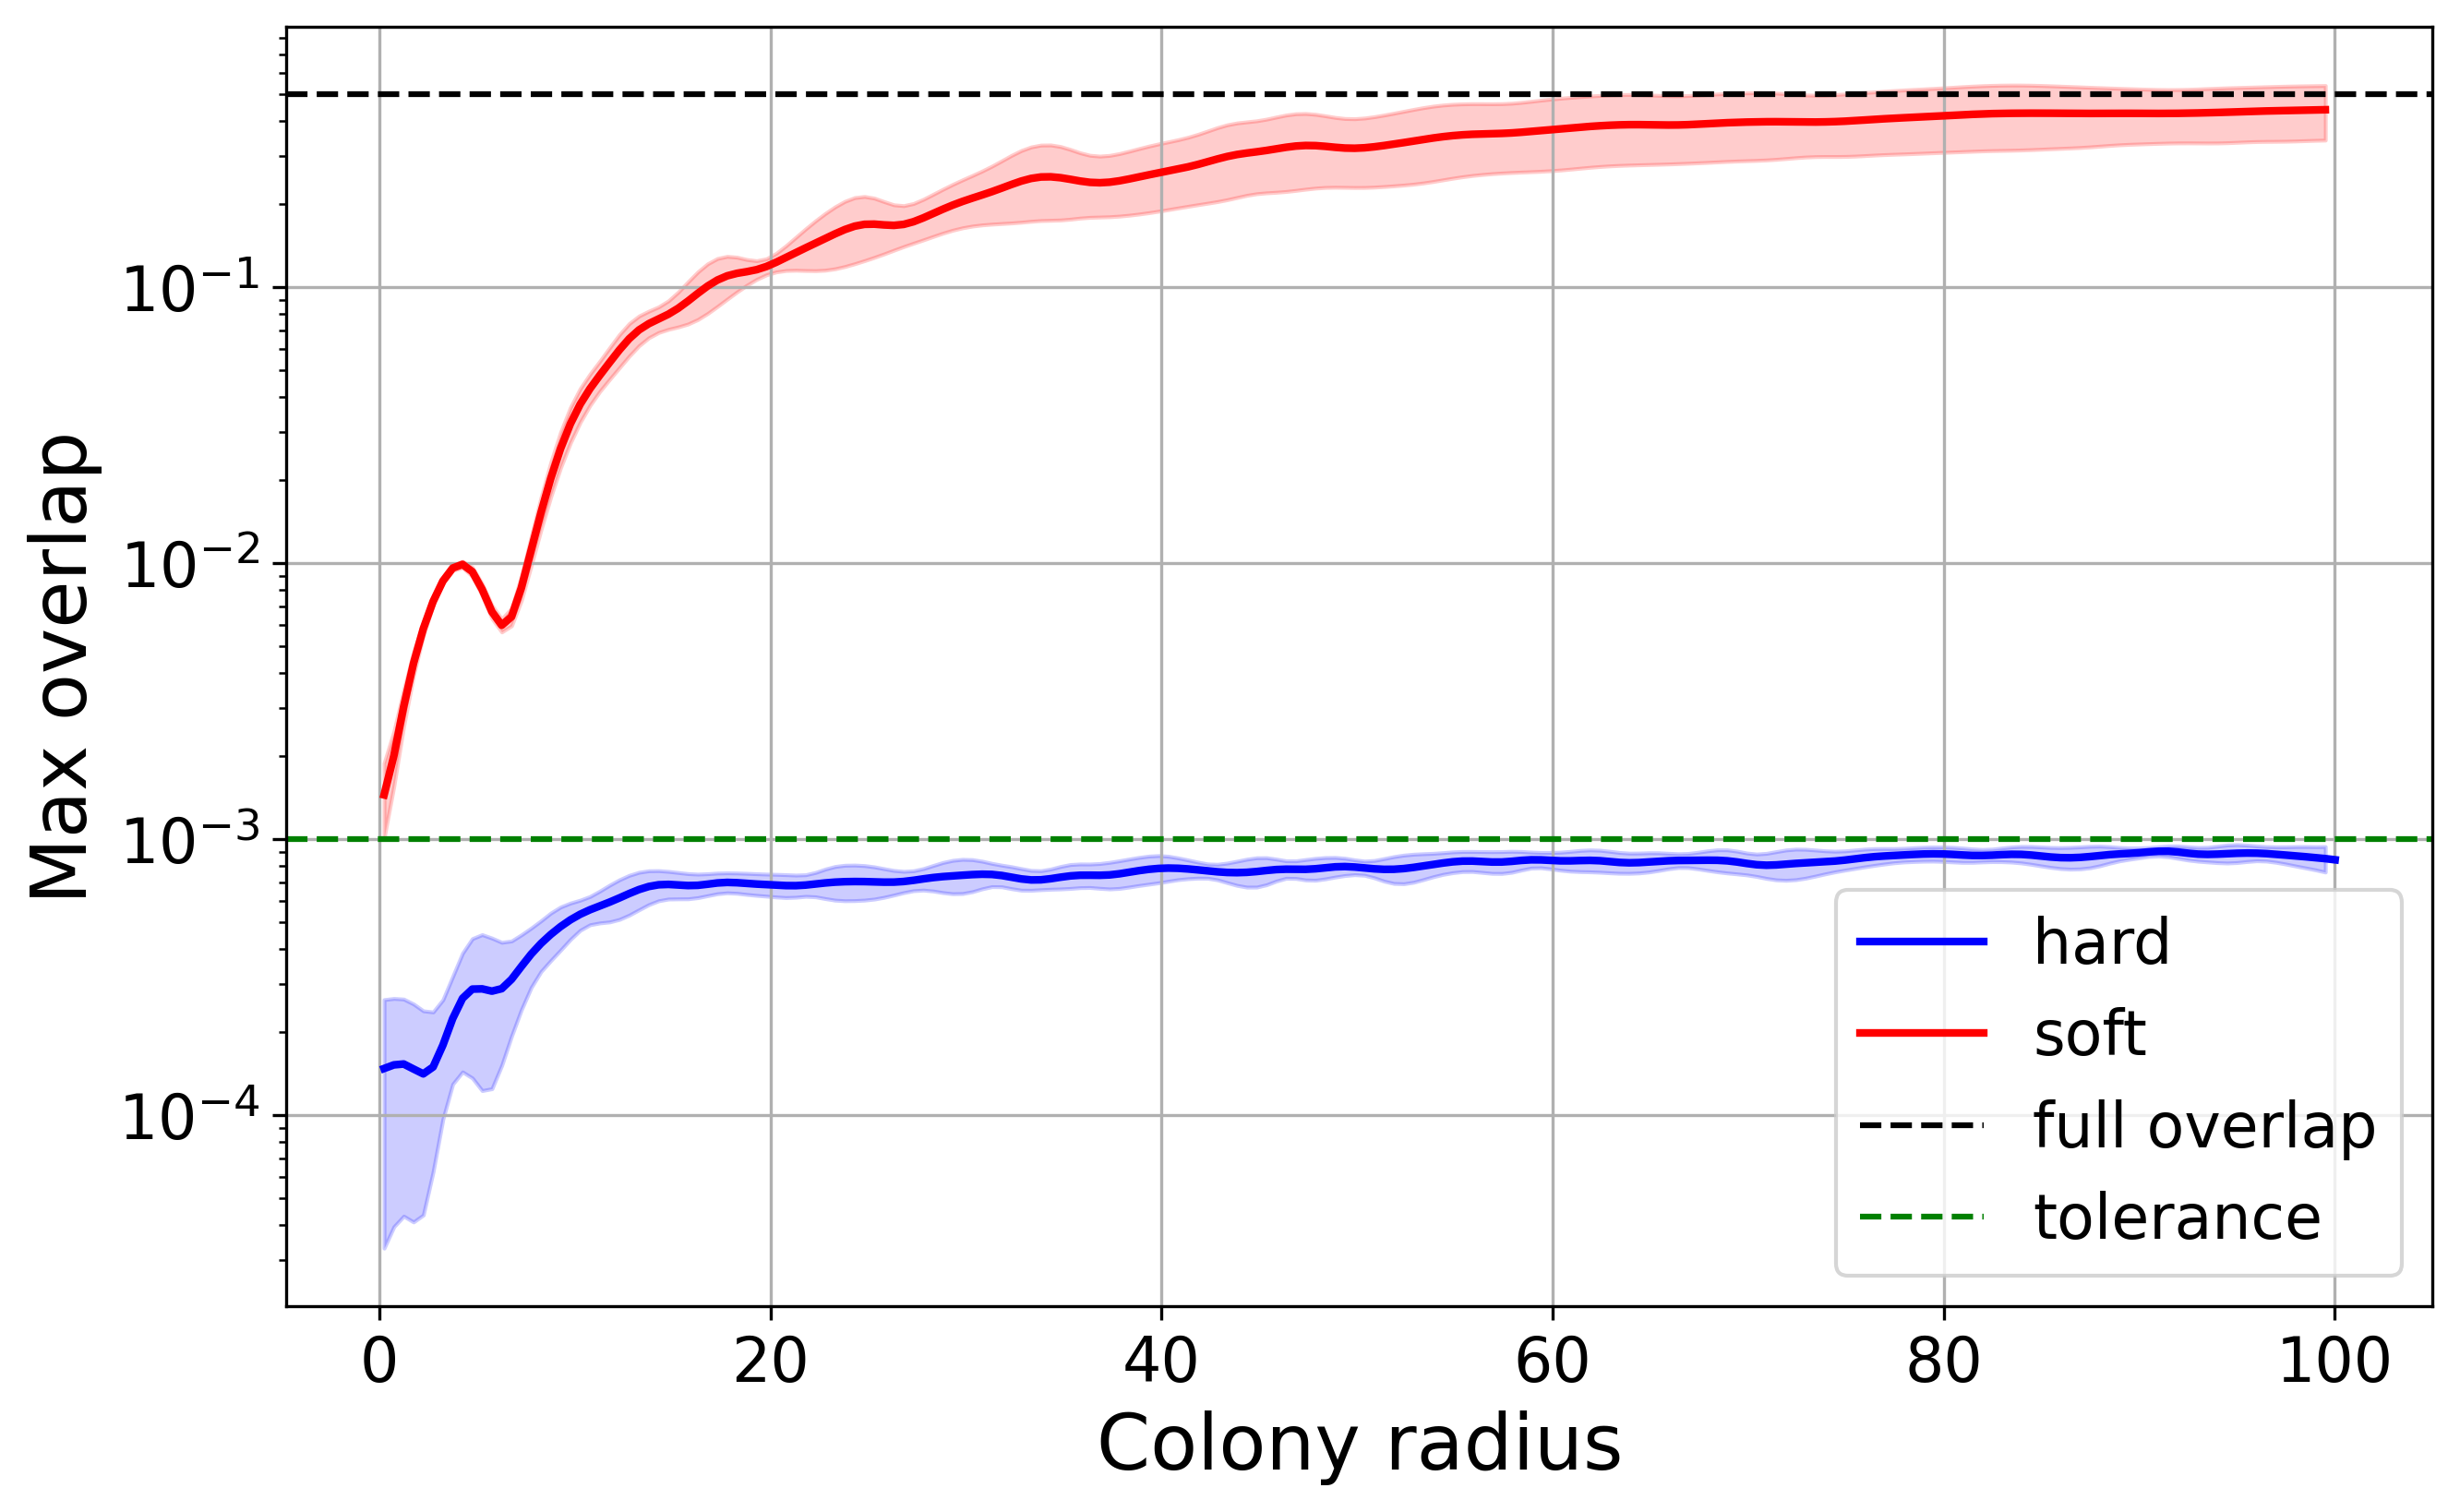
\includegraphics[width=\linewidth]{figures/comparison_plots/combined_colony_radius_vs_max_overlap_with_lines.png}
        \caption{Maximum cell overlap over simulation time. The hard model maintains overlap near the solver tolerance $\epsilon = 10^{-3}$, while the soft model exhibits a steady increase, reaching near-complete overlap by the simulation end.}
        \label{fig:max_overlap_simulation}
    \end{subfigure}

    \caption{Cell packing analysis comparing hard and soft collision models. (a) Radial packing fraction profiles. (b) Maximum cell overlap vs. colony growth.}
    \label{fig:combined_packing_analysis}
\end{figure}

\subsection{Colony Growth Dynamics and Number of Cells}
\label{sec:colony_growth_dynamics}

A direct consequence of the overcrowded interior in the soft model is its impact on the number of cells. The soft model requires significantly more cells to reach the same colony radius (see \autoref{fig:colony_radius_vs_num_cells}). At low stress-sensitivity ($\lambda = 10^{-4}$), where growth is largely decoupled from mechanical inhibition and cells multiply exponentially, the soft model requires almost three times as many cells as the hard model to reach the same radius. This disparity indicates that the overcrowded interior cannot effectively contribute to outward colony pressure and interior cells remain essentially immobile, while still growing and dividing, leading to a large excess of cells that do not aid expansion.

The computational consequences are substantial: the soft model requires simulating far more cells to reach the same colony size, directly increasing both memory usage and runtime. A detailed analysis of the impact on computational performance is presented in \autoref{sec:performance_analysis}.

\begin{figure}[h]
    \centering
    \begin{subfigure}[b]{\linewidth}
        \centering
        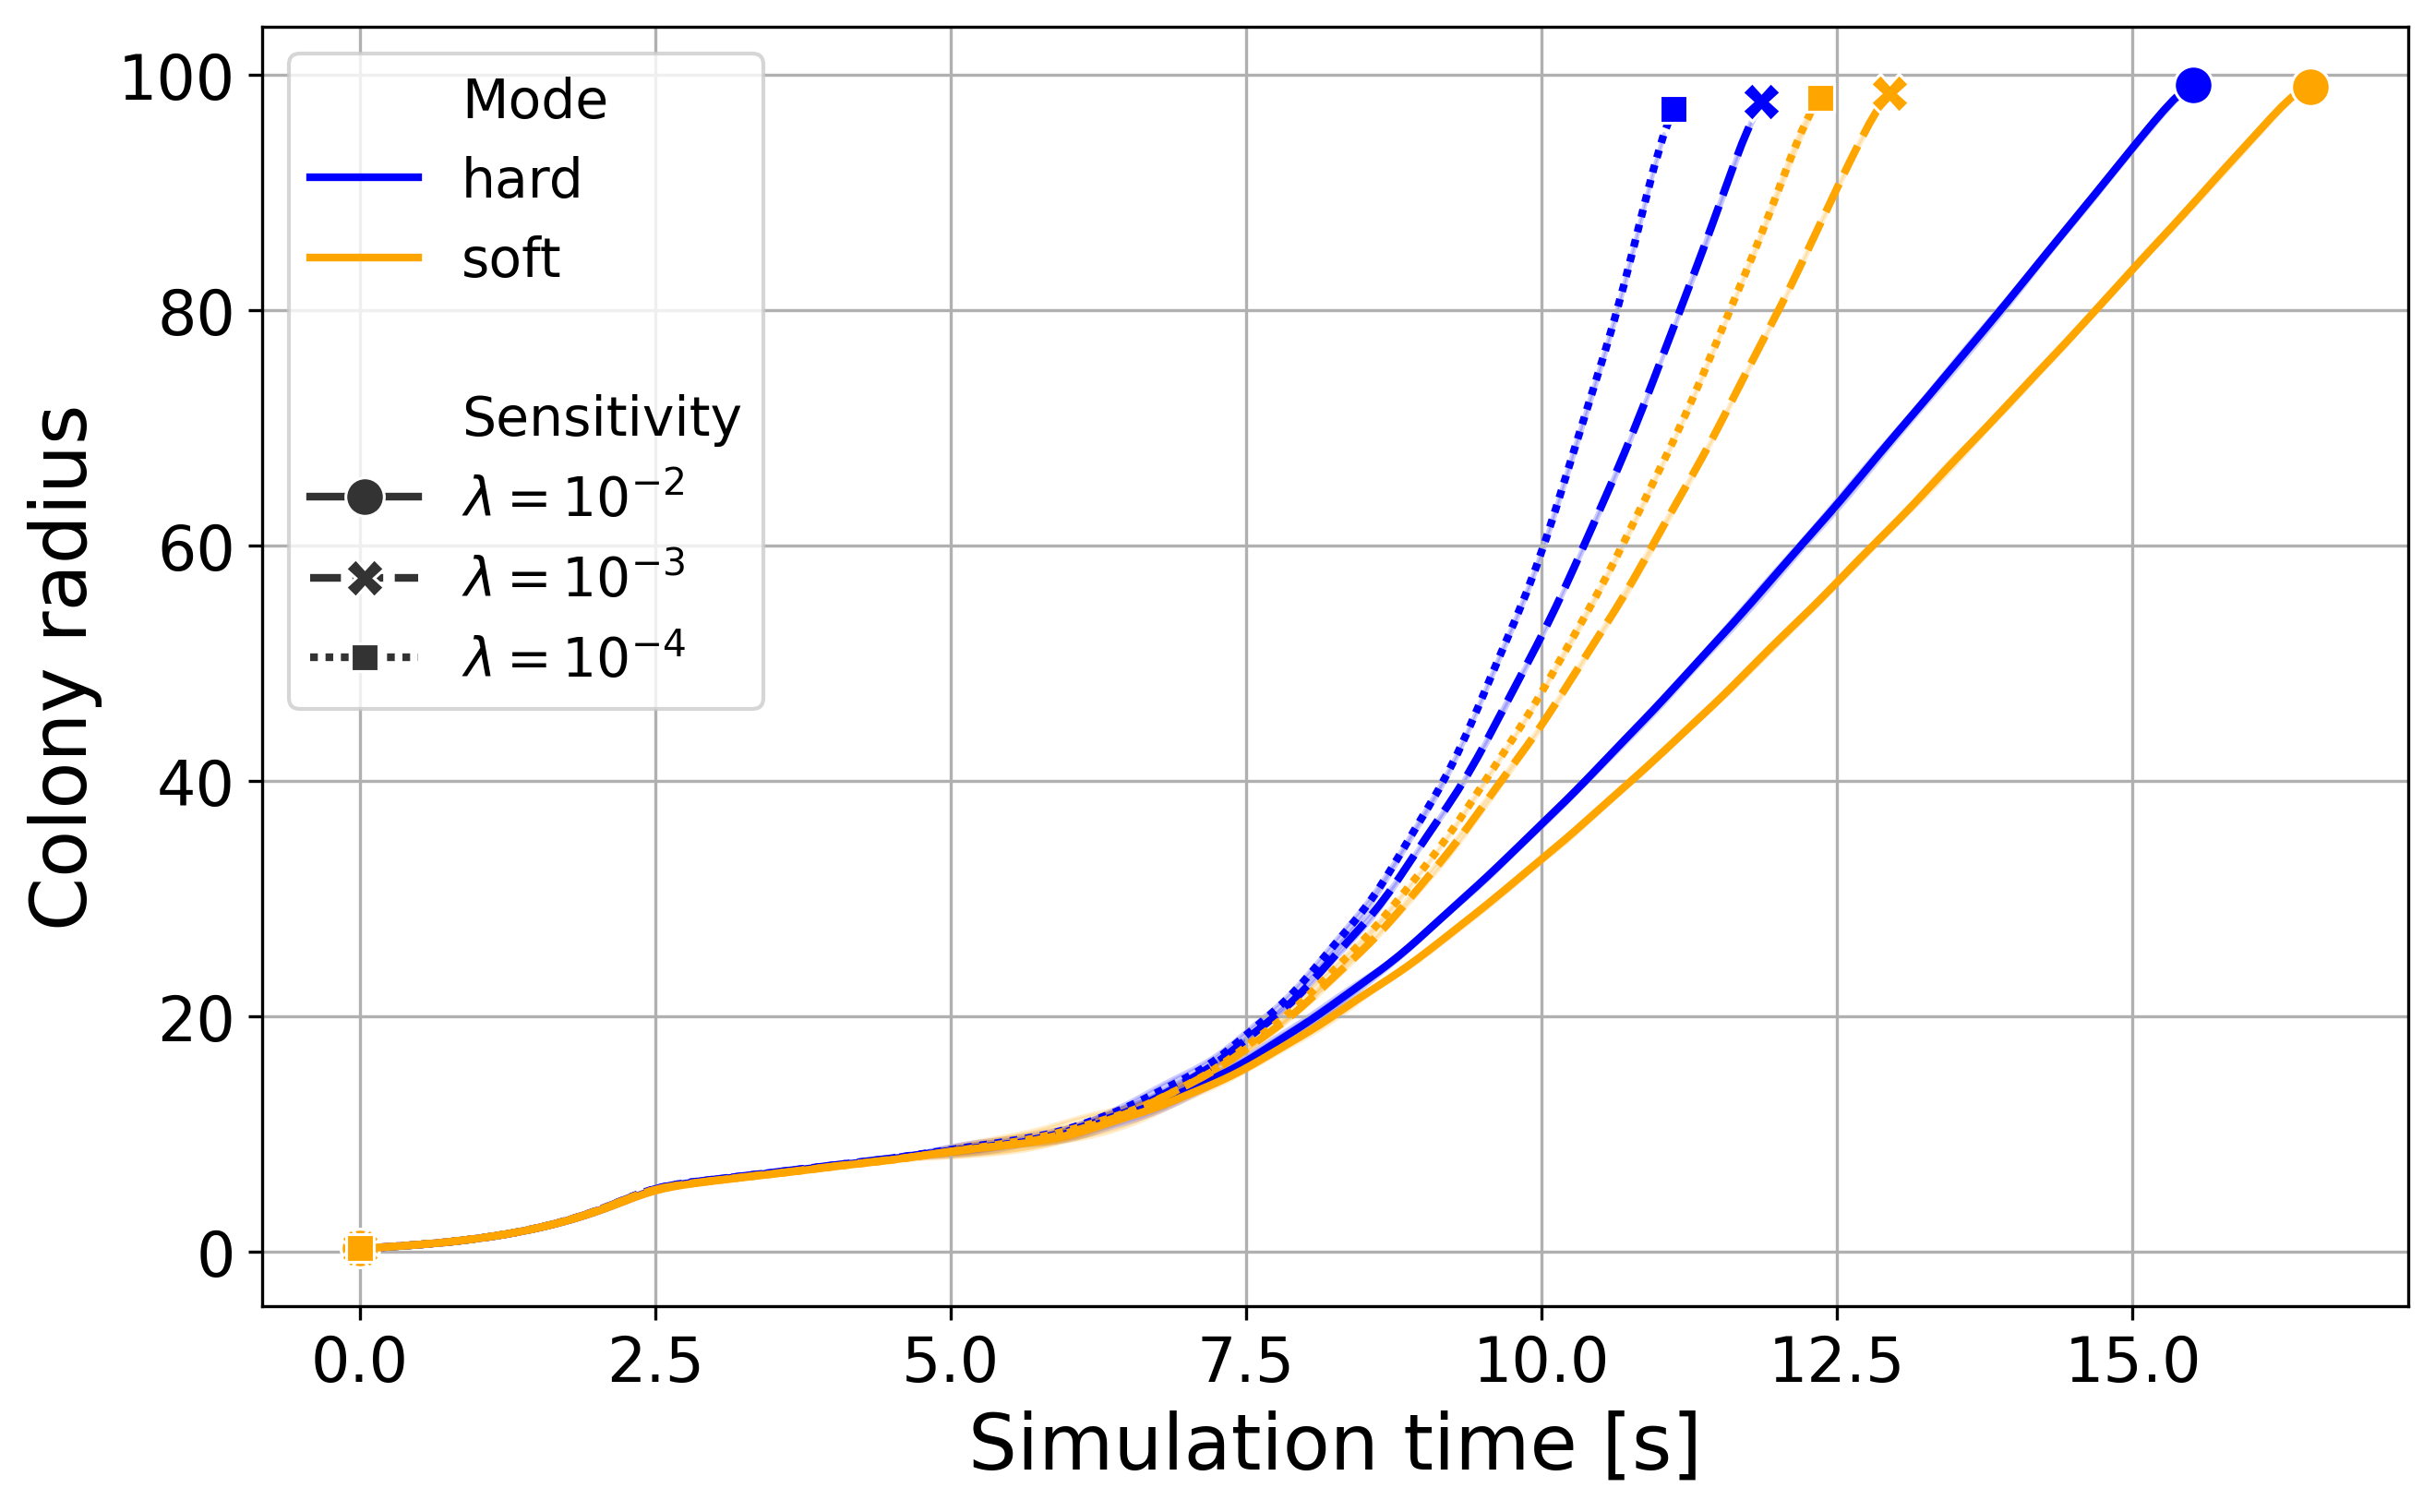
\includegraphics[width=\linewidth]{figures/comparison_plots/combined_simulation_time [s]_vs_colony_radius.png}
        \caption{Simulation time vs. colony radius. Both models exhibit similar growth dynamics, though the soft model is slightly slower due to allowable cell overlap.}
        \label{fig:sim_time_vs_colony_radius}
    \end{subfigure}

    \begin{subfigure}[b]{\linewidth}
        \centering
        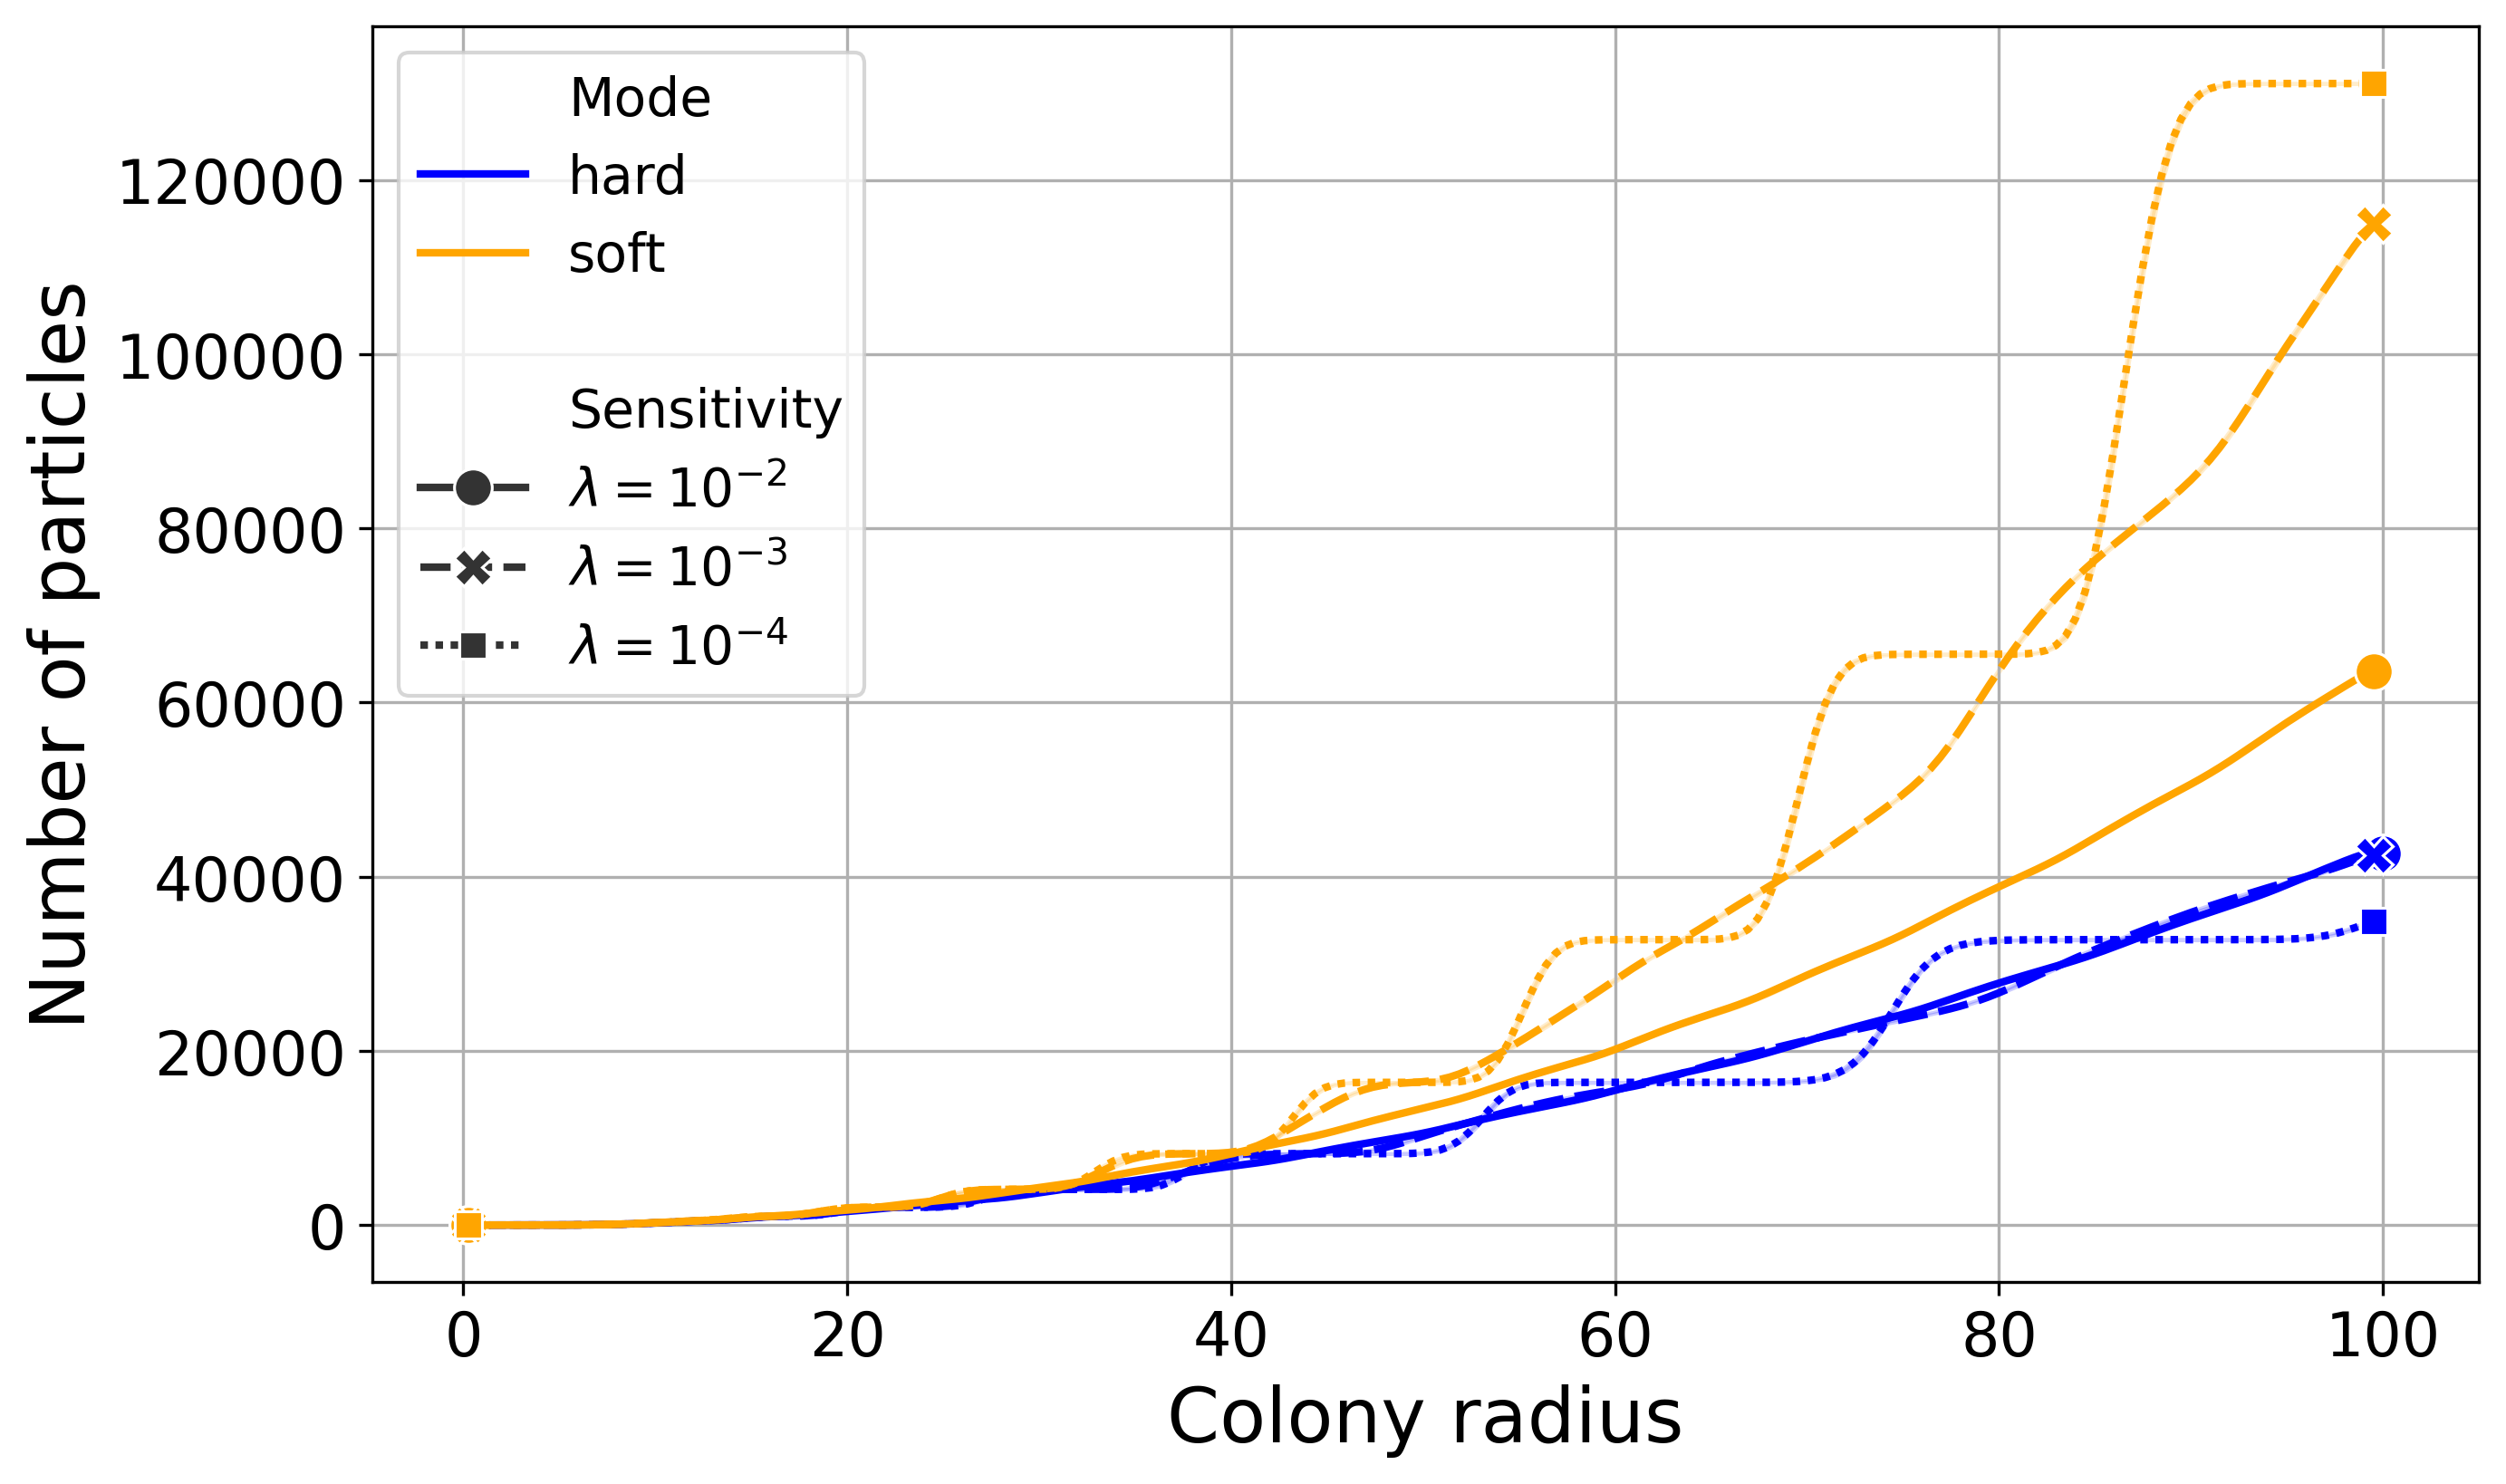
\includegraphics[width=\linewidth]{figures/comparison_plots/combined_colony_radius_vs_num_particles.png}
        \caption{Number of cells required to reach a given colony radius. The soft model requires substantially more cells, particularly at low stress-sensitivity ($\lambda = 10^{-4}$).}
        \label{fig:colony_radius_vs_num_cells}
    \end{subfigure}

    \caption{Colony growth dynamics and cell scaling comparison between hard and soft models. (a) Colony radius vs. simulation time. (b) Number of cells vs. colony radius.}
    \label{fig:comparison_combined}
\end{figure}

\subsection{Microdomain Formation}
\label{sec:microdomain_formation}

Similar to You et al.~\cite{You2018,You_2021}, we observe the formation of microdomains, defined as localized regions where cells share similar orientations. These domains emerge from mechanical interactions and growth dynamics and result in mosaic-like patterns of cell alignment within the colony.

As shown in \autoref{fig:orientation_comparison_small}, both hard and soft collision models reproduce this phenomenon for small colonies ($R \approx 50$), producing patterns that closely resemble experimental observations of real \textit{E. coli} colonies~\cite{You2018}. This agreement suggests that the essential features of microdomain formation can be captured through both collision handling approaches.

\begin{figure}[h]
    \centering
    \begin{subfigure}[b]{0.49\columnwidth}
        \centering
        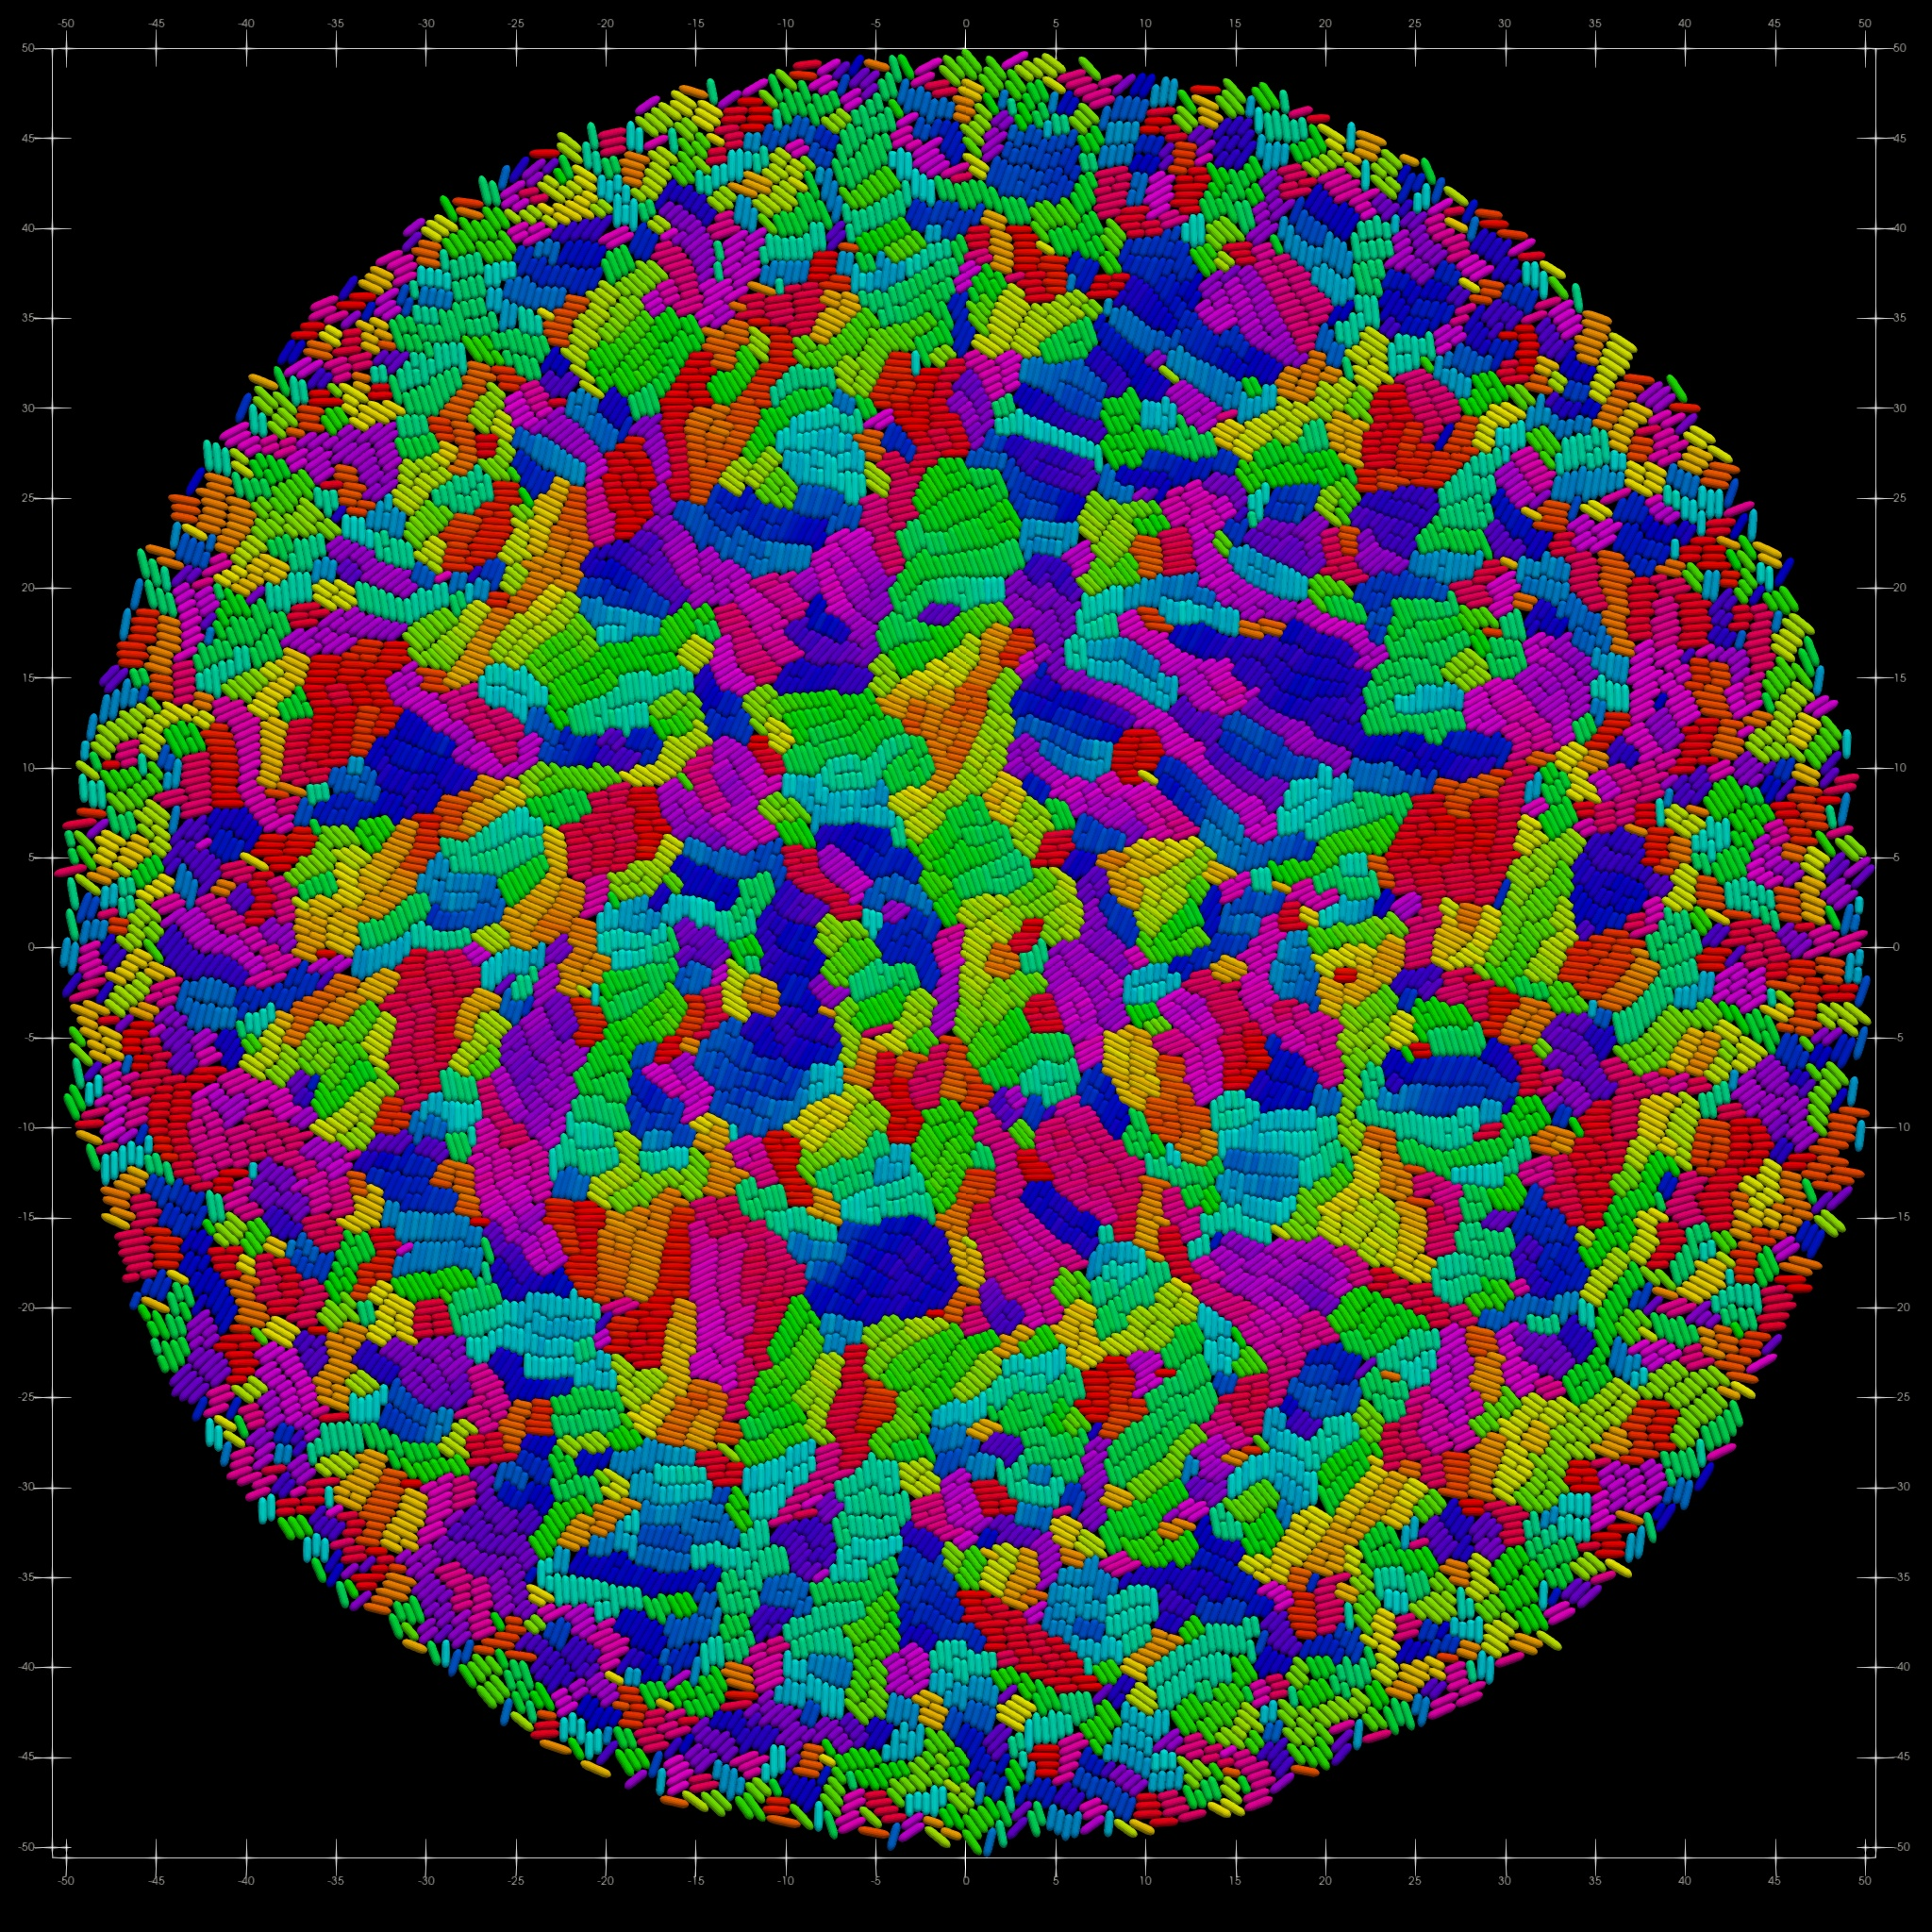
\includegraphics[width=\linewidth]{figures/orientation_comparisons/r50_soft_e-2.jpeg}
        \caption{Soft model with $\lambda = 10^{-2}$ at colony radius $R \approx 50$.}
    \end{subfigure}
    \begin{subfigure}[b]{0.49\columnwidth}
        \centering
        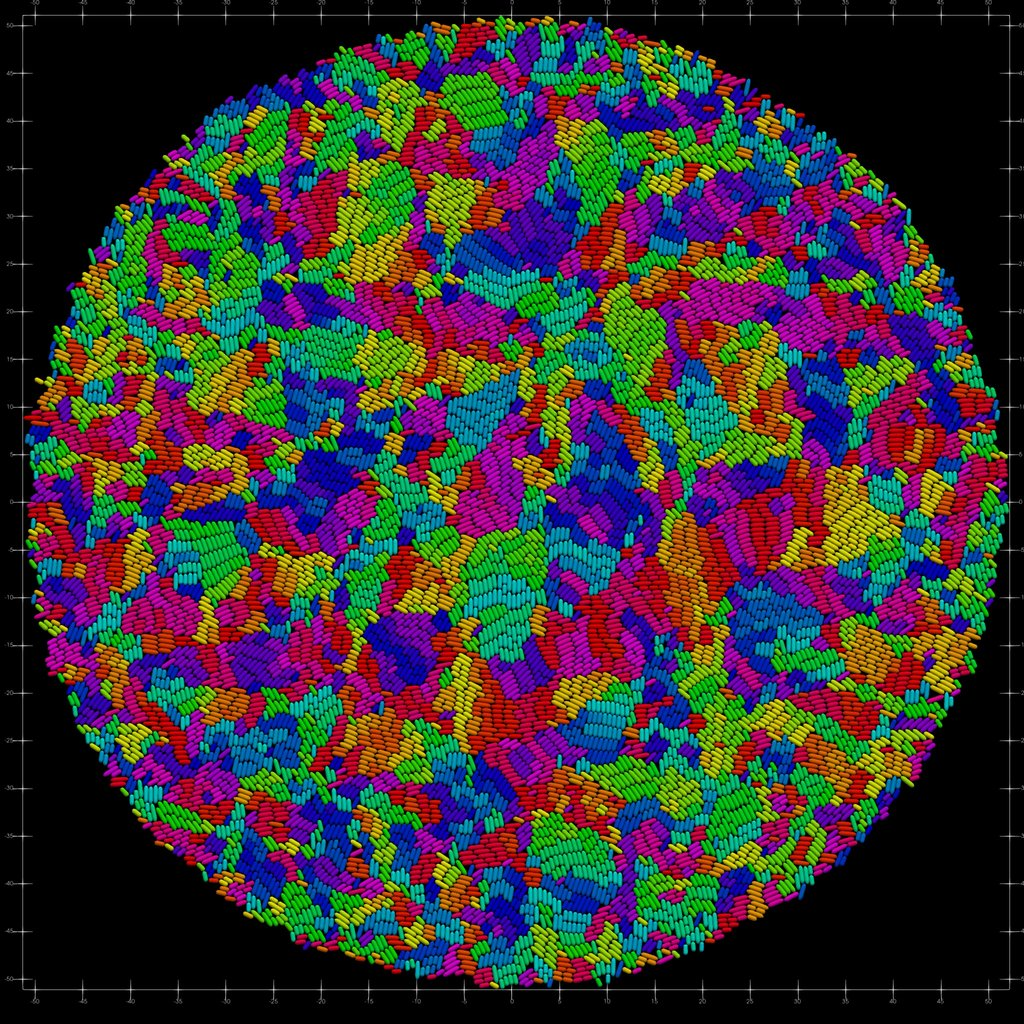
\includegraphics[width=\linewidth]{figures/orientation_comparisons/r50_hard_e-2.jpeg}
        \caption{Hard model with $\lambda = 10^{-2}$ at colony radius $R \approx 50$.}
    \end{subfigure}
    \caption{Cell orientation patterns for both models. The color indicates cell orientation angle, with similar colors representing similar angles. Both models produce comparable microdomain structures in small colonies.}
    \label{fig:orientation_comparison_small}
\end{figure}

Although the hard and soft collision models presented here are not directly comparable to You et al.~\cite{You2018}, because their study assumes constant growth rates while our models use stress-dependent growth, their findings still provide useful context. You et al. show that reduced growth rates lead to larger microdomains. In our models, stress sensitivity $\lambda$ produces a similar effect by inhibiting growth in the densely packed colony center, resulting in larger microdomains. This trend is evident in simulations of the soft model (see \autoref{fig:orientation_comparison}), where higher $\lambda$ values correspond to slower growth and larger microdomains, consistent with You et al.'s observations. The hard model, in contrast, shows no such trend. The reasons for the consistent microdomain size across $\lambda$ values could be related to the global constraint resolution, but a detailed investigation of the underlying mechanisms is beyond the scope of this comparison.

Although the hard and soft models produce similar orientation patterns in small colonies at a colony radius around $R \approx 50$ (see \autoref{fig:orientation_comparison_small}), pronounced differences emerge as colonies grow larger or $\lambda$ decreases. As shown in \autoref{fig:orientation_comparison}, the hard model maintains distinct patches of similarly-sized aligned cells across all $\lambda$ values. In contrast, the soft model produces elongated, unrealistic bundles of densely packed aligned cells that do not resemble experimentally observed microdomains.

This artifact stems directly from the soft model's higher interior growth rates, discussed in the previous chapter. Without sufficient outward stress propagation, the interior becomes unphysically dense, forcing cells into long, aligned bundles.

The effect of $\lambda$ on microdomain structure is particularly apparent in larger colonies. As shown in \autoref{fig:cluster_area_boxplot}, the hard model produces microdomains of fairly uniform size across all stress-sensitivity values, while the soft model produces larger microdomains with higher variability, as $\lambda$ decreases.

\begin{figure}[h]
    \centering
    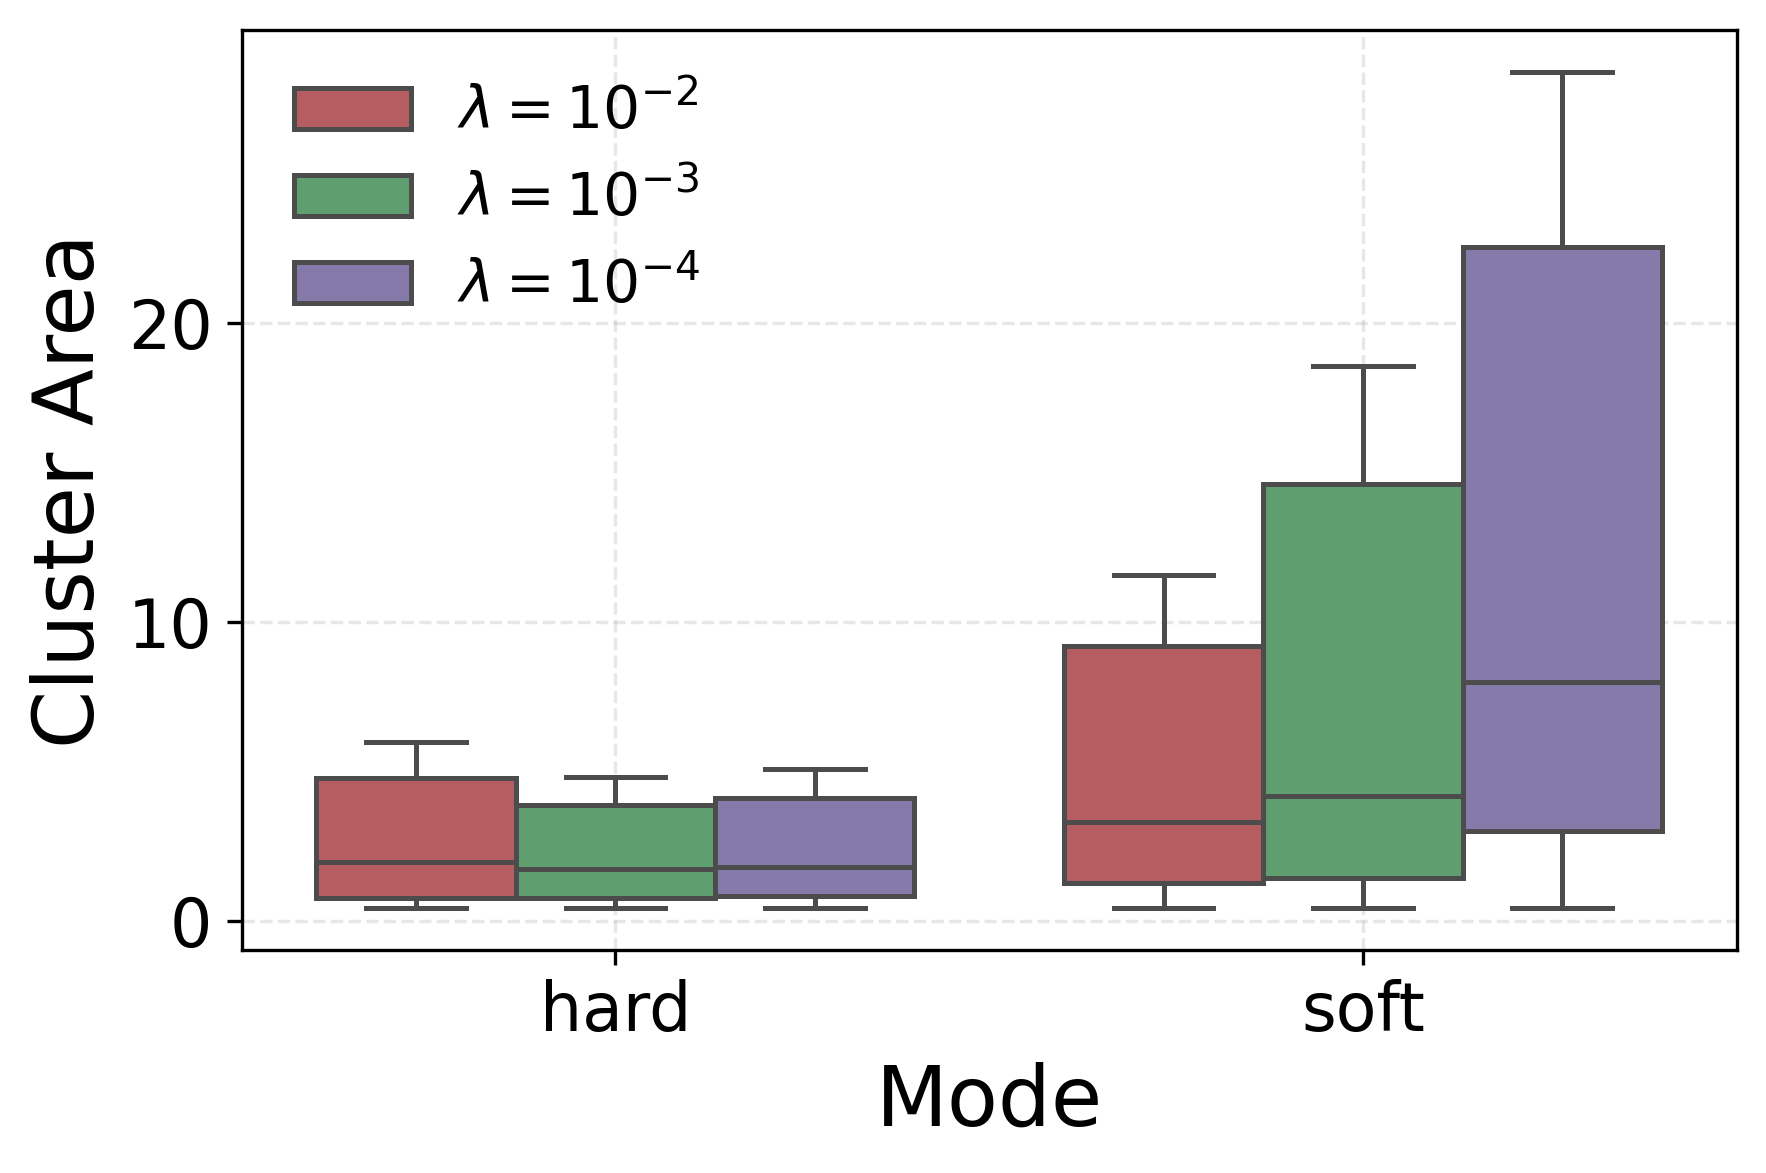
\includegraphics[width=\linewidth]{figures/comparison_plots/cluster_area_boxplot.png}
    \caption{Microdomain area distributions for large colonies ($R \approx 100$) across $\lambda$ values. The hard model produces consistent domain sizes, while the soft model shows high variability with many large clusters, especially at $\lambda = 10^{-4}$. Clusters are identified using a graph-based connected-component algorithm~\cite{You2018}, grouping neighboring cells with similar orientations (within 3\% of each other).}
    \label{fig:cluster_area_boxplot}
\end{figure}

As a consequence of bundle formation and overcrowding, the soft model is not suitable for studying microdomain formation in large colonies or in regimes of low stress sensitivity, where these effects distort the local dynamics and lead to unrealistic structural organization. In such cases, excessive overlap and artificial clustering interfere with the natural development of orientational order, preventing a faithful representation of the physical mechanisms driving microdomain formation.

Nevertheless, the soft model performs adequately for smaller colonies ($R \lesssim 50$) and at high stress-sensitivity values, where packing artifacts remain minimal and the overall orientation patterns are reasonably well captured. Within these conditions, it provides a computationally efficient and conceptually simple framework for exploring the basic principles of microdomain emergence.

For applications that require accurate characterization of microdomain properties or the exploration of weak stress-sensitivity regimes, the hard model remains the preferred choice. Future work could further examine the influence of the stress-sensitivity parameter $\lambda$ on the emergence, size, and stability of microdomains in the hard model, following an approach similar to the analyses presented by You et al.~\cite{You2018}.

\begin{figure*}[p]
    \makebox[\textwidth][c]{
        \centering

        \begin{tabular}{r M{0.36\textwidth} M{0.36\textwidth} }
             & Hard Model & Soft Model \\
            \orientationcomparisonrow{$\lambda=10^{-2}$}{-2}
            \orientationcomparisonrow{$\lambda=10^{-3}$}{-3}
            \orientationcomparisonrow{$\lambda=10^{-4}$}{-4}
        \end{tabular}
    }

    \caption{Comparison of orientation patterns at different stress sensitivities in the center of the colony. The color indicates the cell's orientation, with similar colors representing similar angles. The hard model is able to maintain visible patches of aligned cells for all stress sensitivities, whereas the soft model tends to produce long bundles of densely packed cells for low stress sensitivities. This effect is caused by a lack of separation forces, causing cells in the center of the colony to pile up.}
    \label{fig:orientation_comparison}
\end{figure*}

\newpage

\subsection{Radial Stress Distribution and Growth Rate}

Another key difference between the two modeling approaches lies in the radial stress distribution that develops within the colony (see \autoref{fig:radial_distribution_stress}). Both the hard and soft models produce qualitatively similar radially averaged stress profiles, consistent with the behavior originally reported in~\cite{Weady2024}. In both cases, the stresses are highest at the colony center and gradually decrease toward the outer edge, reflecting the buildup of mechanical compression in the densely packed interior. These profiles approximately follow the derived analytical expression $\tilde{\sigma}(r) \approx \frac{2}{\lambda} \ln\left(\frac{1}{8 c} - c\lambda r^2 \right)$~\cite{Weady2024SM}, which predicts a logarithmic dependence on the colony radius.

Although the overall shape of the profiles is comparable, the magnitude of the predicted stresses differs substantially between the two models. Quantitatively, the hard model produces stress values that are up to two times higher than the analytical prediction, whereas the soft model yields stresses that are only about half the analytical value. This variation in stress magnitude is significant and likely plays a central role in explaining the discrepancies in growth dynamics and microdomain organization discussed in \autoref{sec:colony_growth_dynamics} and \autoref{sec:microdomain_formation}.

\begin{figure*}[b]
    \centering
    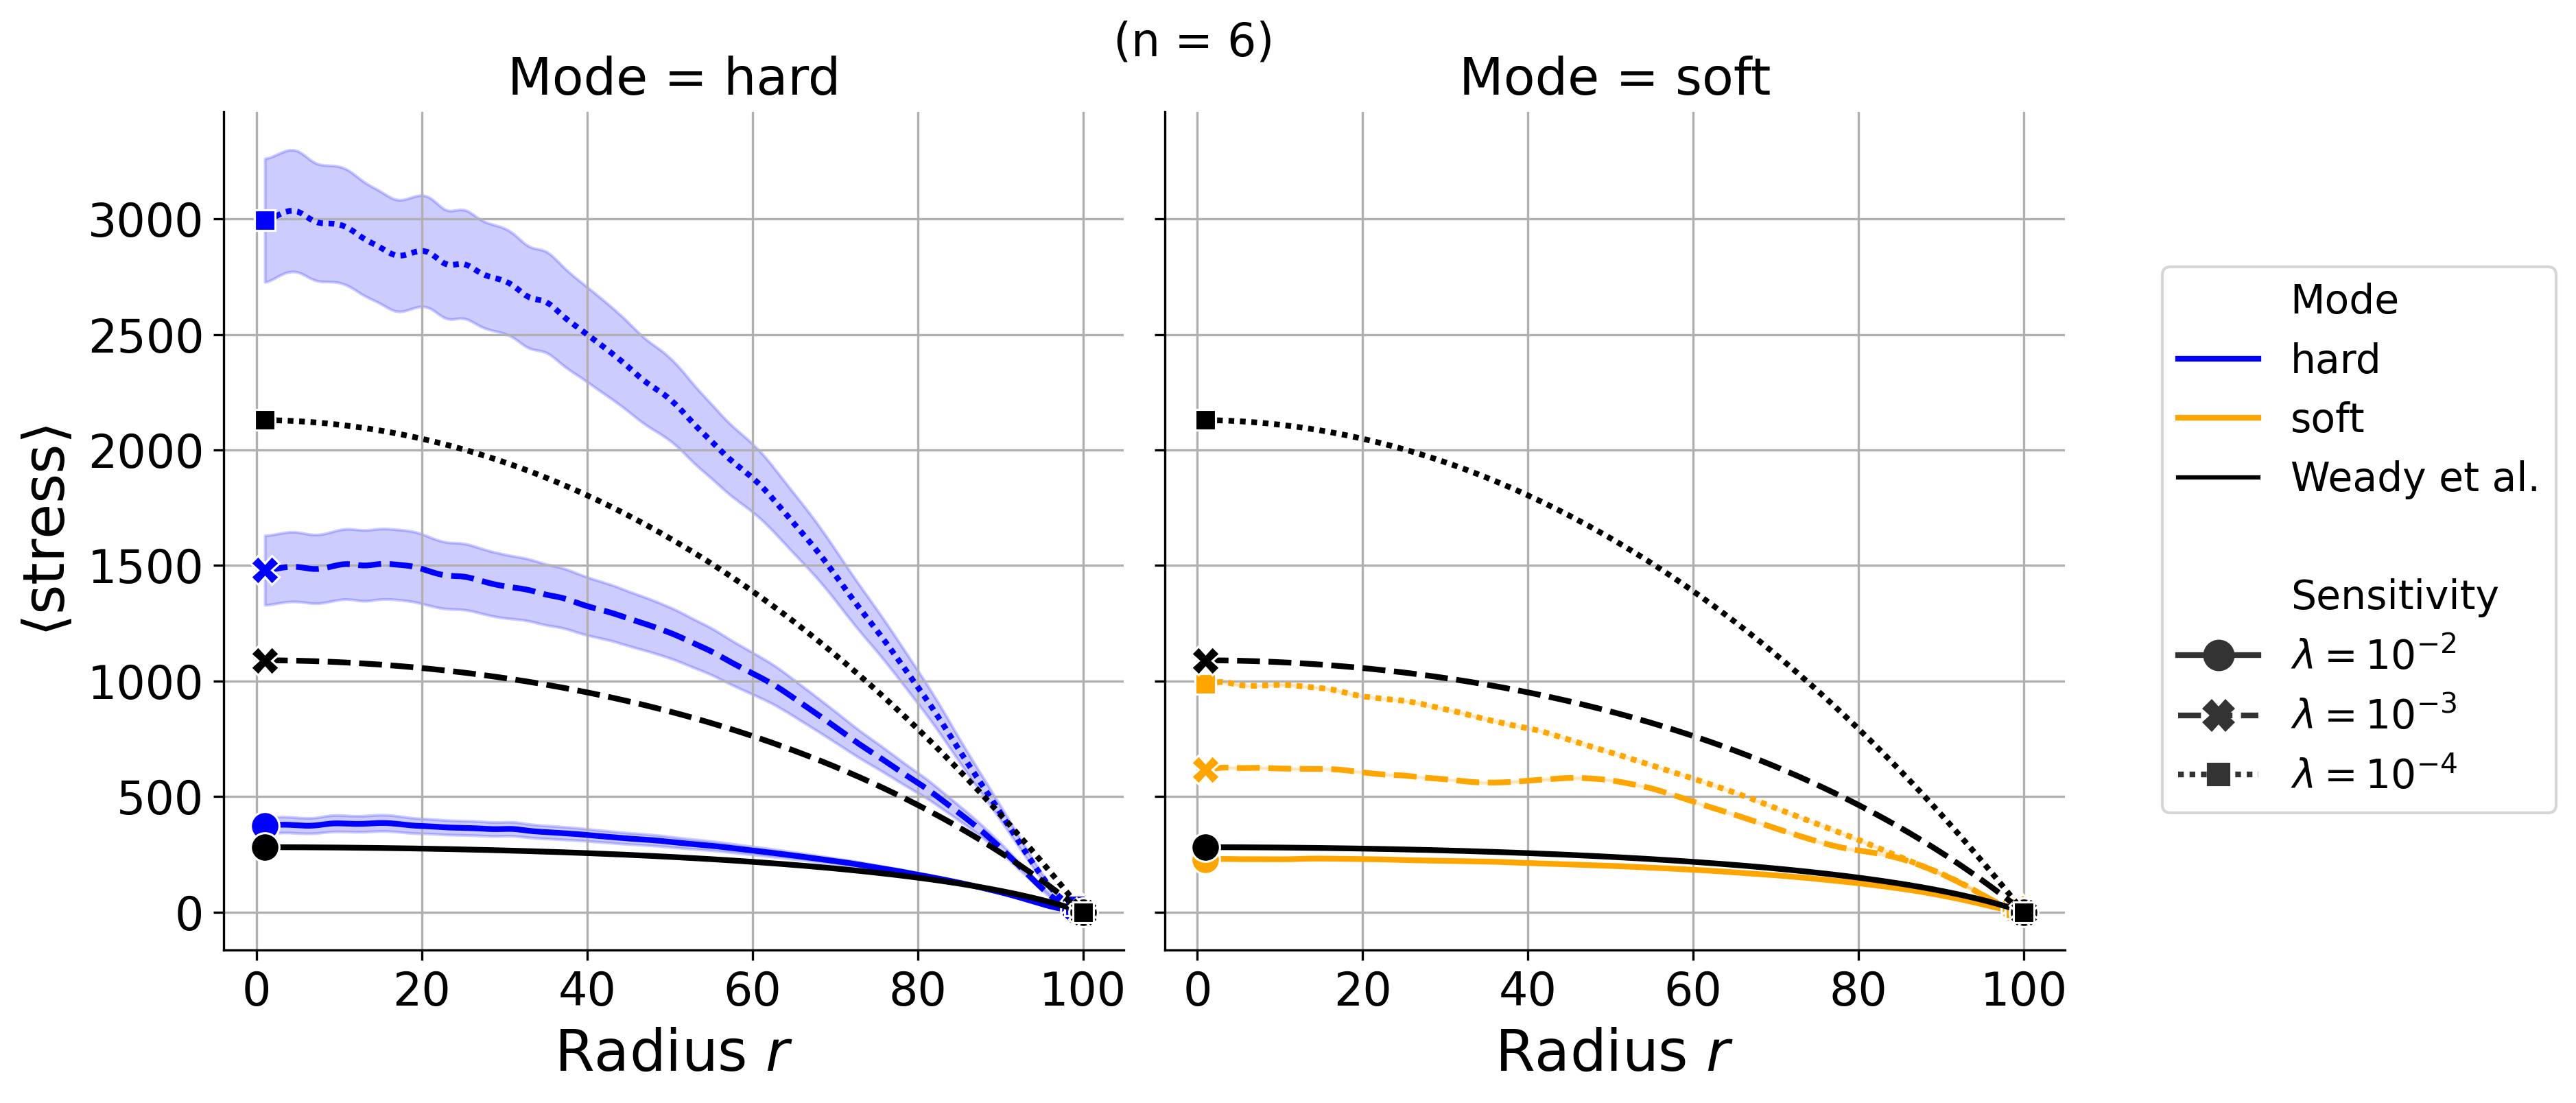
\includegraphics[width=\linewidth]{figures/comparison_plots/combined_stress_shared.png}
    \caption{Radial stress profiles for both models across different $\lambda$ values. Both models exhibit similar qualitative trends, with stresses peaking at the colony center and decreasing toward the edge. However, the hard model consistently produces higher stress magnitudes compared to the soft model. The dashed lines represent the analytical prediction from~\cite{Weady2024SM}.}
    \label{fig:radial_distribution_stress}
\end{figure*}

The consistently elevated stresses observed in the hard model are also noted by Weady et al.~\cite{Weady2024} and are likely a consequence of the discrete cell-based representation not fully satisfying the continuum assumptions used in the analytical derivation.

In contrast, the soft model produces lower stresses because it lacks a global force propagation mechanism: stress is transmitted only through local pairwise repulsive interactions, which are insufficient to communicate mechanical load effectively across the entire colony. Consequently, stresses in the colony interior remain low, and central cells experience weaker mechanical inhibition. These cells therefore continue to grow and divide, eventually leading to the overcrowding and distorted microdomain patterns.

As shown in \autoref{fig:radial_distribution_growth_rate}, the differences in stress transmission directly manifest in the radial growth rate profiles. Cells in the soft model exhibit substantially higher growth rates than those in the hard model across most of the colony interior, particularly at low stress-sensitivity values. At higher stress-sensitivity ($\lambda = 10^{-2}$), growth becomes strongly suppressed in the colony interior for both models, and only cells located near the periphery remain actively dividing. The resulting shift from interior-driven to edge-driven proliferation is also clearly visible in \autoref{fig:sim_time_vs_colony_radius} and mirrors a well-documented behavior in real microbial systems, such as in bacterial and yeast colonies, including \textit{E. coli} and \textit{Saccharomyces cerevisiae}, where mechanical feedback and nutrient depletion restrict active expansion to the growing front~\cite{Warren2019,Hallatschek2007,Giometto2018}.

\begin{figure}[H]
    \centering
    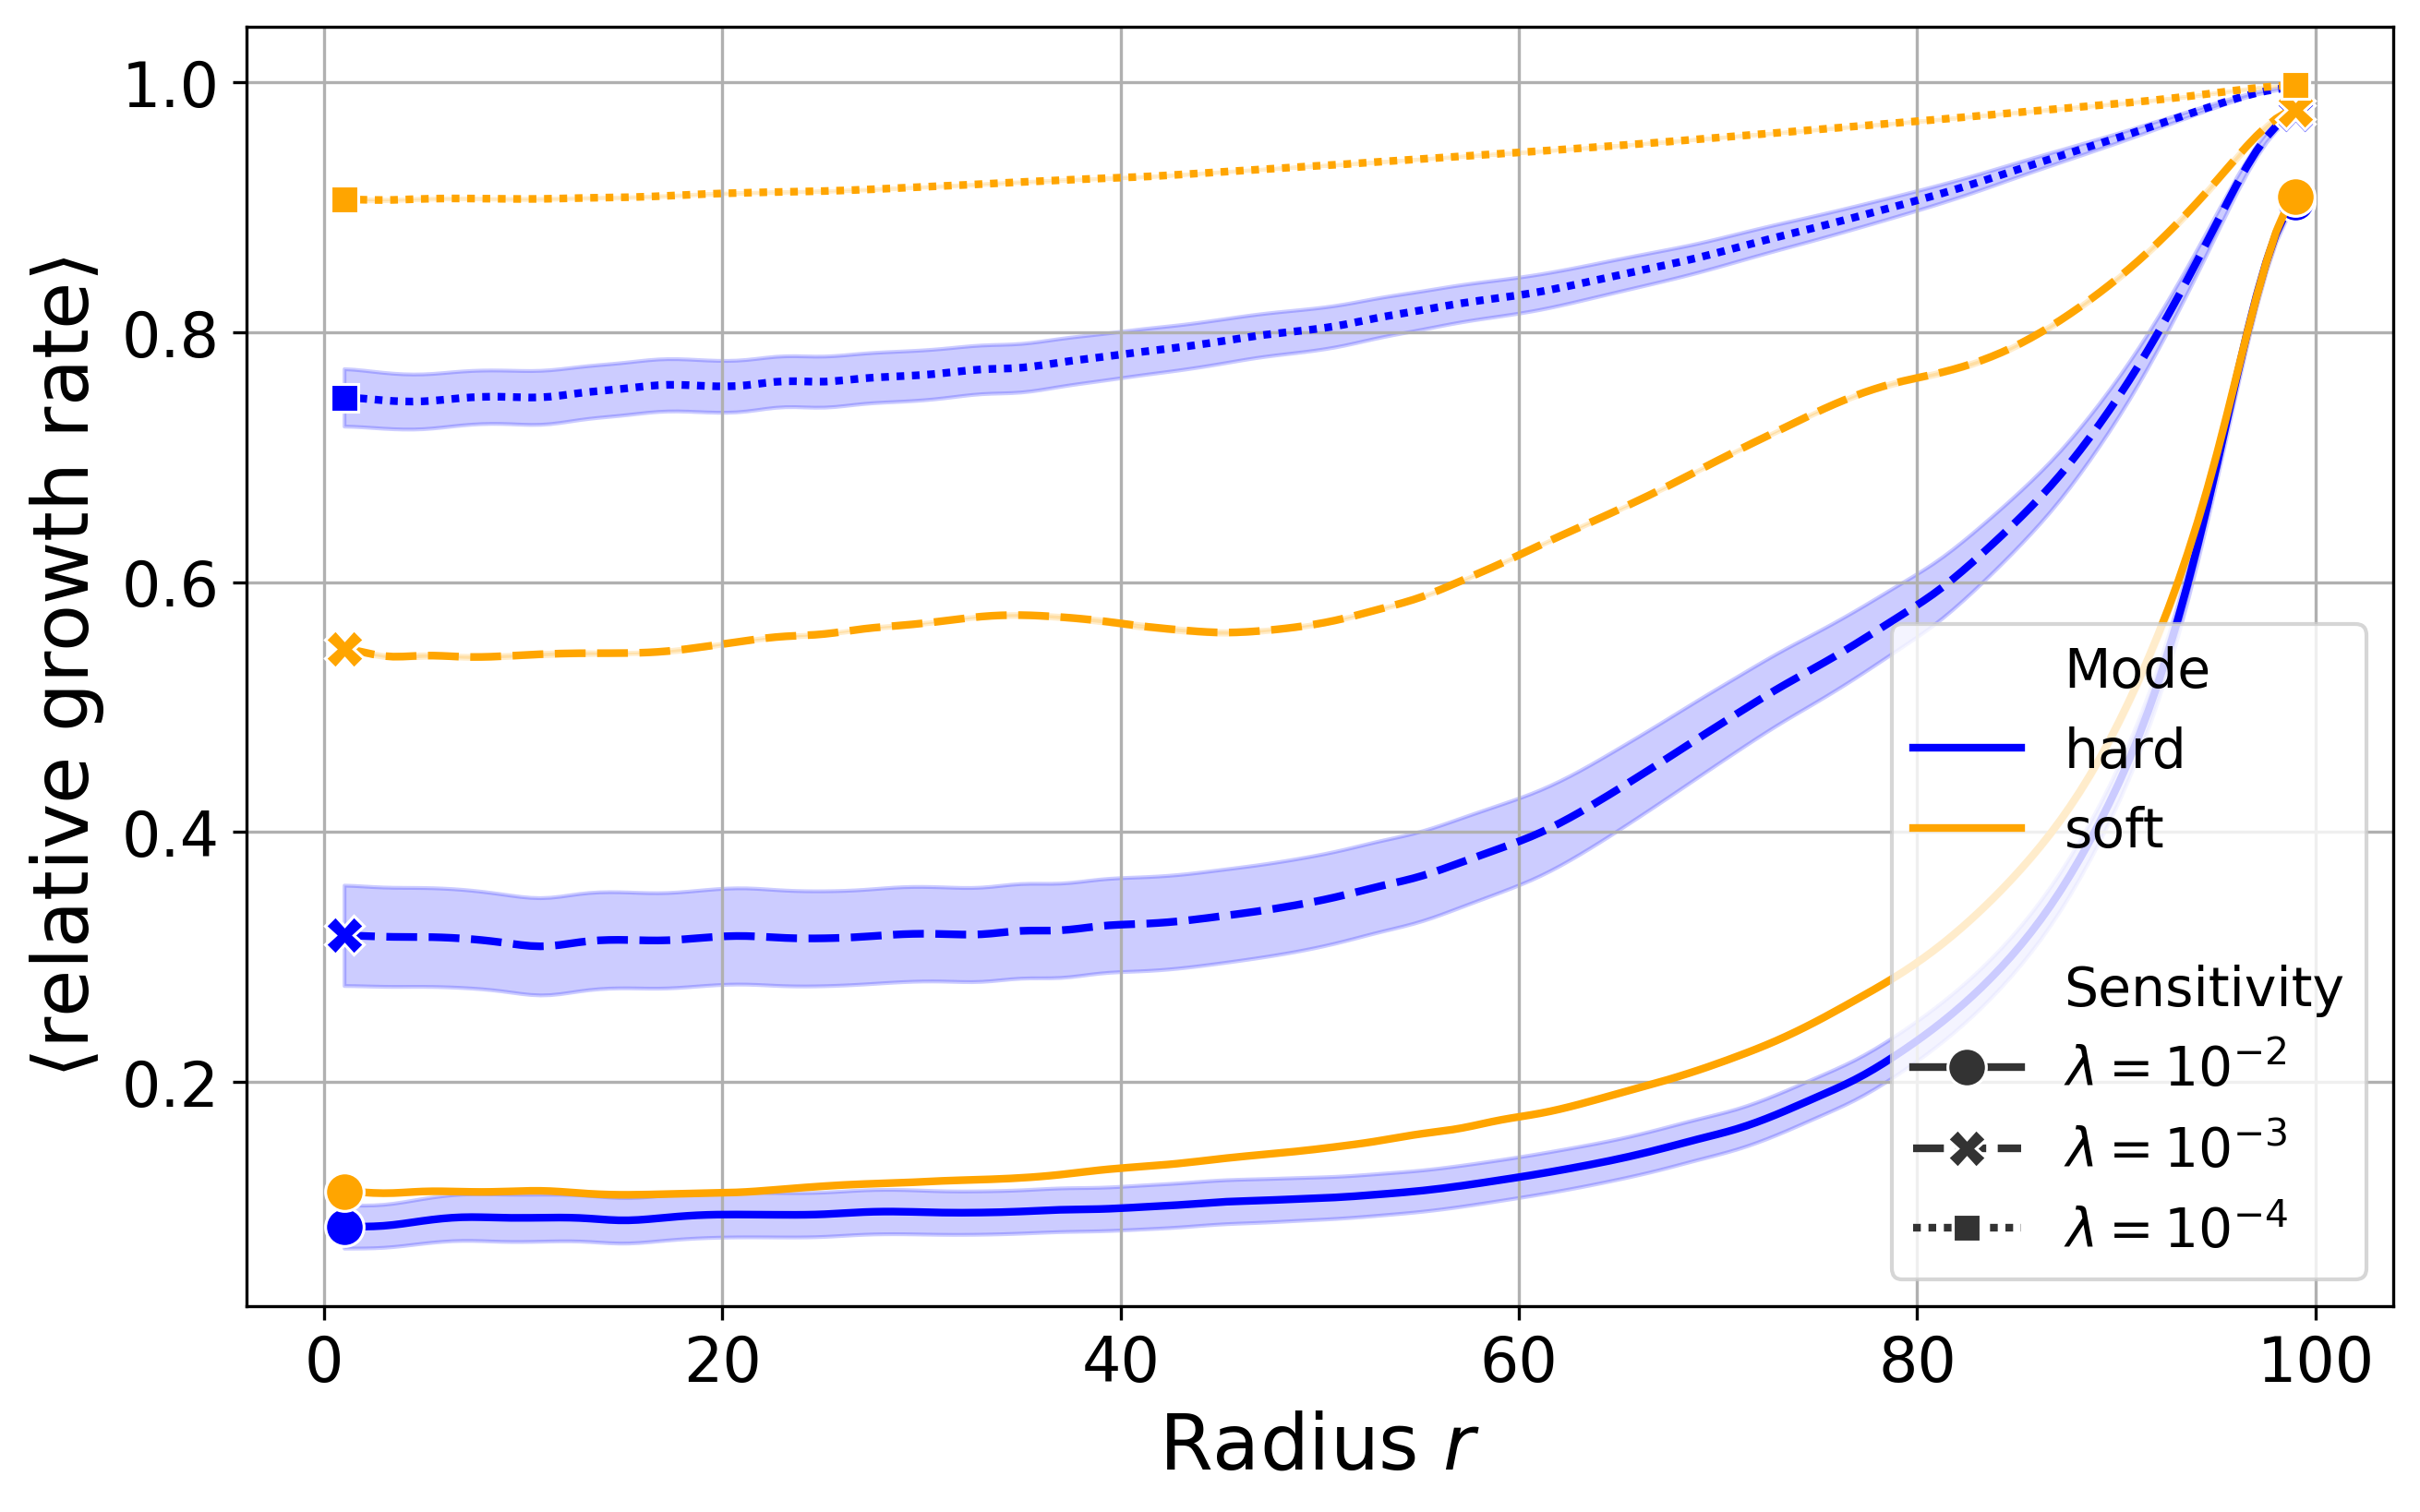
\includegraphics[width=\linewidth]{figures/comparison_plots/combined_radial_impedance.png}
    \caption{Radial relative growth rate profiles ($e^{-\lambda \sigma}$) for both models. Cells in the soft model grow significantly faster than those in the hard model across most of the colony, particularly at low stress-sensitivity ($\lambda = 10^{-3}$ and $\lambda = 10^{-4}$). At high stress-sensitivity ($\lambda = 10^{-2}$), growth is strongly suppressed in the interior of both models, with only cells at the colony edge actively dividing.}
    \label{fig:radial_distribution_growth_rate}
\end{figure}

\section{Computational Performance}
\label{sec:performance_analysis}

As shown in the previous section, both the hard and soft collision models reproduce experimentally observed macroscopic patterns but differ in computational performance. This section compares their computational efficiency in detail. Benchmarks are conducted on the \texttt{CoolMUC-4}\footnote{\texttt{CoolMUC-4} is part of the Linux Cluster at the Leibniz Supercomputing Centre (LRZ). It consists of 106 compute nodes equipped with \textit{Intel Xeon Platinum 8480+ (Sapphire Rapids)} CPUs, each providing 112 cores. For details, see \url{https://doku.lrz.de/coolmuc-4-1082337877.html}.} HPC cluster.

The simulations employ a domain decomposition strategy that divides the computational domain into equally sized rectangular subdomains, each assigned to a single MPI rank. Due to the initially localized nature of cell colonies, a significant load imbalance exists at the beginning of the simulation but gradually decreases as the colony expands and occupies a larger portion of the domain.

\subsection{Critical Timestep}
\autoref{fig:simulation_time_vs_dt} shows the critical timestep $\Delta t$ determined by \autoref{alg:adaptive_dt} for both models during a simulation. The hard model stabilizes around $\Delta t_{\text{hard}} \approx 3 \cdot 10^{-4}$ h, while the soft model steadily decreases to $\Delta t_{\text{soft}} \approx 10^{-5}$ h. The ratio $\Delta t_{\text{hard}}/\Delta t_{\text{soft}} \approx 30$ indicates the hard model can take roughly 30 times larger steps than the soft model in dense colonies, requiring significantly fewer steps to simulate equivalent physical time. Notably, for the hard model with $\lambda = 10^{-2}$, the critical timestep increases over time, as cell growth in the interior slows down (see \autoref{fig:radial_distribution_growth_rate}) and the overall median velocity $u_m$ decreases.

Adaptive time stepping ensures stability and efficiency throughout the simulation by adjusting the temporal resolution to the system's current dynamics. A fixed timestep cannot achieve this balance: small steps are wasteful during early growth when interactions are sparse, while large steps cause numerical instability and potential failure in dense colonies. Since no single timestep is optimal for all stages, adaptivity is essential for robust long-term simulations.

\begin{figure}[H]
    \centering
    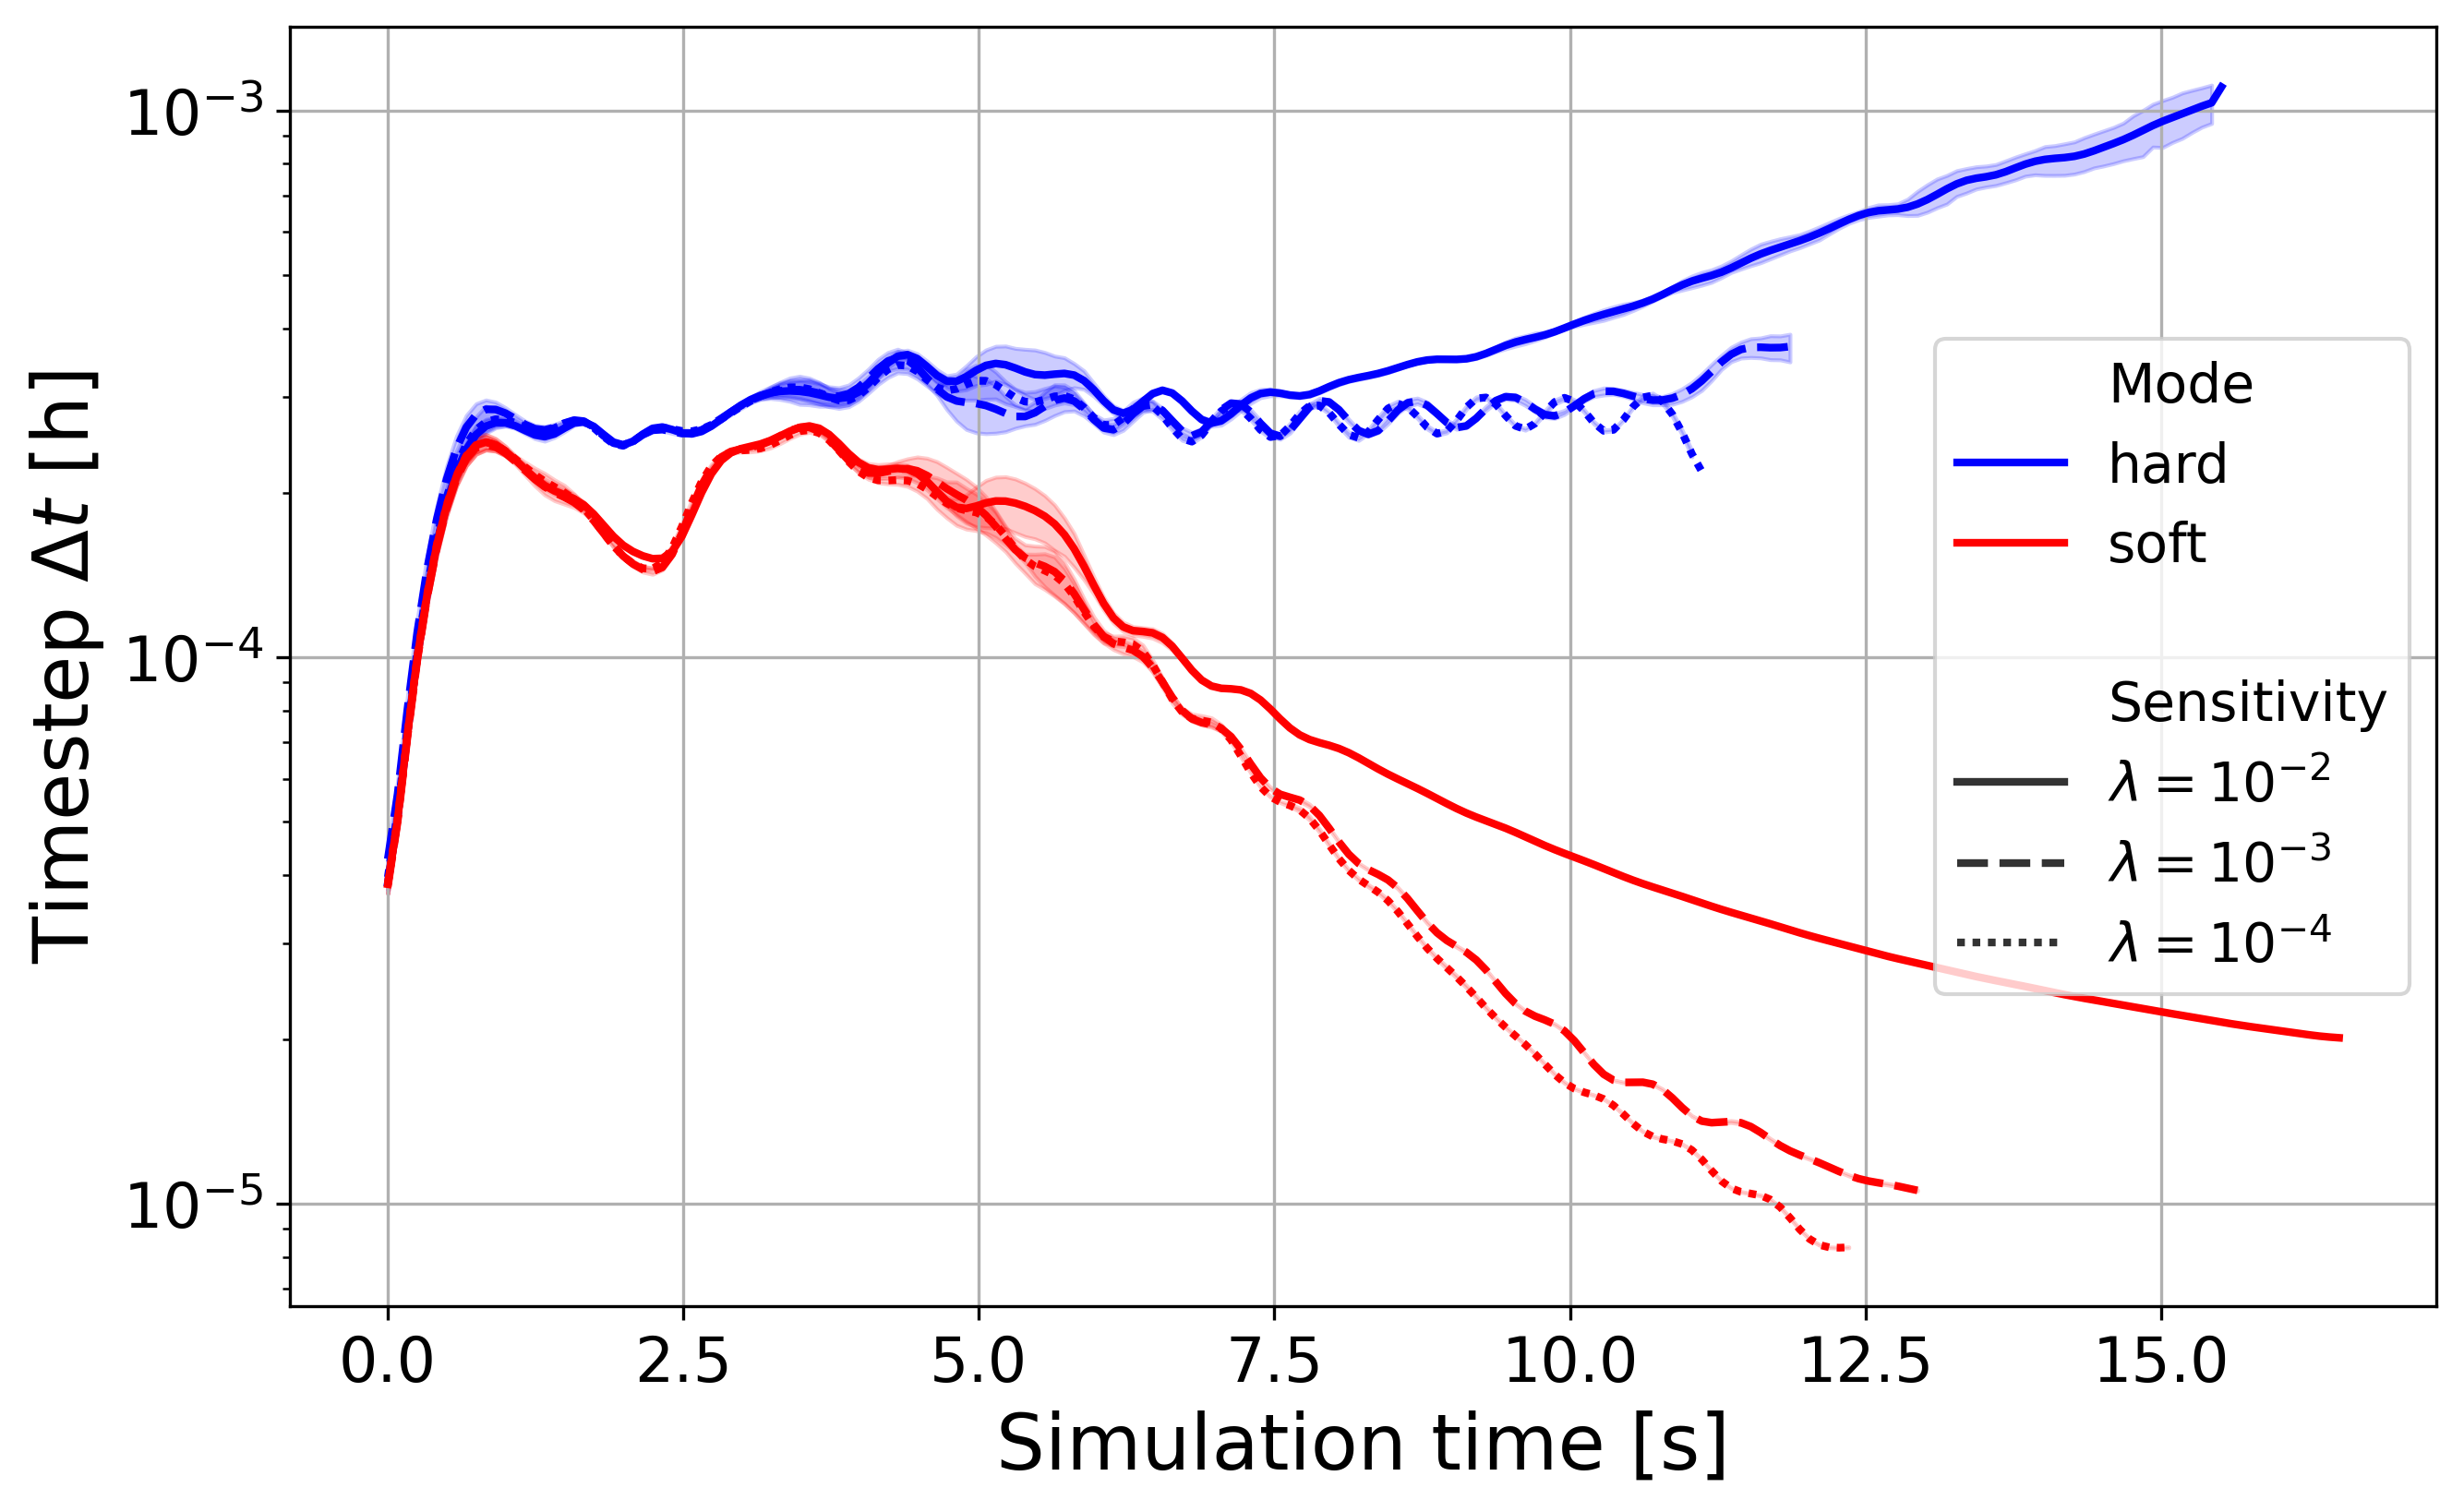
\includegraphics[width=\linewidth]{figures/comparison_plots/combined_simulation_time [s]_vs_dt.png}
    \caption{Adaptive timestep $\Delta t$ over simulation time for both collision models. The hard model stabilizes around $\Delta t_{\text{hard}} \approx 3 \cdot 10^{-4}$ h, while the soft model tends to $\Delta t_{\text{soft}} \approx 1 \cdot 10^{-5}$ h.}
    \label{fig:simulation_time_vs_dt}
\end{figure}

\subsection{Strong Scaling}
\label{sec:strong_scaling}

To assess parallel performance, we analyze runtime and speedup as functions of CPU core count. In the strong-scaling tests, colonies grow from a single cell to a radius of 100, allowing us to measure how efficiently each model utilizes increasing computational resources.

At low core counts, the hard model outperforms the soft model by approximately 20\% (see \autoref{fig:runtime_hard_soft}), likely because it can advance with larger timesteps. As the number of cores increases, the runtimes of both models converge. The speedup data in \autoref{fig:speedup_hard_soft} indicate that the soft model scales efficiently up to a 20$\times$ speedup at 112 ranks, while the hard model exhibits reduced scaling efficiency beyond 20 ranks.

The soft model's weaker performance at low core counts partly stems from its higher packing density, which requires more cells to reach the same colony radius (see \autoref{fig:colony_radius_vs_num_cells}), and from its smaller stable timesteps (see \autoref{fig:simulation_time_vs_dt}). For larger simulations ($R > 100$), this trend reverses, and the soft model becomes increasingly advantageous (see \autoref{sec:maximum_colony_size}).

\begin{figure}[H]
    \centering
    \begin{subfigure}[b]{1\linewidth}
        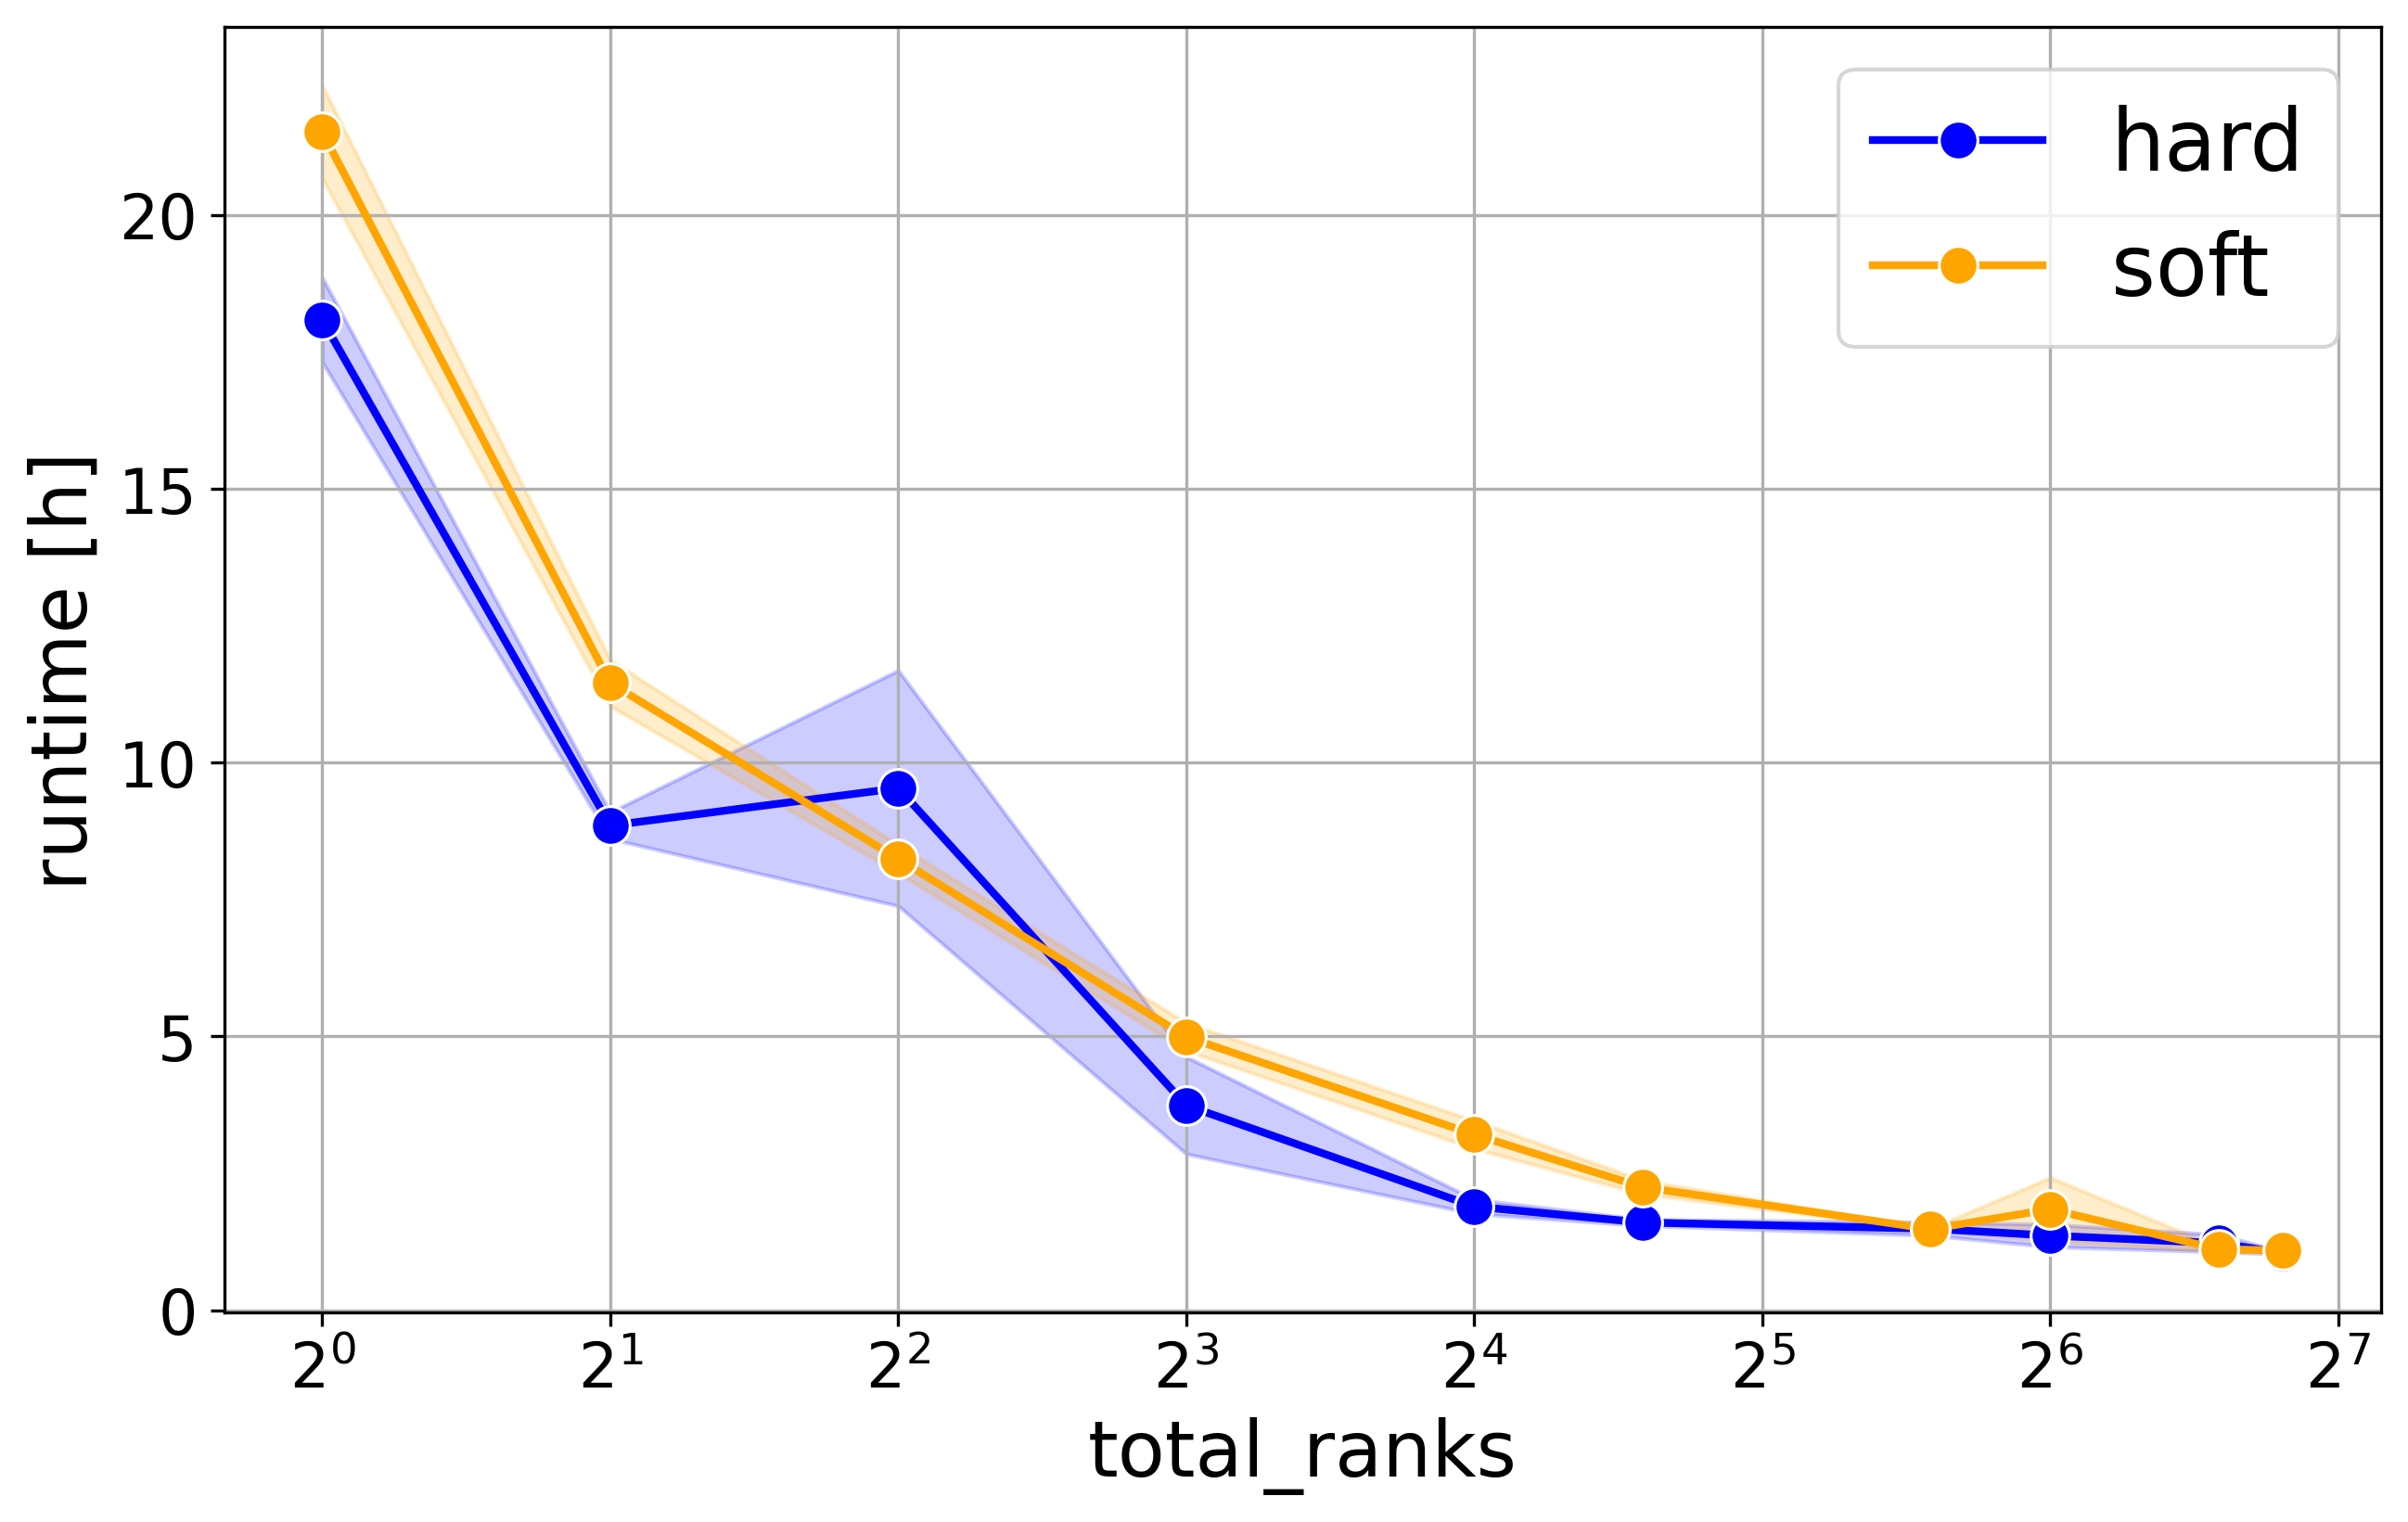
\includegraphics[width=\linewidth]{figures/runtimes/strong_scaling_runtime_hard_soft.png}
        \caption{Runtime to reach a colony radius of 100 versus CPU cores. The hard model is slightly faster at low core counts, but both models converge at higher core counts.}
        \label{fig:runtime_hard_soft}
    \end{subfigure}

    \begin{subfigure}[b]{1\linewidth}
        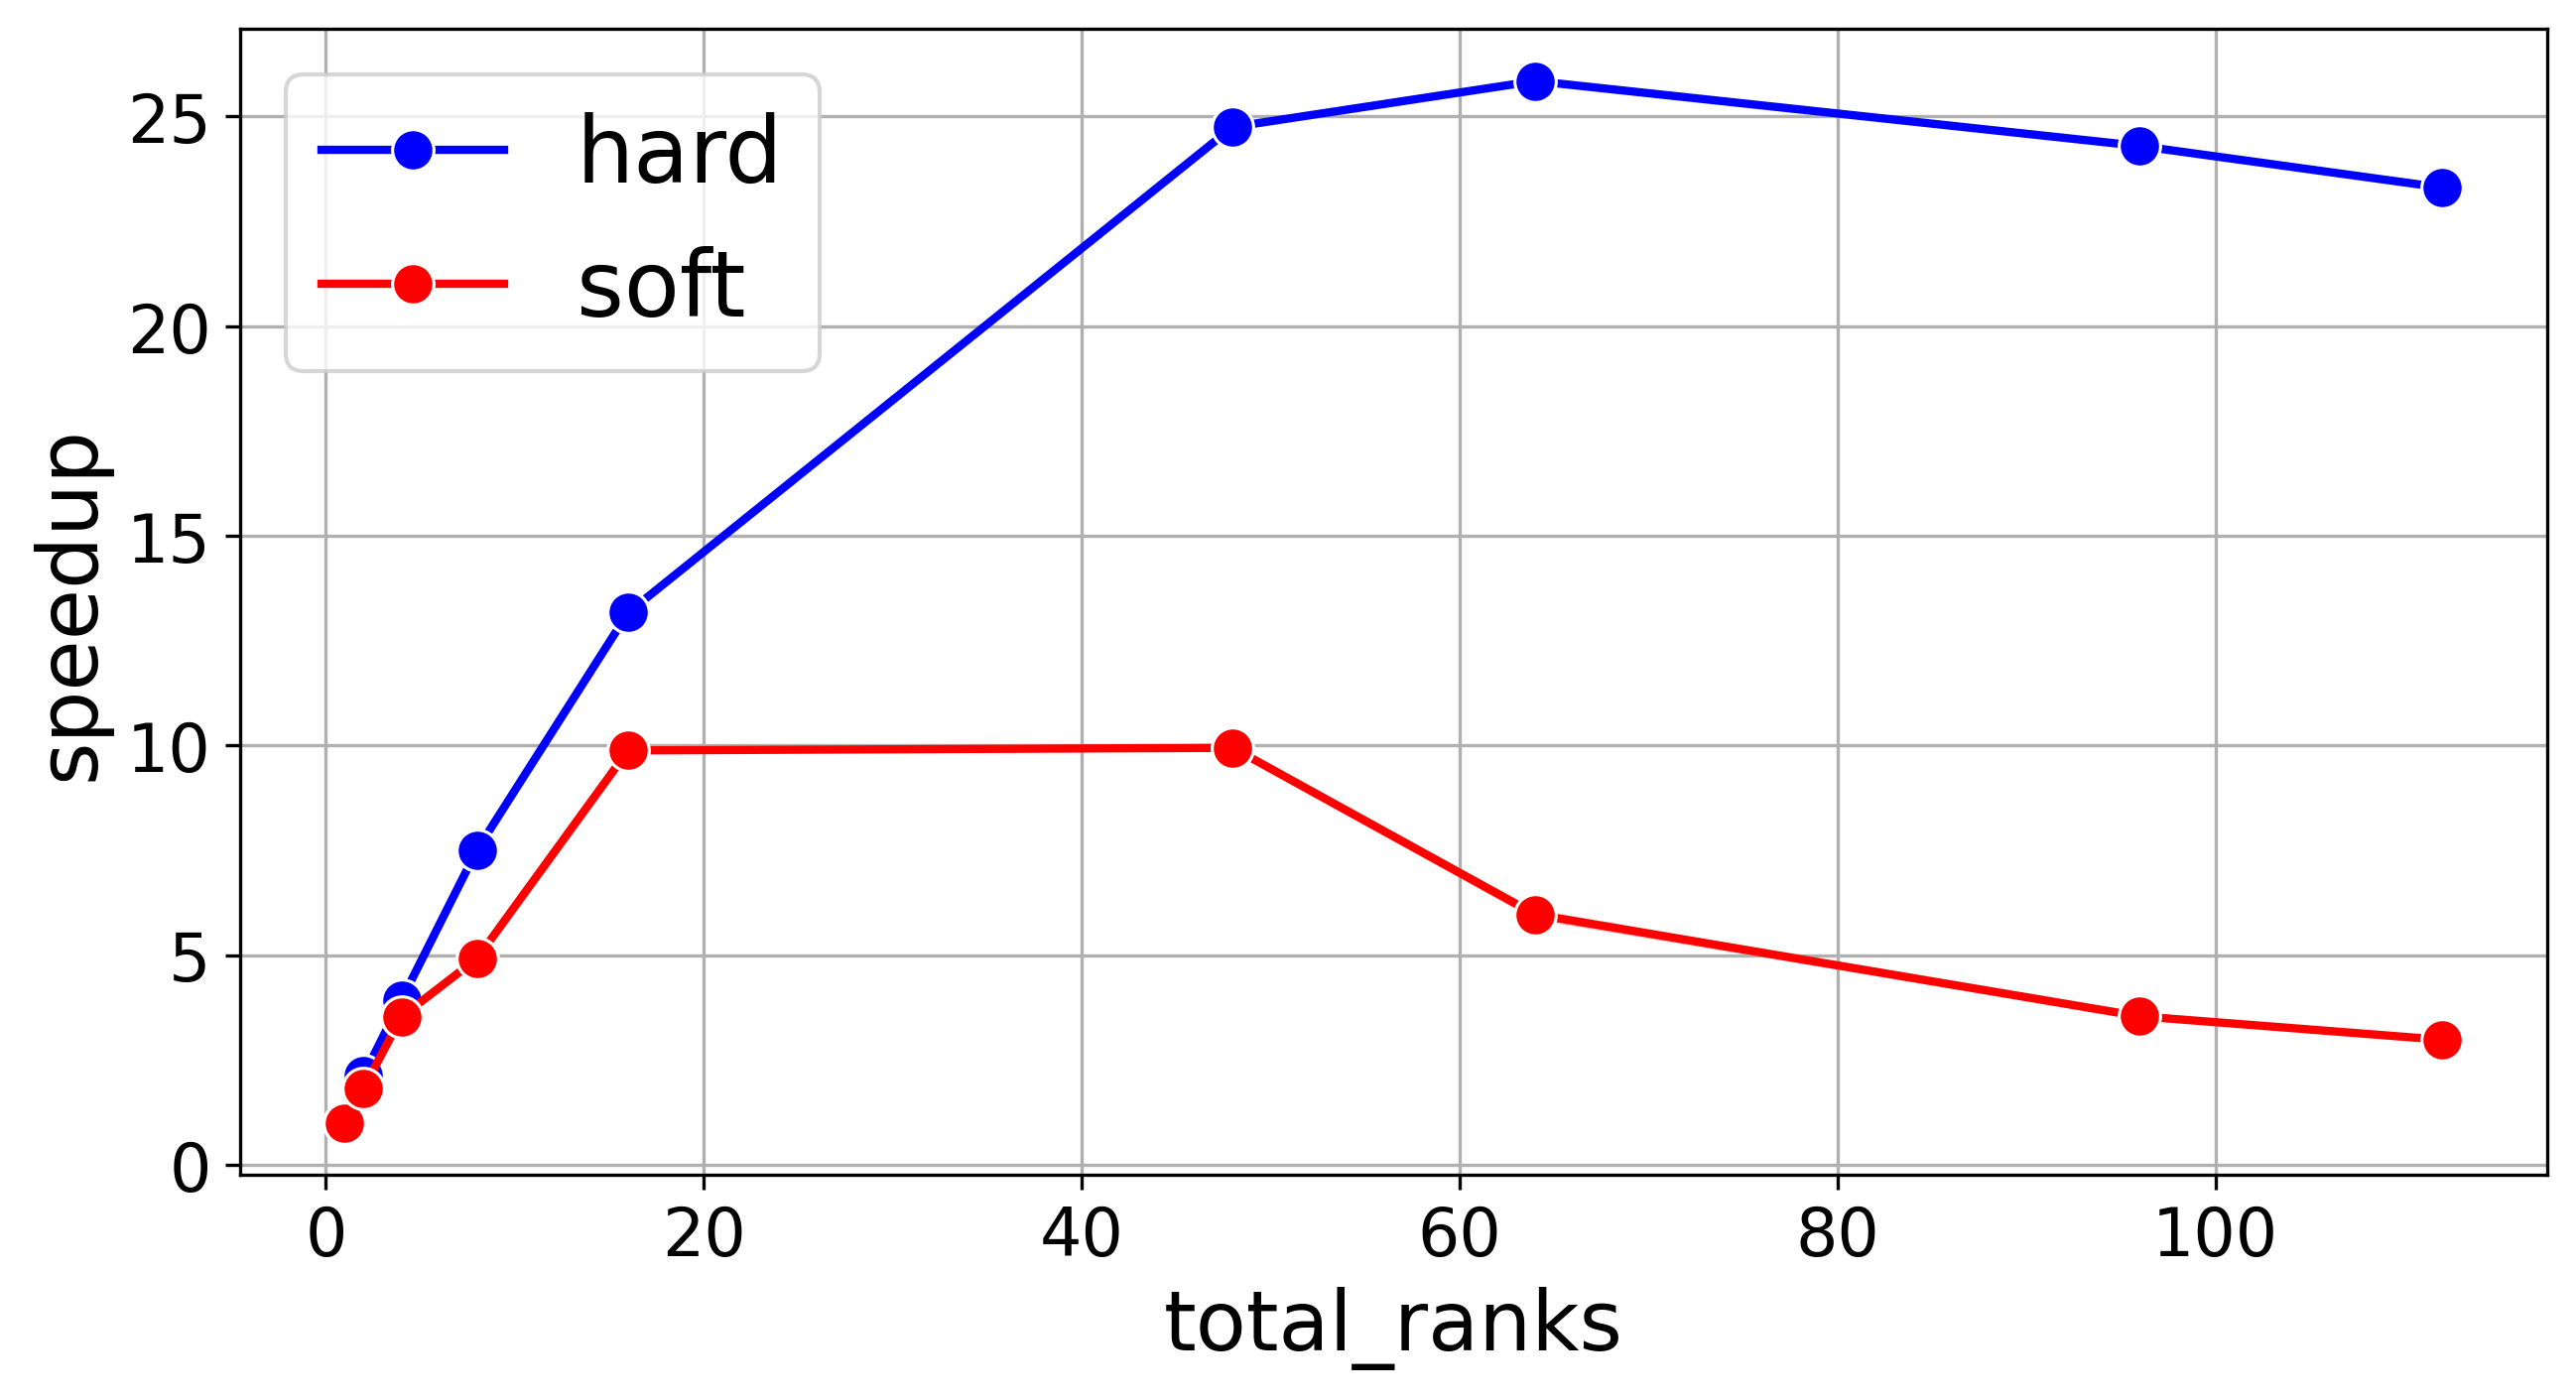
\includegraphics[width=\linewidth]{figures/runtimes/strong_scaling_speedup_hard_soft.png}
        \caption{Speedup versus CPU cores demonstrating Amdahl's Law behavior. Both models fall far below ideal linear scaling due to sequential bottlenecks. Speedup is defined as $S = T_1 / T_r$, where $T_1$ is the runtime on 1 core and $T_r$ is the runtime on $r$ cores.}
        \label{fig:speedup_hard_soft}
    \end{subfigure}

    \caption{Strong scaling comparison. (a) Runtime to reach colony radius of 100. (b) Speedup versus CPU cores.}
\end{figure}

\subsection{Model Efficiency: Walltime and Interaction Overhead}
\label{sec:complexity_scalability}

As shown in \autoref{fig:walltime_per_particle}, the per-particle walltime, defined as the simulation step time divided by the number of particles, is consistently lower for the soft model by roughly two orders of magnitude compared to the hard model. This reflects the soft model's simpler, local force evaluations, in contrast to the hard model's global constraint-solving step.

For the soft model, per-particle walltime decreases as the simulation progresses, as a direct result of improved load balancing. In contrast, the hard model shows a slight increase in per-particle walltime over time, likely caused by the growing complexity of global constraint resolution as more particles interact and more BBPGD iterations are required to find feasible solutions.

Another key factor is the computational load from collision handling (see \autoref{fig:num_constraints}). The soft model processes roughly 6 cell interactions per cell at dense packing levels, consistent with resolving local pairwise interactions. In contrast, the hard model generates approximately 21 constraints per cell due to the ReLCP procedure, which iteratively identifies and resolves newly formed overlaps until all are eliminated. This higher constraint density means the matrices and vectors involved in the optimization problem become larger, leading to increased computational cost per step.


\begin{figure}[h]
    \centering
    \begin{subfigure}[b]{0.9\linewidth}
        \centering
        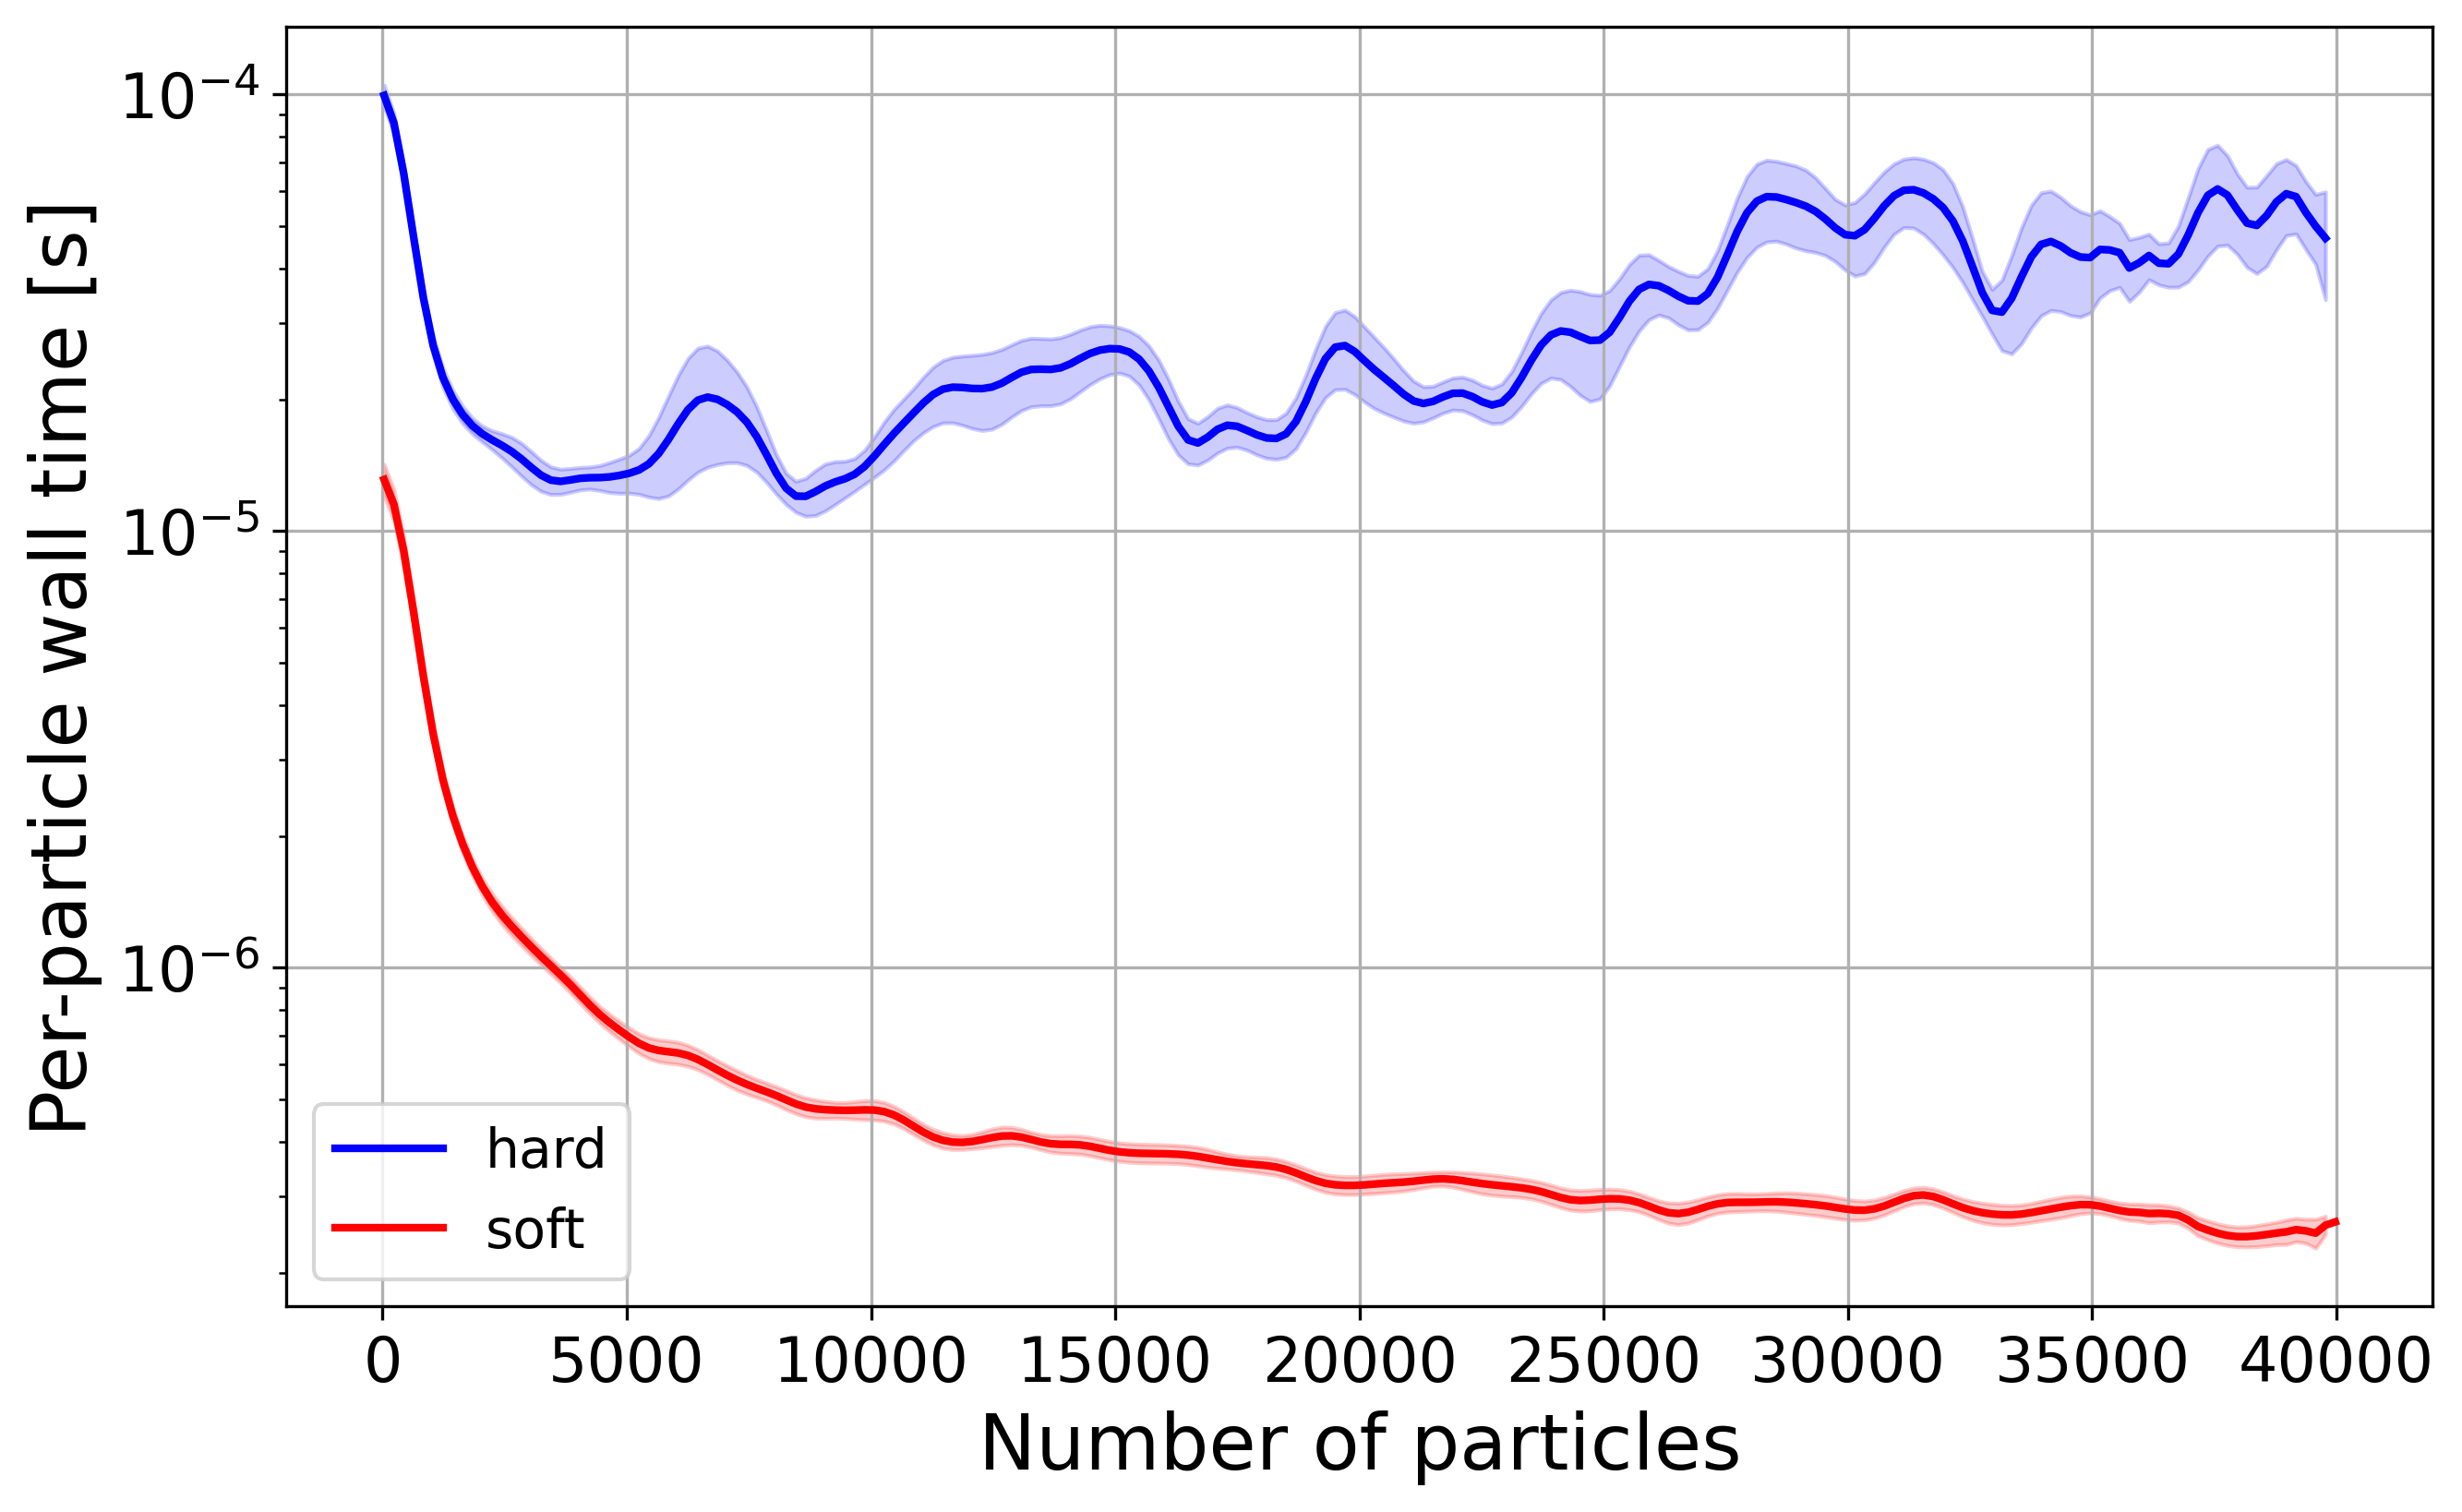
\includegraphics[width=\linewidth]{figures/comparison_plots/combined_num_particles_vs_wall_time_per_particle_with_fit.png}
        \caption{Per-cell walltime for both models with 112 ranks.}
        \label{fig:walltime_per_particle}
    \end{subfigure}

    \begin{subfigure}[b]{0.9\linewidth}
        \centering
        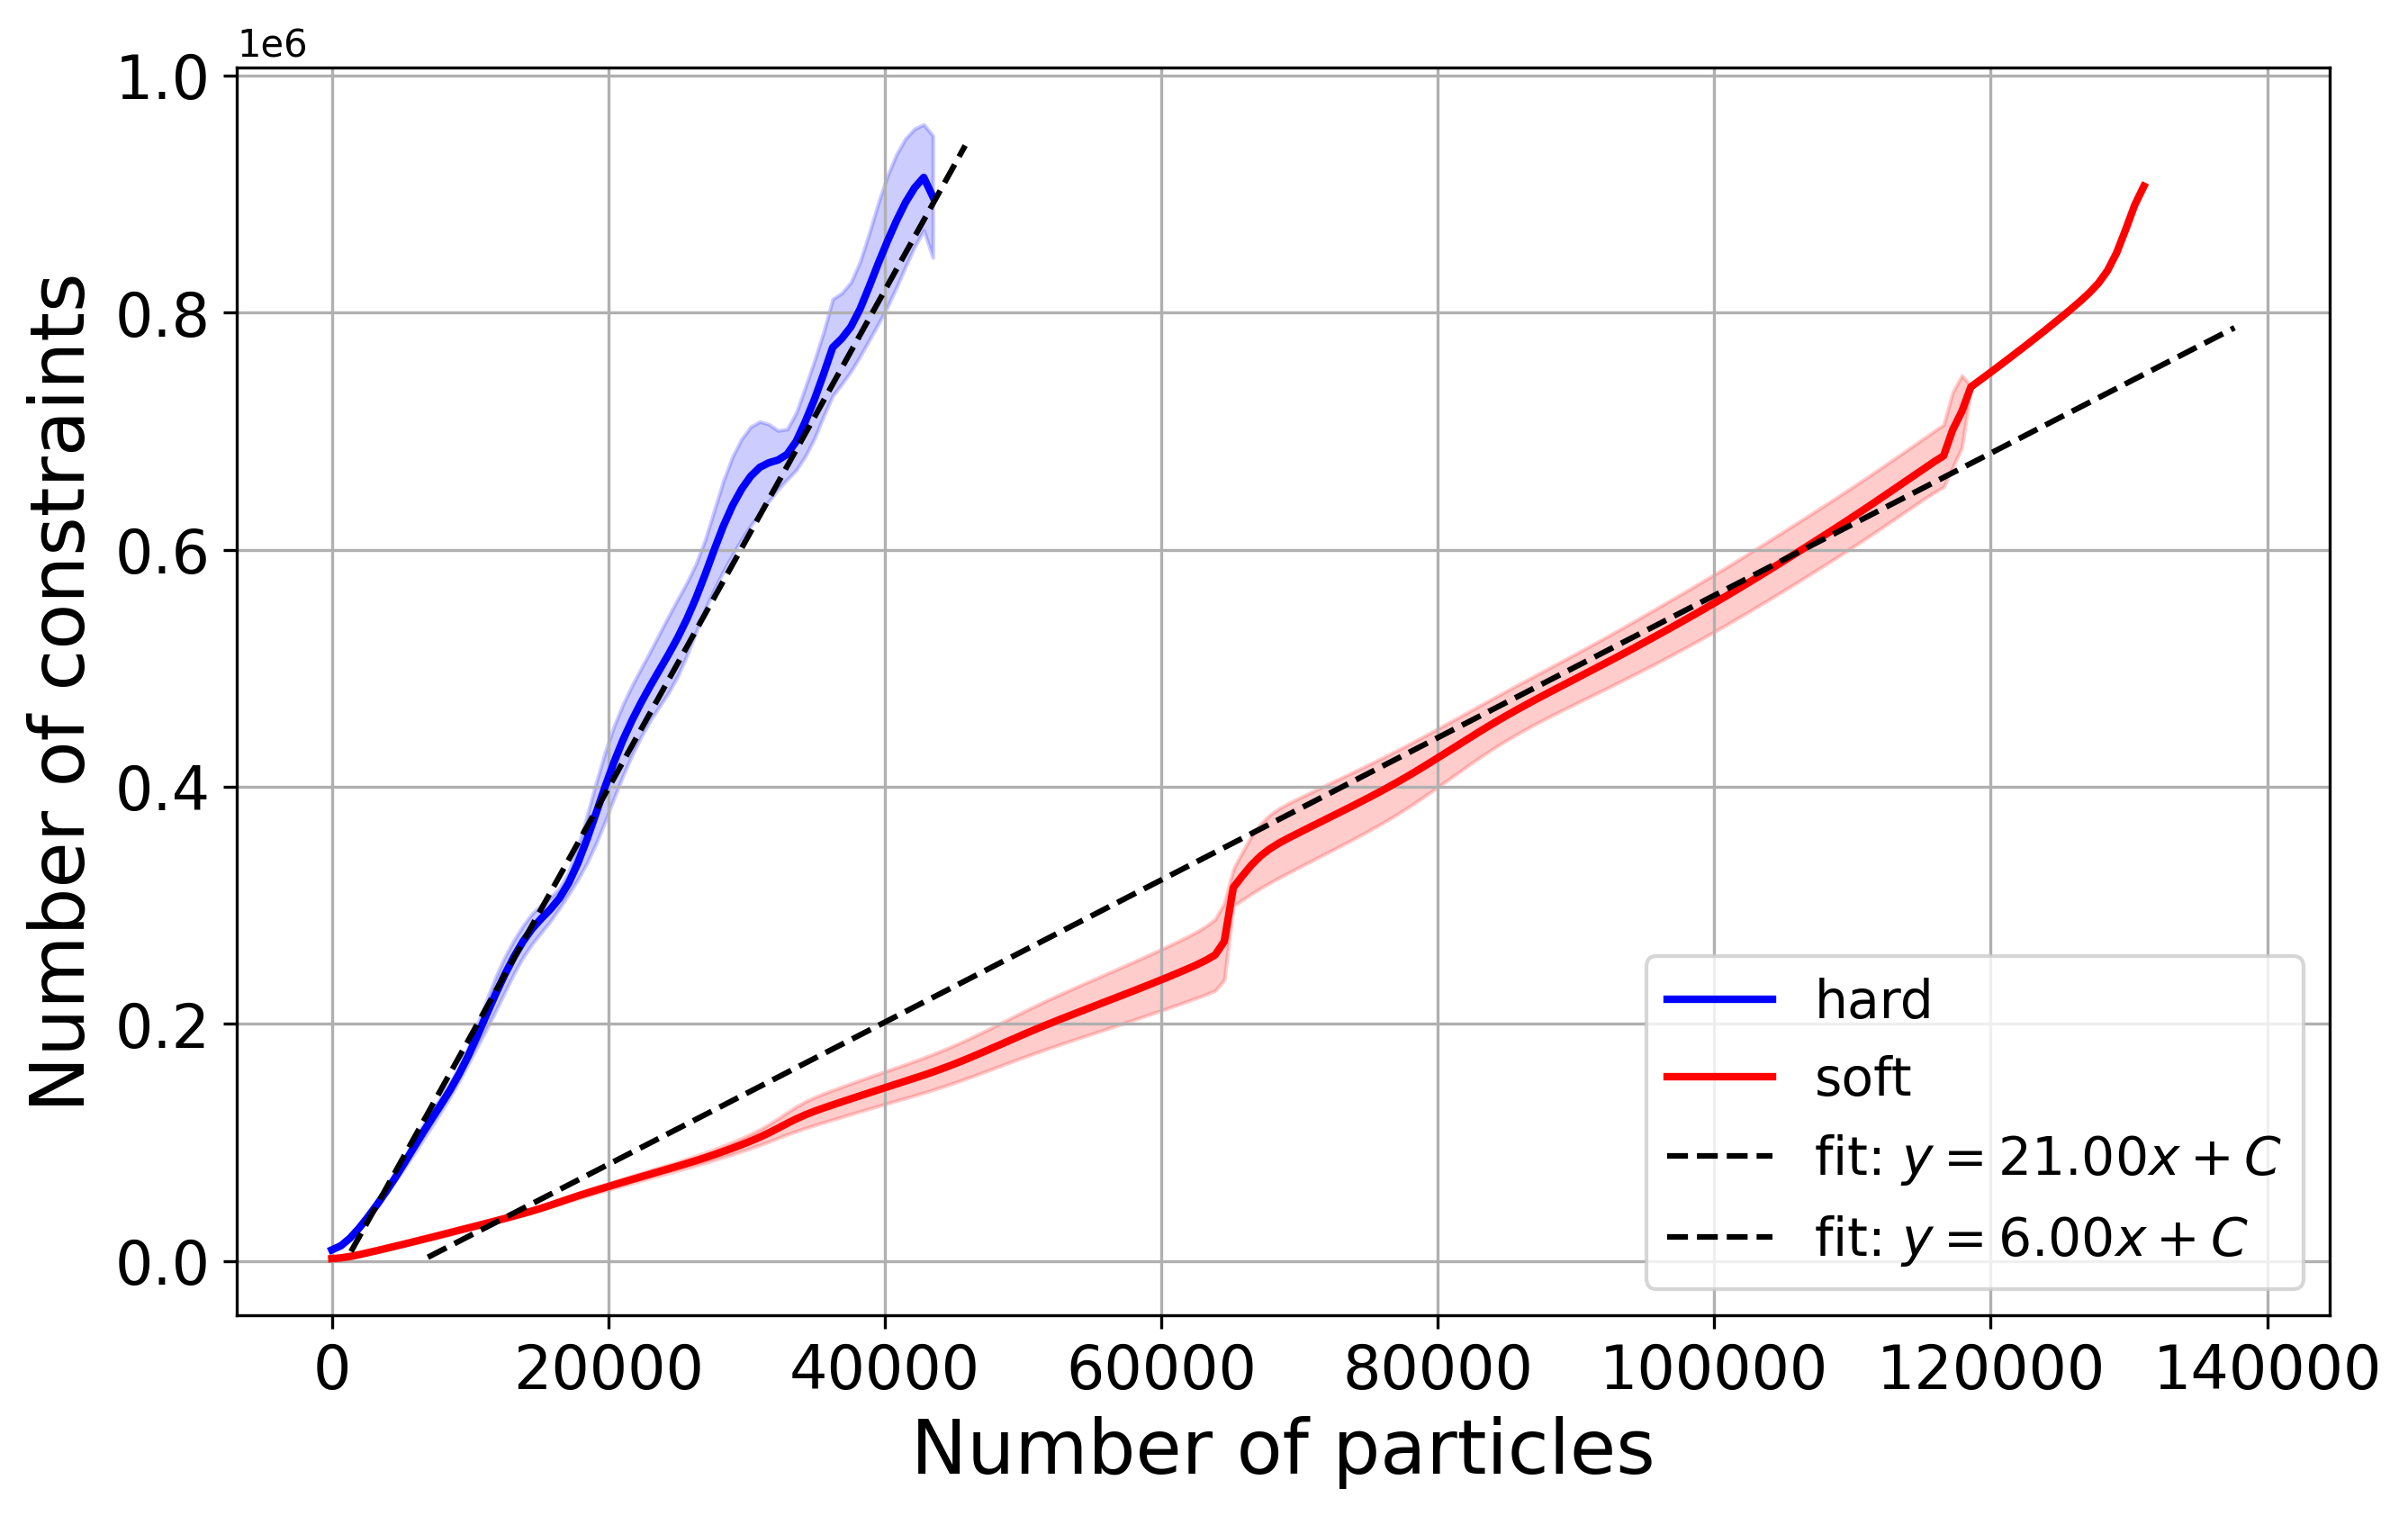
\includegraphics[width=\linewidth]{figures/comparison_plots/combined_num_constraints_vs_num_particles_with_fit.png}
        \caption{Number of cell-cell interactions for both models.}
        \label{fig:num_constraints}
    \end{subfigure}

    \caption{Model efficiency comparison. (a) Per-cell walltime versus number of particles. (b) Number of cell-cell interactions versus number of particles.}
    \label{fig:comparison_metrics}
\end{figure}

\subsection{Impact of Adaptive Timestep on BBPGD Performance}
\label{sec:cfl_analysis}

The efficiency of the BBPGD solver depends strongly on the chosen timestep size, which governs both the number of BBPGD solver iterations per timestep and the total number of timesteps required. This trade-off gives rise to a characteristic U-shaped runtime curve with respect to the CFL number, as shown in \autoref{fig:cfl_vs_runtime}, motivating the use of adaptive timestepping strategies.

As shown in \autoref{fig:cfl_vs_runtime}, the total runtime to reach a colony radius of 100 on 112 CPU cores exhibits a pronounced minimum at CFL $\approx 2$, corresponding to cells moving roughly twice the solver tolerance $\epsilon$ per timestep.

The U-shaped trend arises from competing effects. At small CFL values (CFL $\ll 1$), each timestep requires very few solver iterations due to highly accurate constraint linearization (\autoref{eq:phi_expanded}) and small overlaps, but the simulation remains inefficient overall because a large number of timesteps is required.

Conversely, at large CFL values (CFL $\gg 3$), the linearization assumptions break down as cells move too far per step, causing the approximation of $\mathbf{\Phi}^{k+1}(\boldsymbol{\gamma})$ to deviate from actual separations. This substantially increases the number of solver iterations required to reach feasibility, and in extreme cases (CFL $> 3.7$), the solver may fail to converge entirely, as indicated by the red shaded region in \autoref{fig:cfl_vs_runtime}.

The optimal operating point at CFL $\approx 2$ balances these effects: timesteps are large enough to minimize the total number of timestep yet small enough to maintain linearization accuracy and solver stability.

The figure also shows the average number of solver iterations per timestep, which increases approximately linearly with CFL at low values, following $\text{iterations} \approx 1800 \cdot \text{CFL}$. At the optimal CFL factor of 2, the solver requires around 3600 iterations per physical step on average, after which iteration counts rise sharply, reflecting the deteriorating accuracy of the linearized constraints.

\vfill

\begin{figure}[h]
    \centering
    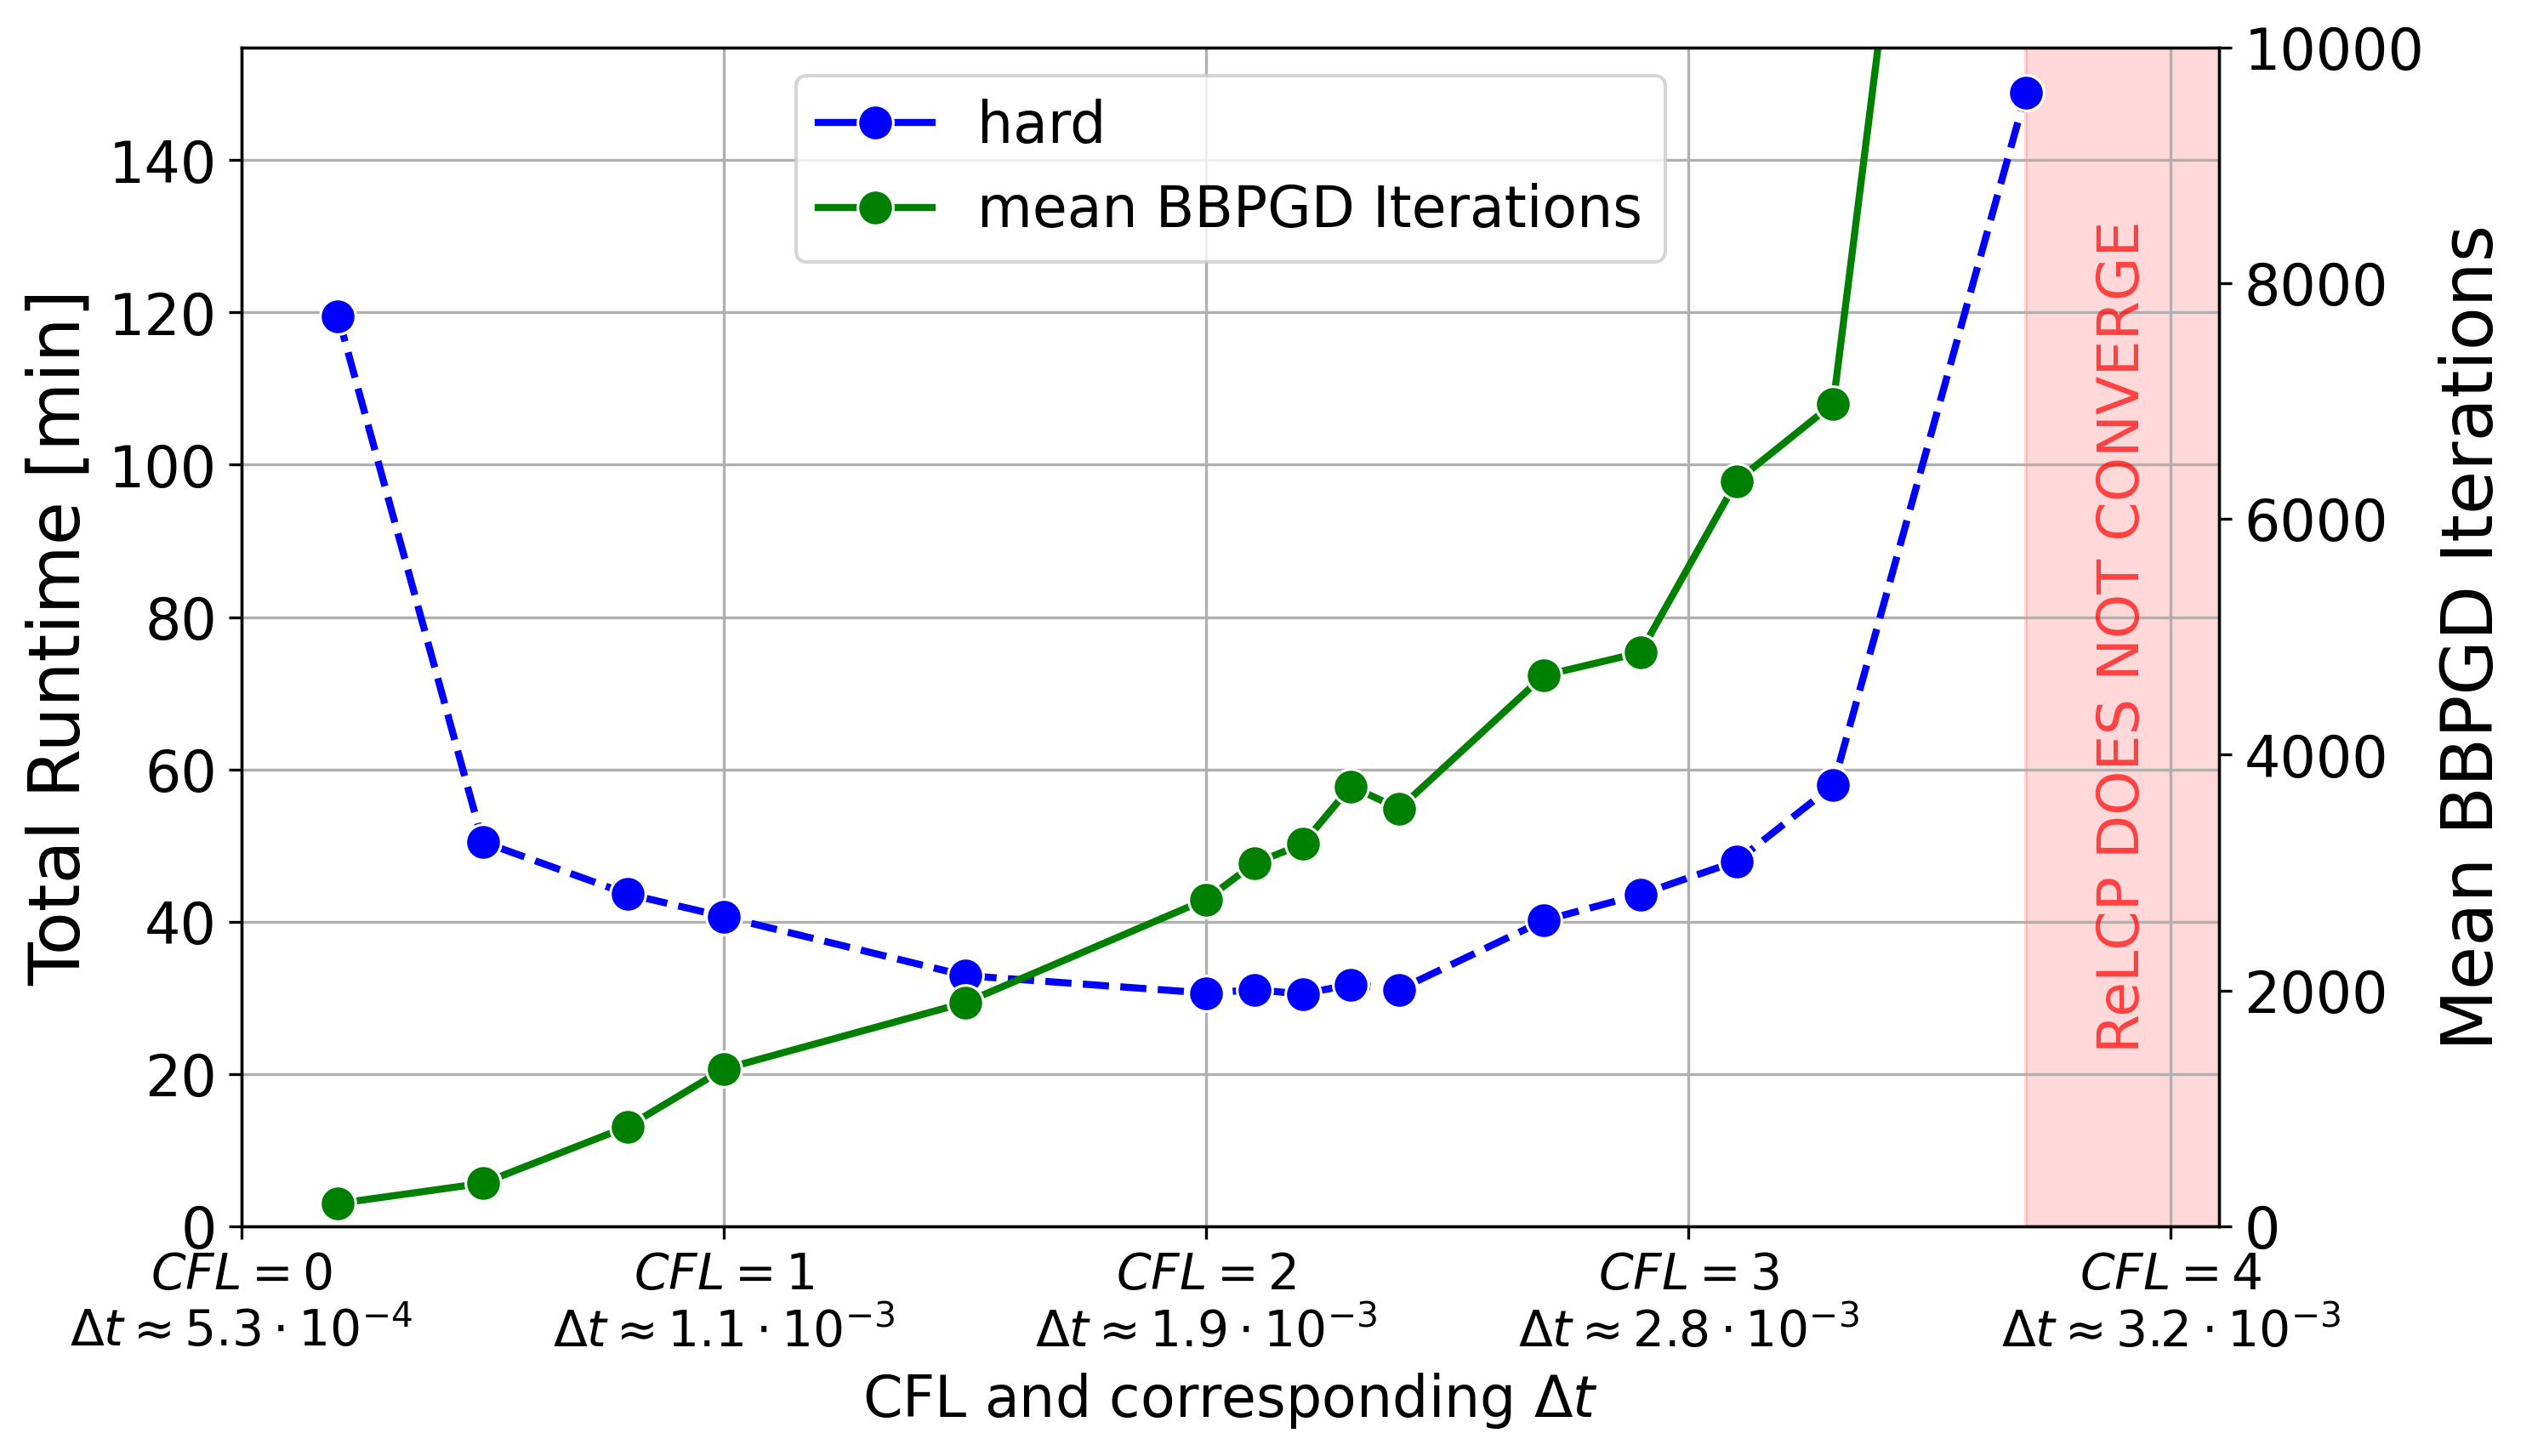
\includegraphics[width=\linewidth]{figures/bbpgd/cfl_vs_runtime_and_constraints.png}
    \caption{Total runtime to reach a colony radius of 100 versus CFL number on 112 cores. The red region indicates CFL values where the ReLCP procedure fails to converge.}
    \label{fig:cfl_vs_runtime}
\end{figure}

\newpage

\subsection{Insights into BBPGD Iterations}

This section examines the performance of the Barzilai-Borwein projected gradient descent (BBPGD) algorithm used in the hard collision model to solve the constrained optimization problem. Since the BBPGD algorithm is the most computationally demanding part of the simulation, understanding its efficiency and convergence is important. In densely packed systems, where numerous contact constraints must be satisfied, BBPGD and its associated matrix-vector operations account for roughly 85\% of the total simulation time and therefore largely determine overall performance.

A key metric is the number of BBPGD iterations required per simulation step and how this quantity scales with system size. \autoref{fig:bbpgd_iterations_per_step_vs_num_particles} shows that iteration count remains mostly on the order of $\mathcal{O}(1000)$, with occasional peaks reaching $\mathcal{O}(5000)$ during critical moments such as large-scale rearrangements or near jamming transitions. This count includes additional BBPGD calls from the ReLCP~\cite{Weady2024SM} procedure, which requires up to 11 iterations to fully resolve remaining overlaps. The typical order of magnitude for the BBPGD iteration count is consistent with related studies~\cite{Yan2019}, though our model's collision-growth coupling introduces additional complexity.

The convergence behavior of a single BBPGD solve during a representative timestep is illustrated in \autoref{fig:bbpgd_residual}. The solver reaches the desired tolerance of $\epsilon = 10^{-3}$ after approximately 280 iterations. The residual exhibits a highly oscillatory pattern, a well-known characteristic of BBPGD resulting from adaptive step-size selection~\cite{BBPGD,Schneider2021}.

Since the ReLCP procedure~\cite{Weady2024SM} is also employed, each simulation step may involve multiple BBPGD solves until all overlaps are resolved. The overall energy evolution during the convergence process is shown in \autoref{fig:bbpgd_energy}, demonstrating that the solver consistently makes progress until all current overlaps are eliminated. Once this state is reached, new contacts are detected, the systems energy increases, and the process repeats. The system converges to a feasible, overlap-free configuration within six ReLCP iterations, requiring a total of 960 BBPGD iterations.

The plot also shows the total amount of constraints being resolved during the BBPGD iterations, which decreases as the solver progresses. For a colony of size $R \approx 100$ with 36244 cells, approximately 100,000 new constraints are generated per ReLCP iteration, reaching a maximum of around 600,000 constraints in the final phase.

There remains considerable potential to further improve the performance of BBPGD. As demonstrated in \autoref{sec:cfl_analysis}, the timestep size critically influences solver efficiency. Future work could investigate more advanced adaptive schemes that directly leverage solver feedback, for instance by adjusting $\Delta t$ based on the number of BBPGD iterations or the ReLCP convergence rate. Moreover, warm-start techniques that initialize the solver with multipliers from previous timesteps could help reduce iteration counts, particularly in later stages where colony configurations evolve more gradually and inter-cell forces remain relatively stable between steps.

\newpage

\begin{figure}[H]
    \centering
    \begin{subfigure}[b]{\linewidth}
        \centering
        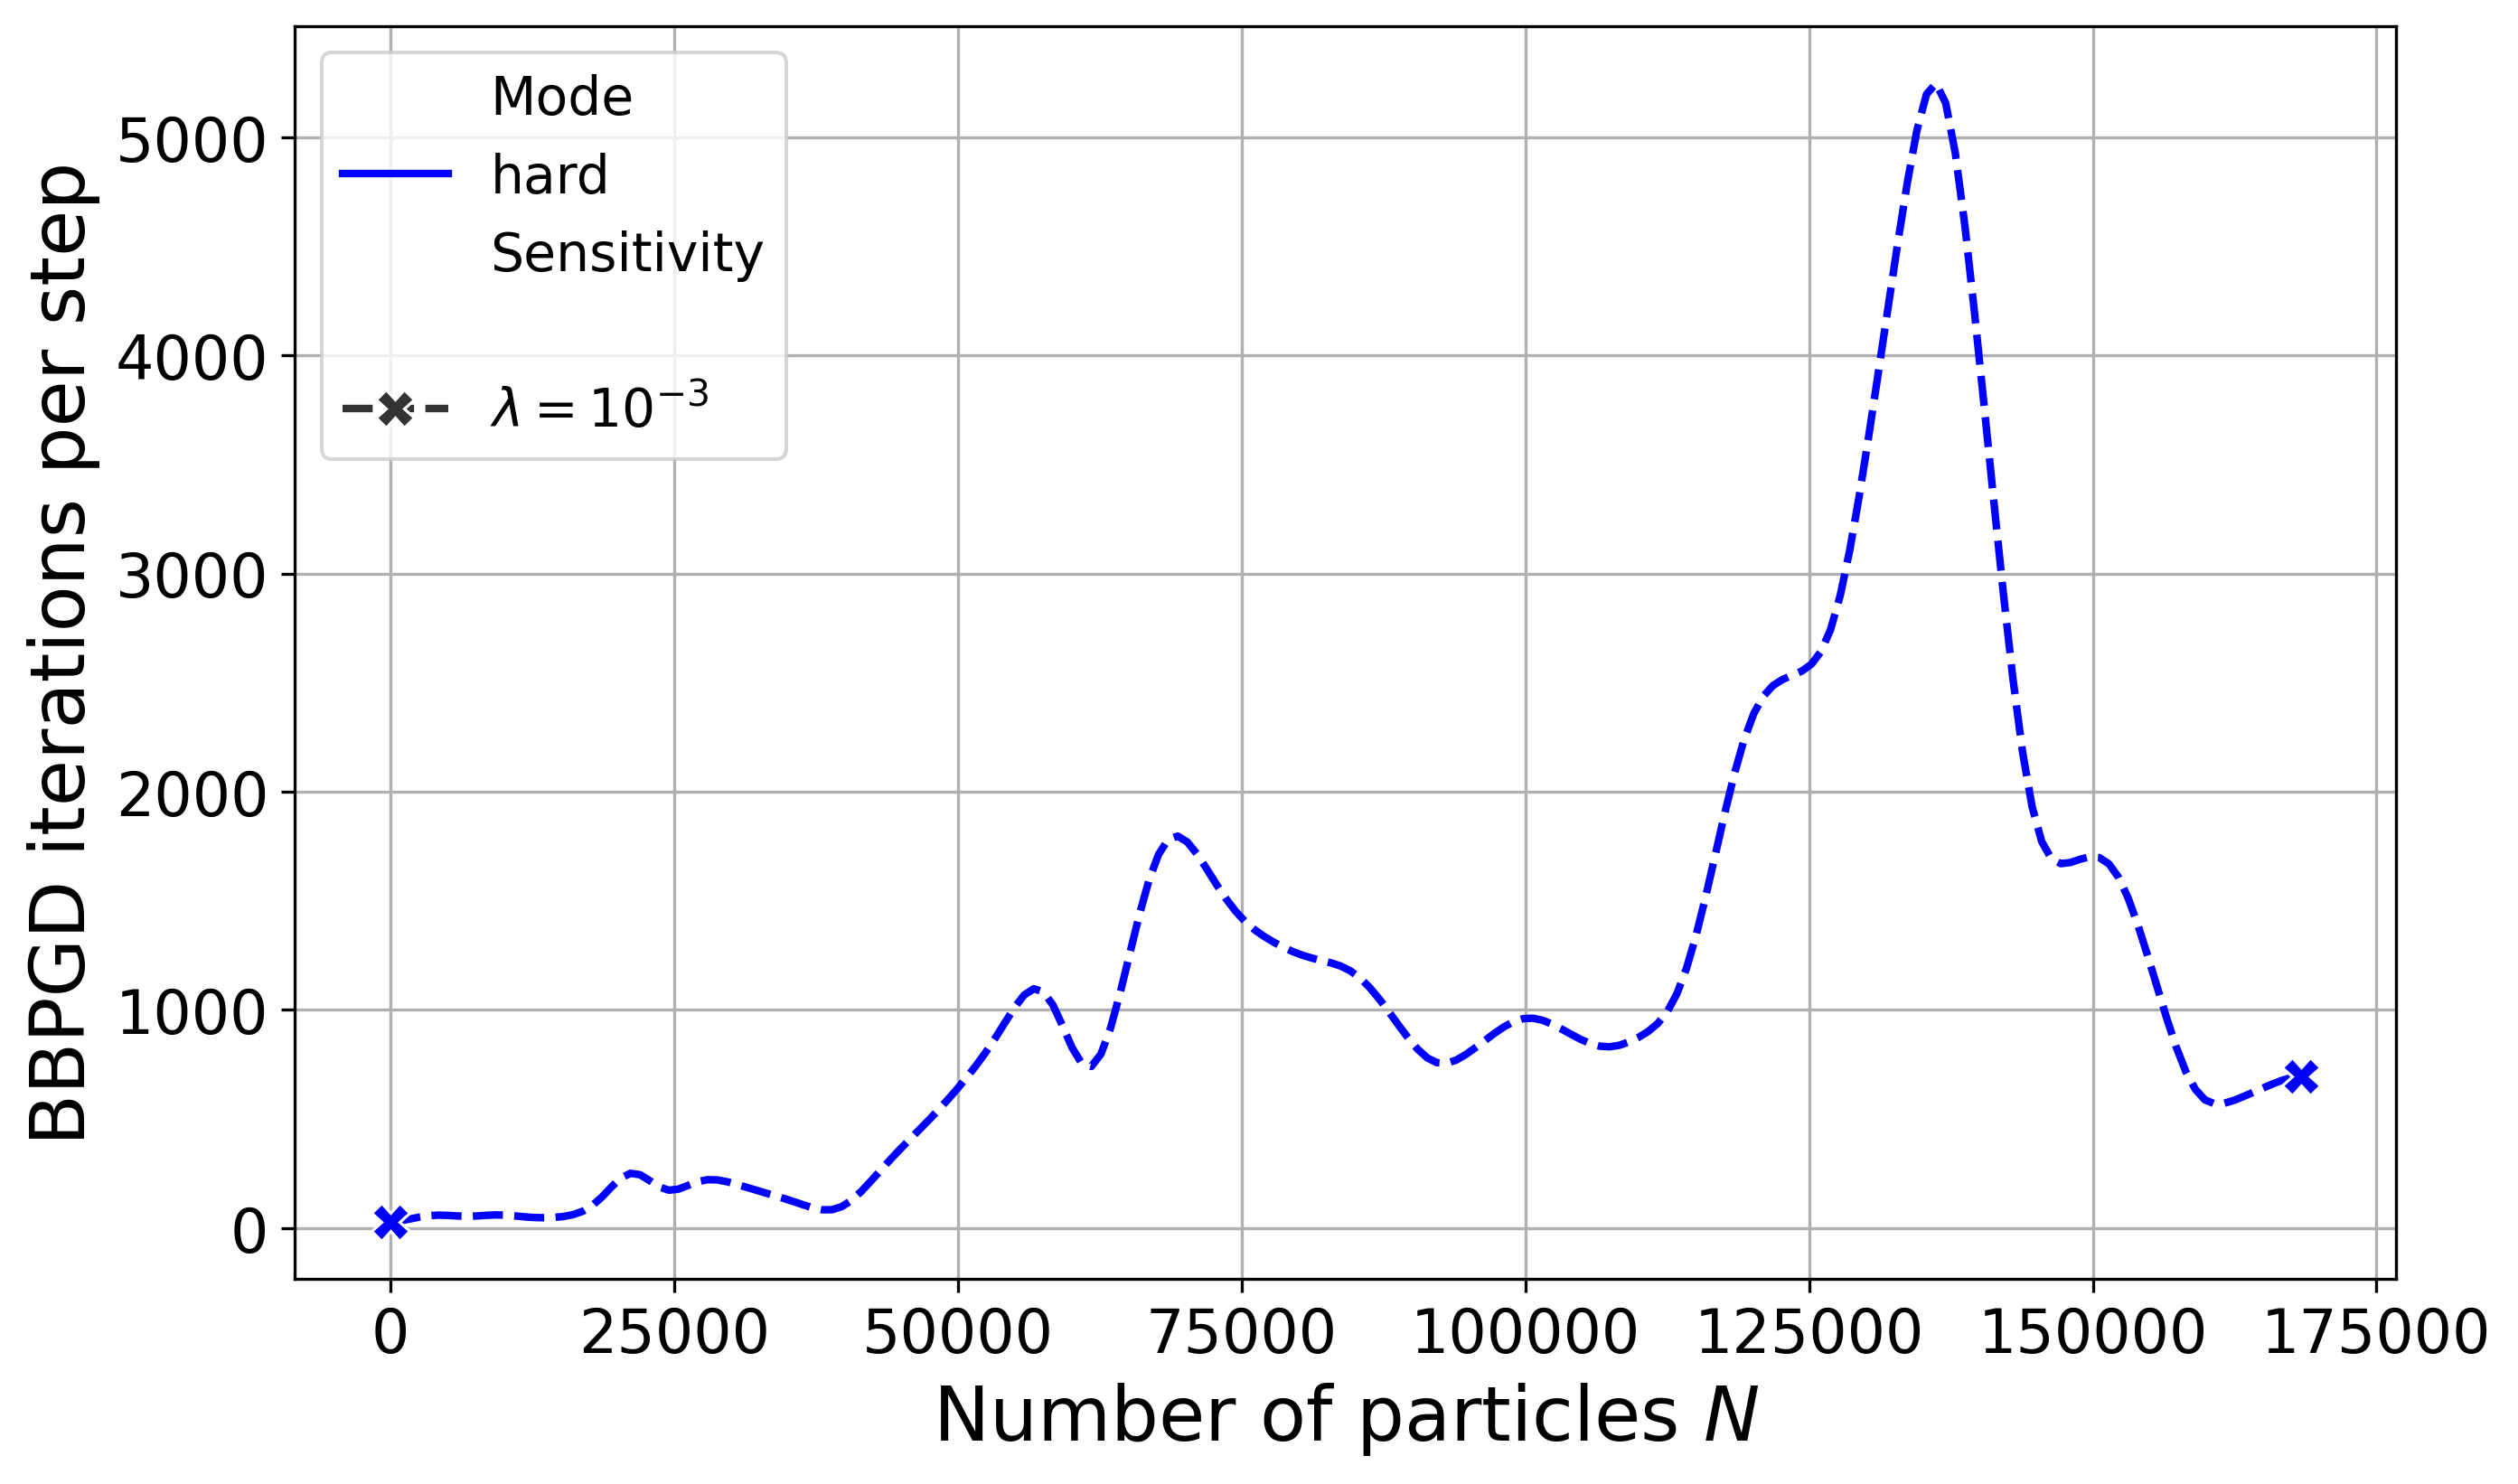
\includegraphics[width=\linewidth]{figures/bbpgd/bbpgd_num_particles_vs_bbpgd_steps.png}
        \caption{Number of BBPGD iterations per timestep as a function of particle count. Iterations remain roughly $\mathcal{O}(1000)$ on average, with occasional spikes up to $\mathcal{O}(5000)$.}
        \label{fig:bbpgd_iterations_per_step_vs_num_particles}
    \end{subfigure}

    \begin{subfigure}[b]{\linewidth}
        \centering
        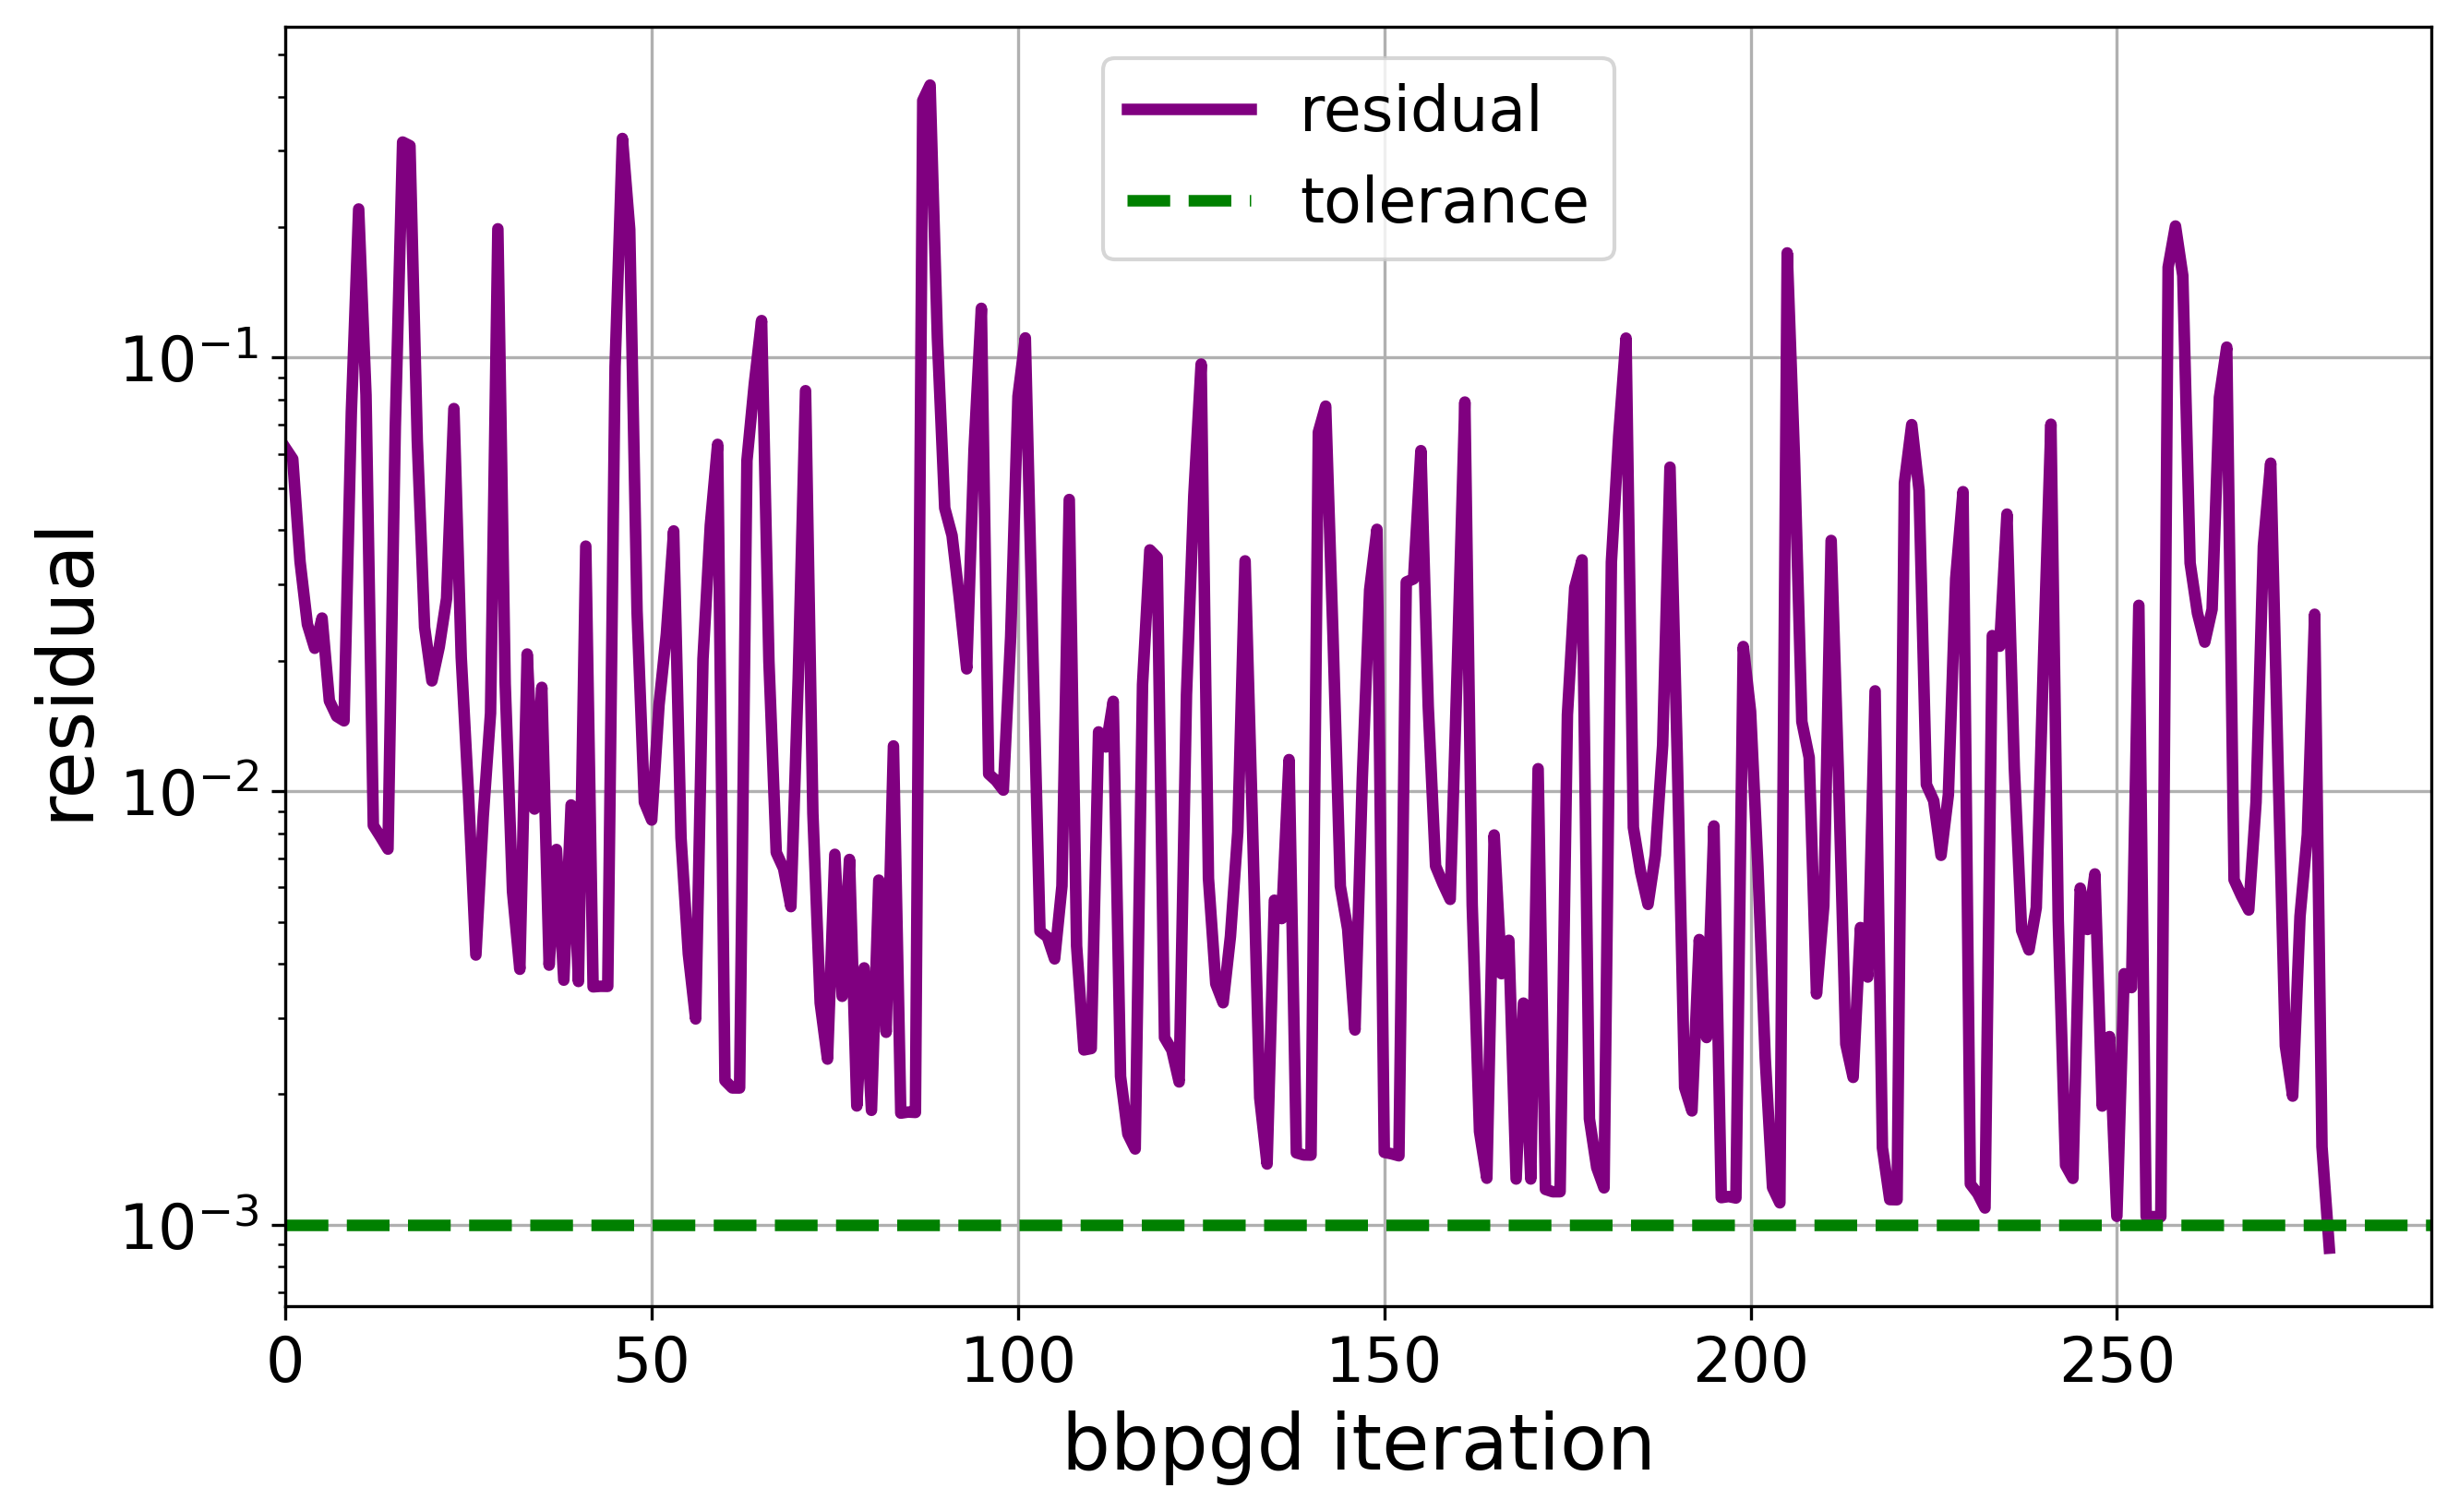
\includegraphics[width=\linewidth]{figures/bbpgd/bbpgd_residual.png}
        \caption{BBPGD residuals over iterations for a single timestep. The solver converges to tolerance $\epsilon = 10^{-3}$ within approximately 280 iterations, showing highly oscillatory behavior. The residual directly represents the current maximum overlap between any two cells in the colony.}
        \label{fig:bbpgd_residual}
    \end{subfigure}

    \begin{subfigure}[b]{\linewidth}
        \centering
        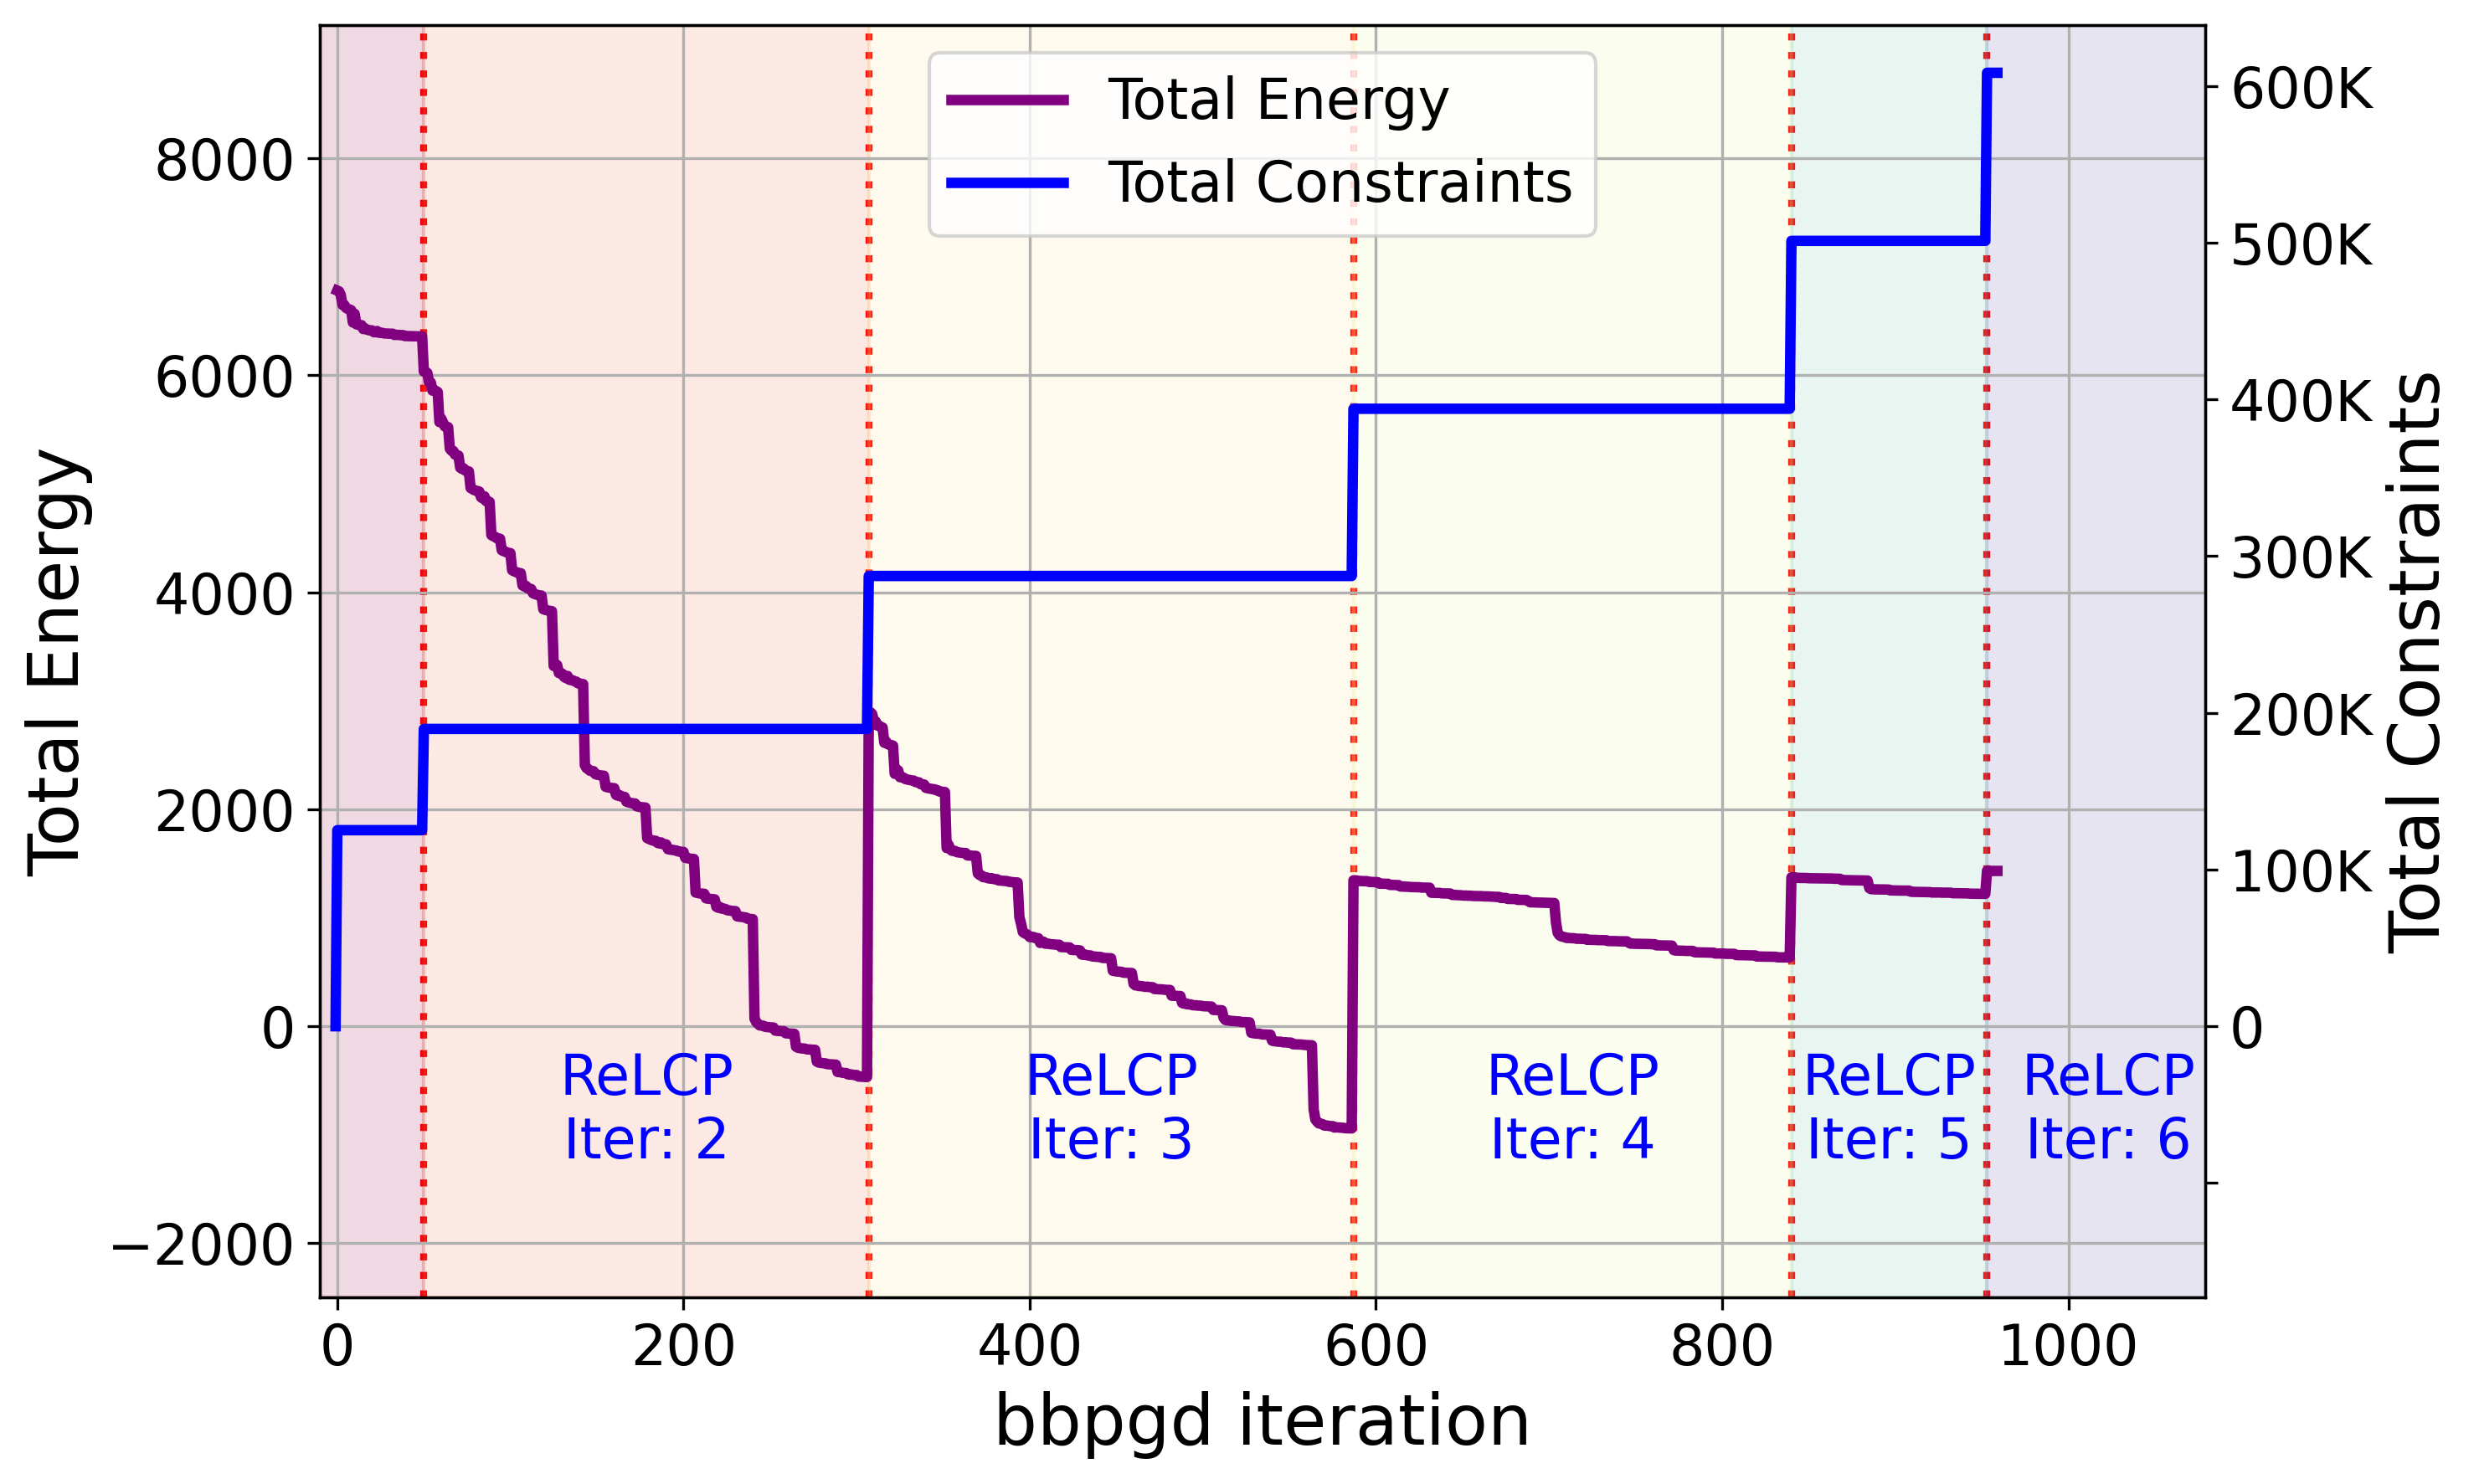
\includegraphics[width=\linewidth]{figures/bbpgd/bbpgd_total_energy.png}
        \caption{System energy (\autoref{eq:energy_function}) throughout the ReLCP procedure during a single timestep. The energy consistently decreases as BBPGD iterations progress. After each set of constraints is resolved, new overlaps are detected, and the process repeats until a feasible configuration is reached within six ReLCP iterations.}
        \label{fig:bbpgd_energy}
    \end{subfigure}

    \caption{BBPGD convergence analysis for a typical timestep in a colony of size $R \approx 100$ with 36244 cells. (a) BBPGD iterations per timestep versus number of particles. (b) Residuals over iterations. (c) System energy over iterations.}
    \label{fig:bbpgd_analysis}
\end{figure}


\subsection{Maximum Attainable Colony Size}
\label{sec:maximum_colony_size}

This section investigates the maximum achievable colony size within a fixed computational budget of 24 hours on 112 CPUs, using a stress sensitivity of $\lambda = 10^{-3}$.

As illustrated in \autoref{fig:huge_wall_time_vs_radius}, the soft model reaches a maximum colony radius of approximately $R = 210$ compared to $R = 195$ for the hard model, despite requiring substantially more particles (approximately 1,033,108 versus 168,339). This demonstrates that the soft model's per-particle efficiency outweighs the cost of simulating additional cells.

Contrary to the strong-scaling results (see \autoref{sec:strong_scaling}), the soft model becomes increasingly advantageous for colony sizes beyond $R = 100$, with the wall-time curves diverging at larger radii, as illustrated in \autoref{fig:huge_wall_time_vs_radius}.

Despite the observed differences in stress distribution, the macroscopic structure of the colonies remains largely comparable between the two models, even at large sizes. As shown in \autoref{fig:huge_length_shared}, the average radial cell length exhibits nearly identical oscillatory patterns, suggesting that variations in microscopic density and local interactions have little effect on the emergent macroscopic ring structures.

A representative snapshot of the colony at its maximum size for the hard model is provided in \autoref{fig:huge_colony_hard}.

\begin{figure}[h]
    \centering
    \begin{subfigure}[b]{0.9\linewidth}
        \centering
        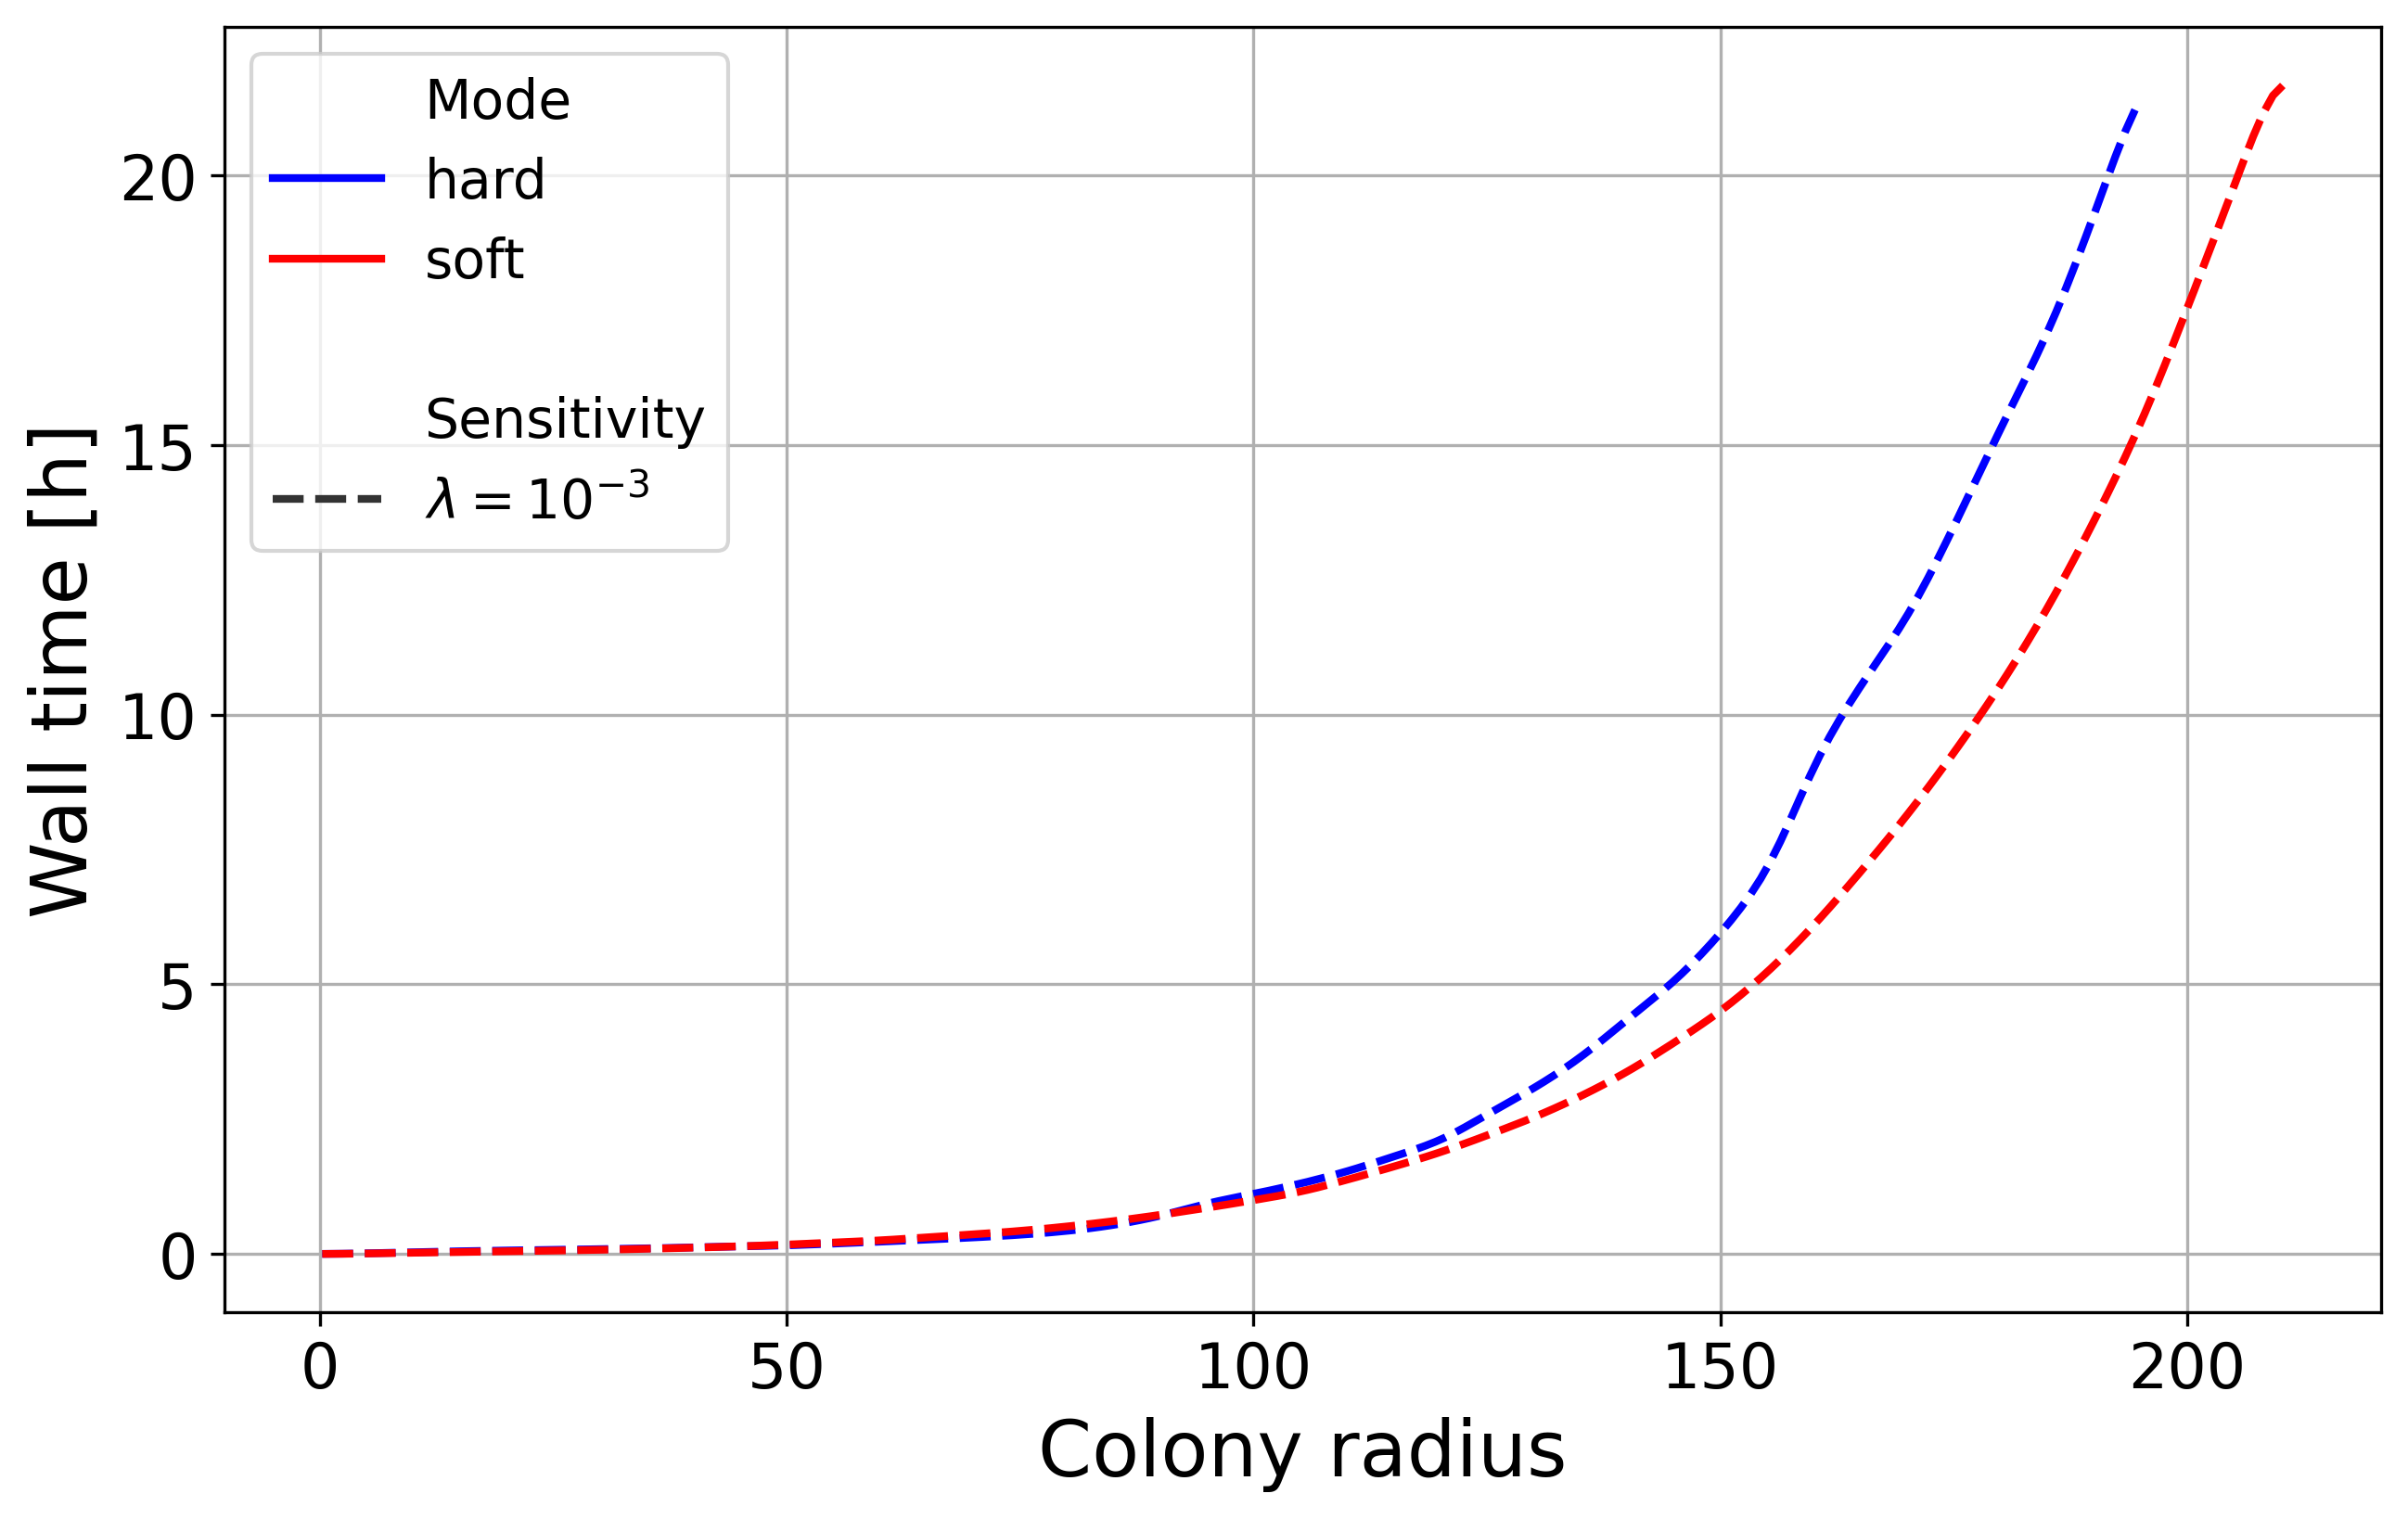
\includegraphics[width=\linewidth]{figures/comparison_plots/huge_wall_time_vs_radius.png}
        \caption{Colony radius over wall time for both models.}
        \label{fig:huge_wall_time_vs_radius}
    \end{subfigure}

    \begin{subfigure}[b]{0.9\linewidth}
        \centering
        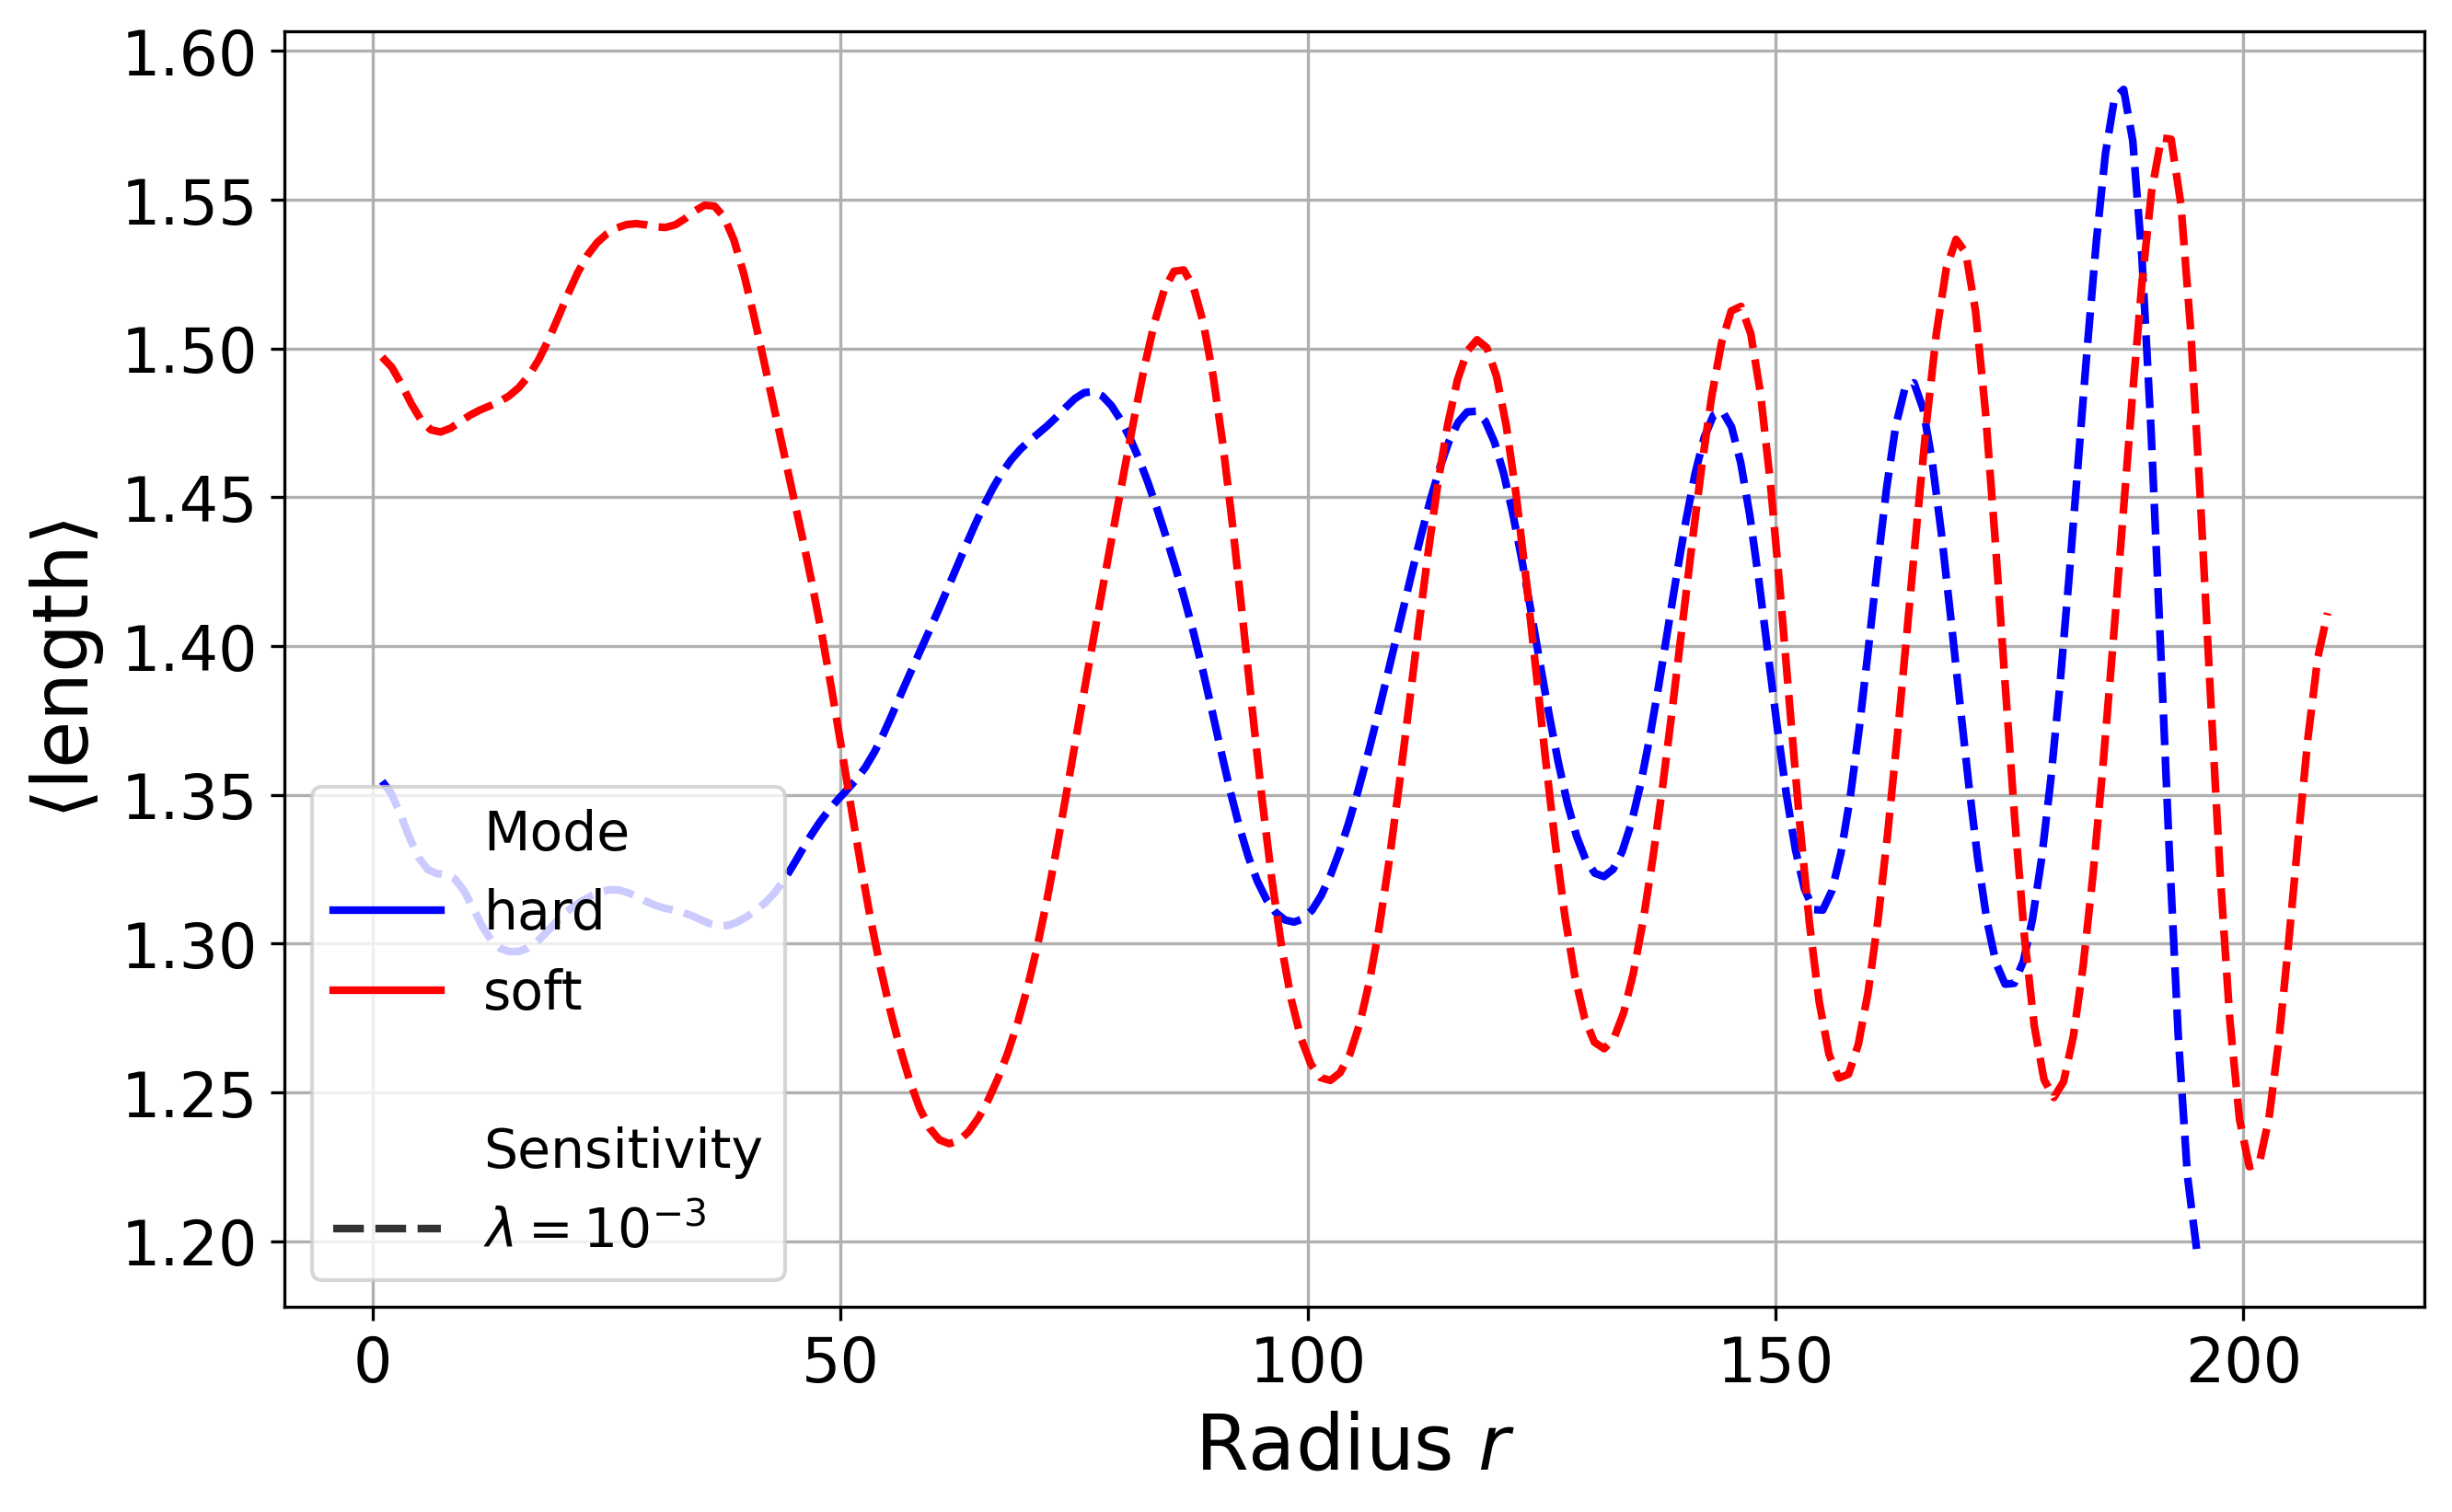
\includegraphics[width=\linewidth]{figures/comparison_plots/huge_length_shared.png}
        \caption{Average cell length $\langle \text{length} \rangle$ versus colony radius.}
        \label{fig:huge_length_shared}
    \end{subfigure}

    \caption{Large-scale colony growth comparison. (a) Colony radius versus wall time. (b) Average cell length versus radius at maximum colony size.}
\end{figure}

\clearpage
\newpage

\section{Discussion and Conclusion}

This work presented a systematic comparison of hard (constraint-based) and soft (potential-based) collision models for simulating proliferating cell collectives, implemented within a unified computational framework. Our investigation yielded several key insights that clarify the trade-offs between these two dominant modeling paradigms.

We demonstrated that both models successfully reproduce the concentric ring patterns and microdomain formation observed in experimental bacterial colonies, confirming that these macroscopic phenomena are emergent properties of growth-mechanics feedback and are robust to the specific details of collision resolution. This robustness is a significant finding, as it justifies the use of computationally cheaper models for studies focused on colony-level pattern formation.

Beneath this macroscopic similarity lie critical microscopic differences. The hard model enforces strict non-overlap, maintaining a realistic packing fraction of about 0.9 and producing reliable stress distributions and microdomain structures. In contrast, the soft model cannot fully reproduce continuum-theory stress profiles and allows significant, unphysical cell overlap. This results in packing fractions exceeding 5 in colony centers, distorting microdomain morphology and producing elongated, unrealistic cell bundles, particularly in large colonies or under low stress-sensitivity conditions.

Our performance benchmarking revealed a clear computational trade-off. The hard model's ability to use timesteps approximately 30 times larger than the soft model ($\Delta t_{\text{hard}} \approx 3 \times 10^{-4}$ h vs. $\Delta t_{\text{soft}} \approx 10^{-5}$ h) is offset by its higher per-step cost, at large colony sizes. Consequently, the hard model outperforms the soft model only for small to moderate colonies ($R \leq 100$), while the soft model's superior per-particle efficiency enables it to simulate much larger colonies (up to $R \approx 210$) within the same computational budget.

The introduction of an adaptive timestepping algorithm based on the Courant-Friedrichs-Lewy condition proved essential for maintaining numerical stability in both models, dynamically selecting stable timesteps tailored to the current colony state.

In summary, the decision between hard and soft collision models mostly depends on the goals of the study rather than absolute performance. The soft model offers an efficient and biologically reasonable option for large-scale investigations of macroscopic pattern formation, where exact geometric fidelity is less critical. It performs particularly well when simulating very large colonies or when computational resources are limited. Conversely, the hard model is preferred when accurate stress distributions, precise cell packing, or faithful microdomain structures are essential.

Choosing the appropriate model, therefore, requires balancing computational efficiency against the level of microscopic detail needed for the study.

\newpage

\section{Future Work}

The computational challenges identified in this work suggest several promising research directions to enhance the scale and efficiency of simulating proliferating cell collectives. While our current implementation provides a solid foundation, significant optimizations remain to exploit modern HPC architectures fully.

\subsection{Adaptive Resource Allocation for Early-Stage Simulations}

A key limitation in our current parallel implementation is the inefficient resource utilization during the initial growth phases. While dynamic load balancing distributes cells evenly across ranks, most MPI ranks remain largely empty until the colony reaches a substantial size. Future work should investigate adaptive resource strategies that begin with fewer, more densely populated ranks and dynamically scale up the active processor count as the colony expands. This could involve implementing a work-stealing approach where idle ranks temporarily assist overloaded ones, or developing a hierarchical domain decomposition that initially partitions at a coarser granularity.

\subsection{GPU Acceleration via PETSc}

The computational bottleneck of the hard model, particularly for large colonies, is the BBPGD solver. Building on the work of~\cite{Tasora2008}, who demonstrated the effectiveness of GPU acceleration for similar constraint-based models, future work could leverage PETSc's built-in GPU support. PETSc enables seamless offloading of linear algebra operations to GPUs through simple runtime configuration, requiring minimal code changes. This approach has been shown to provide significant performance improvements for large-scale simulations where the constraint solver dominates computational cost~\cite{Tasora2008}.

\subsection{Usage of Molecular Dynamics Libraries for the Soft Model}

The soft collision model's pairwise force calculations are computationally very similar to those used in molecular dynamics, suggesting that it could greatly benefit from leveraging specialized libraries like AutoPas~\cite{Gratl2019,Newcome2023}. These libraries are already highly optimized and well-benchmarked, offering efficient neighbor search algorithms, automatic selection of data structures (e.g., Verlet lists or cell lists), and hardware-aware traversal schemes. Integrating the soft model into AutoPas could therefore improve performance and enable automatic tuning of simulation parameters, without requiring extensive custom optimization.

\section*{Acknowledgments}

We gratefully acknowledge the computational and data resources, as well as the support provided by the Leibniz Supercomputing Centre (\url{www.lrz.de}). All benchmarks in this work were carried out on the \texttt{CoolMUC-4} cluster, which is part of the Linux Cluster at LRZ. Further information is available at \url{https://doku.lrz.de/coolmuc-4-1082337877.html}.


\newpage

\balance
\bibliographystyle{IEEEtran}
\bibliography{literature}
\newpage
\nobalance


\onecolumn

\appendix
\renewcommand{\thefigure}{A\arabic{figure}}
\renewcommand{\thetable}{A.\arabic{table}}
\setcounter{figure}{0}
\setcounter{table}{0}


\begin{figure}[H]
    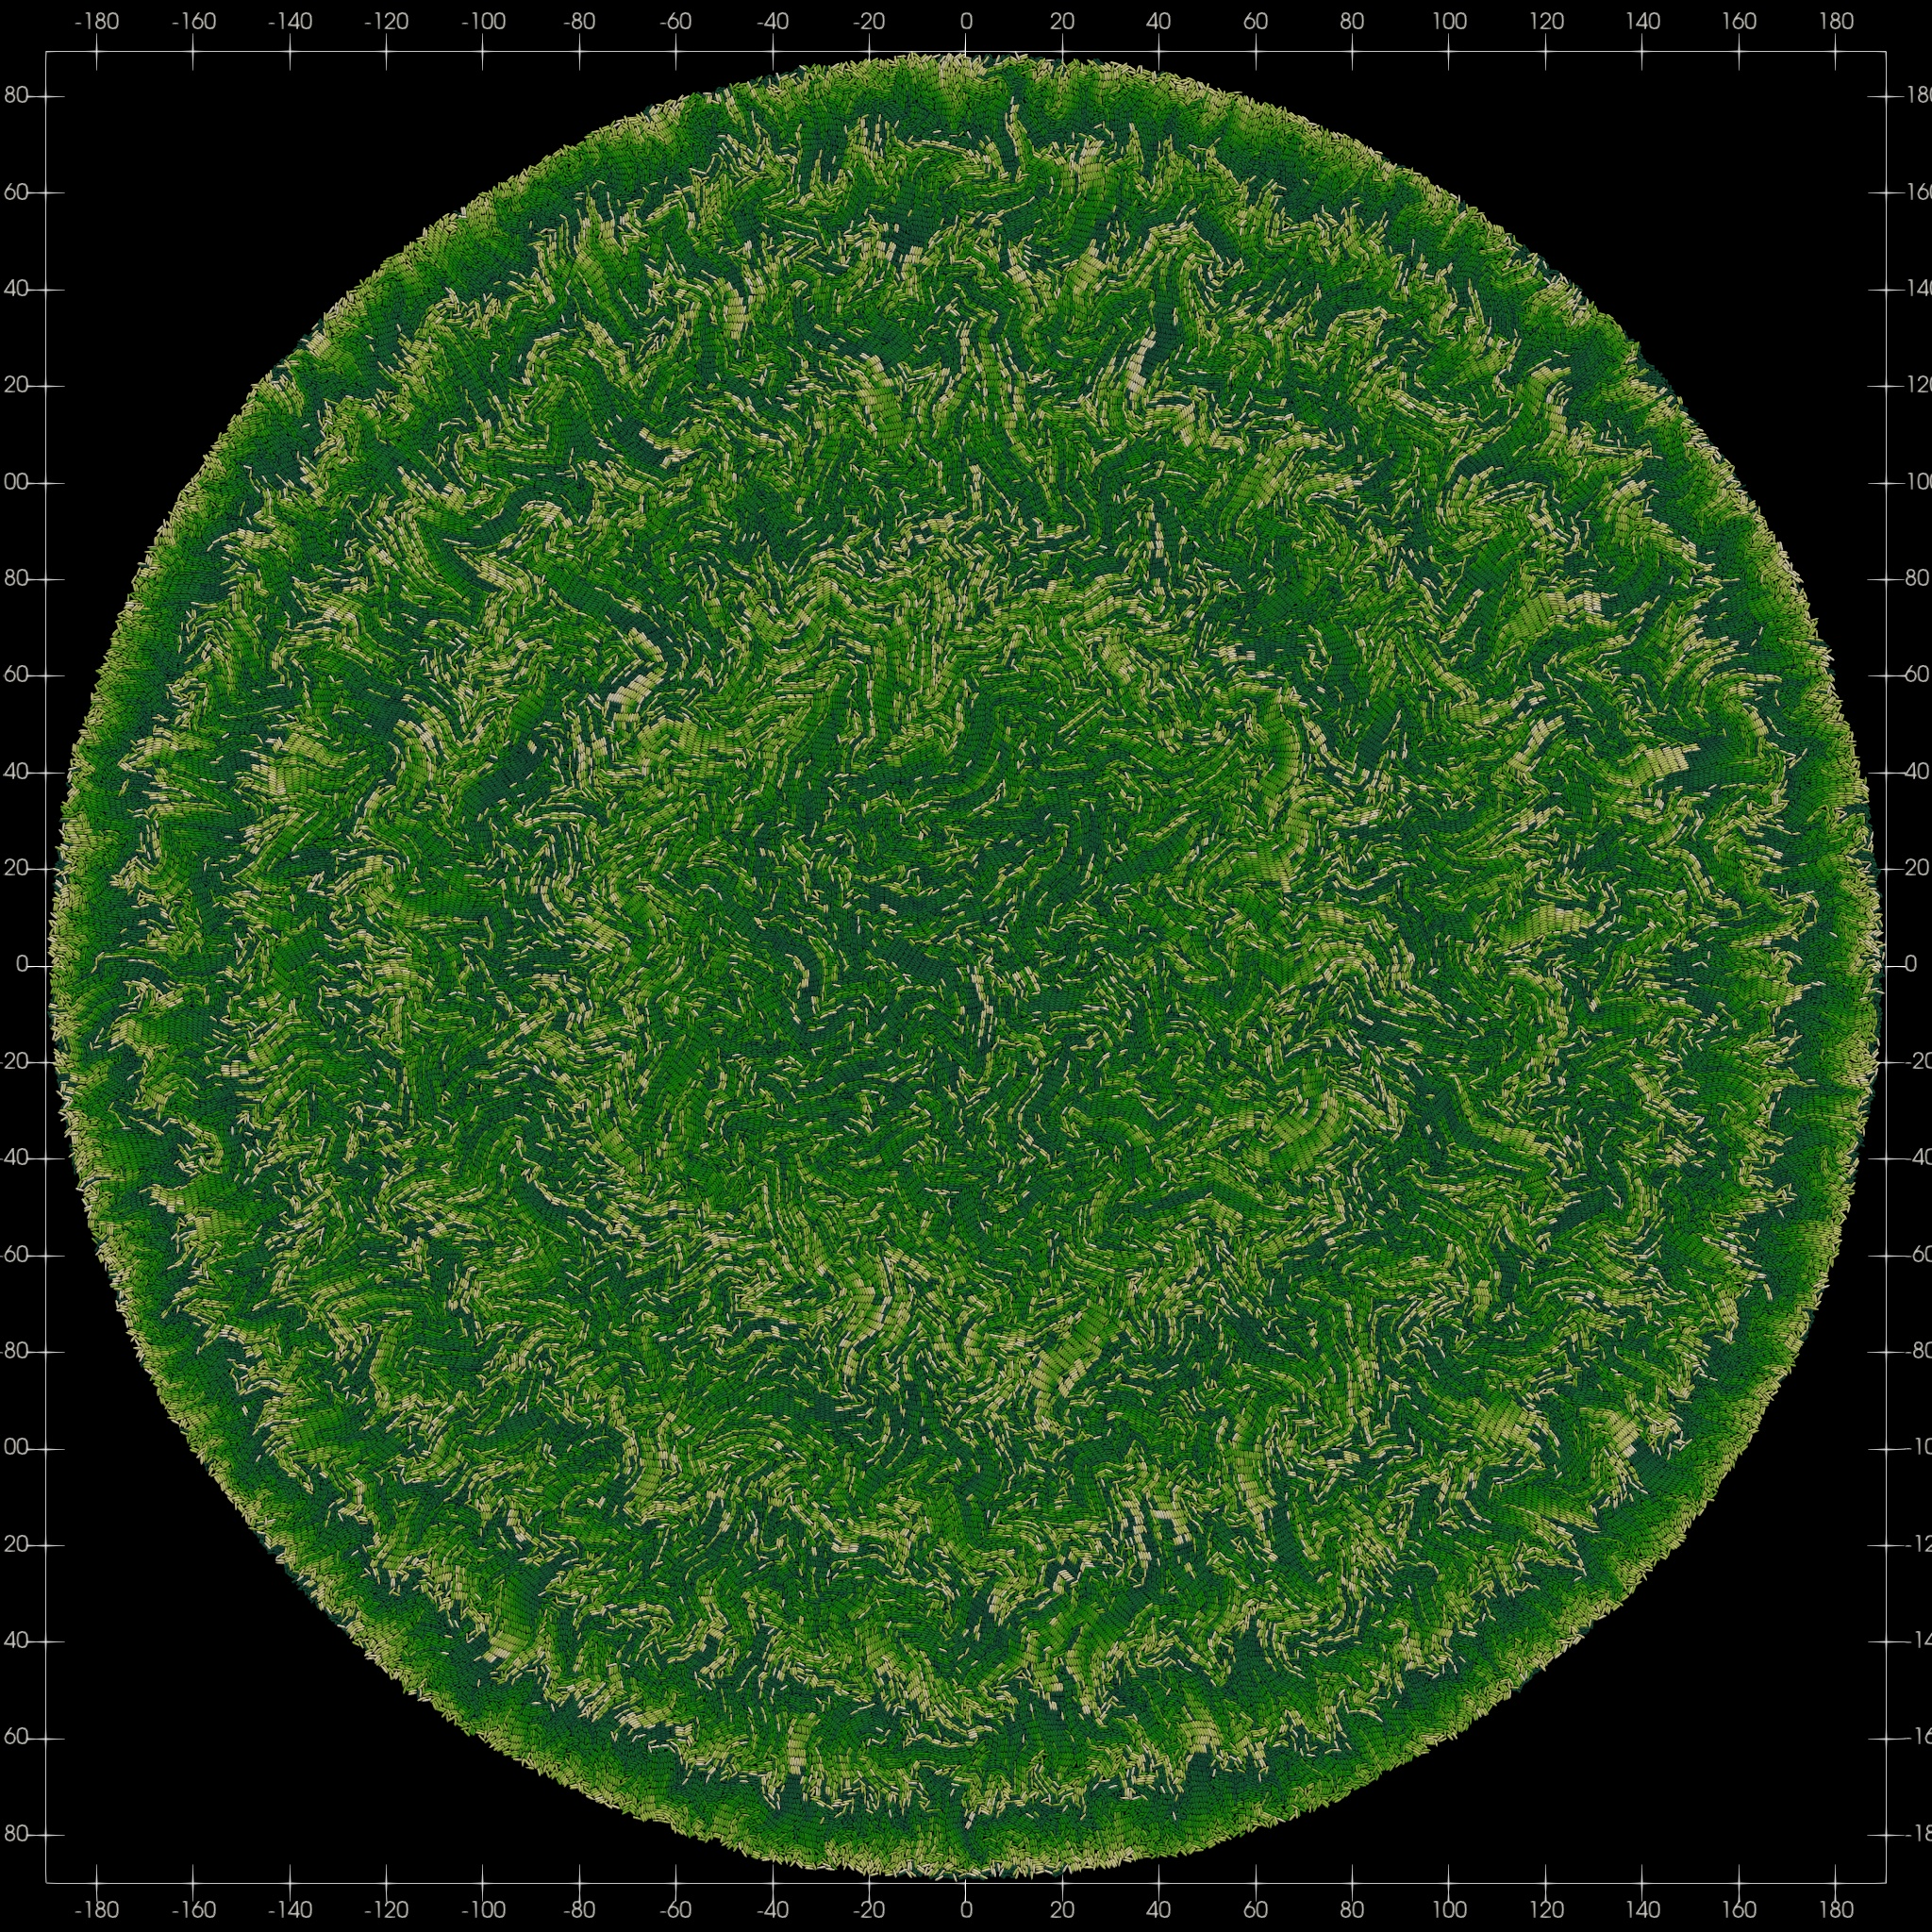
\includegraphics[width=\linewidth]{figures/growth/huge.jpeg}

    \caption{Snapshot of largest attainable colony size using the hard collision model with $\lambda=10^{-3}$ after 24h of wall time on 112 ranks on the CoolMUC-4 cluster. The colony has a radius of approximately $R \approx 195$ and consists of $168{,}339$ cells. The color indicates the length of the cells (short cells are darker, longer cells are lighter). Clear concentric ring patterns are visible, similar to those observed in smaller colonies (See \autoref{fig:pattern_formation}).}
    \label{fig:huge_colony_hard}
\end{figure}


\end{document}